%% ----------------------------------------------------------------------
%% START OF FILE
%% ----------------------------------------------------------------------
%%
%% Filename: thesis-bachelor.tex
%% Author: Fred Qi
%% Created: 2008-06-25 11:13:31(+0800)
%%
%% ----------------------------------------------------------------------
%%% CHANGE LOG
%% ----------------------------------------------------------------------
%% Last-Updated: 2016-02-09 14:49:44(-0700) [by Fred Qi]
%%     Update #: 123
%% ----------------------------------------------------------------------
%\documentclass{xduthesis}
\documentclass[bachelor,print,msfonts]{xduthesis}
\raggedbottom

% 免责声明:这是一份可用的毕业设计LaTeX模版,但是不保证格式完全正确,可能会有需要调整的地方
% 这里是可能用到的其他宏包,根据自己论文撰写的需要添加
\usepackage{listings}
\usepackage{overpic}
\lstset{language=TeX, basicstyle=\ttfamily}
\usepackage{booktabs}
\usepackage{multirow}
\usepackage{array}
\usepackage{graphicx}
%\usepackage{subfigure}
\usepackage{subfloat}

\newcommand{\figref}[1]{图\ref{#1}}
\newcommand{\sArt}{state-of-the-art}
\newcommand{\wyh}[1]{{\textcolor{blue}{#1}}}
\newcommand{\secref}[1]{Sec. \ref{#1}}
\newcommand{\tabref}[1]{Tab.~\ref{#1}}
\newcommand{\thudot}[1]{} % thubib.bst 定义每条参考文献最后的点\thudot
\graphicspath{{./}{./img/}{./fig/}{./image/}{./figure/}{./picture/}}
\newcommand{\bs}{\boldsymbol}
\usepackage{float}
\usepackage{longtable}
\def\allfiles{}

\begin{document}

%%%%%%%%%%%%%%%
%% 论文前置部分
%%%%%%%%%%%%%%%
\frontmatter

% 论文相关信息(封面)
\classid{1901015}
\studentid{19010100277}

\cschool{通信工程学院}
\ctitle{G-PCC Trisoup点云几何信息\\编码优化}
\cauthor{姚凯}
\cmajor{通信工程}
\csupervisor{张伟}

% 中英文摘要声明
%% ----------------------------------------------------------------------
%% START OF FILE
%% ----------------------------------------------------------------------
%% 
%% Filename: abstract.tex
%% Author: Fred Qi
%% Created: 2008-06-25 11:34:44(+0800)
%% 
%% ----------------------------------------------------------------------
%%% CHANGE LOG
%% ----------------------------------------------------------------------
%% Last-Updated: 2016-02-09 15:17:07(-0700) [by Fred Qi]
%%     Update #: 62
%% ----------------------------------------------------------------------

\begin{cabstract}
    随着新一代数字化媒体的出现,三维点云凭借其高精度、高自由度、高交互性等特征逐渐成为三维视觉媒体的重要代表。三维点云是一组三维的离散点集合,其中每个点都可以包含有空间几何坐标,颜色,反射率等信息,常被用来构建表征三维人物和场景的三维模型,并广泛应用于虚拟现实,增强现实,远程呈现和交互等应用中。但是随着点云点数和数据精度的不断提升,巨大的点云数据量给传输和存储都带来了前所未有的挑战。为了解决这一问题,国际运动图像专家组(Moving Picture Experts Group, MPEG)制订了用于点云压缩 G-PCC (Geometry Point Cloud compres)的标准。

    截止目前,MPEG G-PCC对点云的压缩是从几何信息和属性信息两方面分别进行。G-PCC提供了两种几何信息编码的方法,分别是八叉树几何编码和Trisoup几何编码。其中Trisoup编码为了使最后的熵编码更加的高效,编码得到的码流 更小,使用了动态 OBUF(Dynamic Optimal Binarization with Update On the fly)技术。动态OBUf中引入了上下文这一概念即编码当前待编码比特所能用到的一些条件信息的组合来辅助选取最佳的熵编码概率模型,这正是本文的主要研究内容。本文通过对现有动态OBUF所用到的上下文进行信息熵、条件熵的测量,依据熵值越小,上下文模型与当前待编码信息相关性越强的原理,优化了现有上下文的使用顺序。最后通过对比修改前后熵编码的性能,从而给出是否替换现有上下文模型的结论。

    将上下文按照条件熵递增的顺序使用后,在几何有损,属性有损(C2)条件下,相比现有的上下文模型,各类测试序列均呈现一定负增益,BD-GeomRate的平均取值为0.9\%,但是在某些序列呈现出较大的增益,如stanford\_area\_4\_vox20的D1取值为-3.8\%,D2取值为-3.6\%、landscape\_00014\_vox20的D1取值为-2.5\%,D2取值为-2.5\%。基于这些实验结果可以得出,单纯的对比各类上下文的熵值是无法选出最佳的上下文使用顺序的,有待进一步研究。同时针对某些序列拥有较大增益这一现象,本文认为引入自适应的上下文排序算法将带来一定性能增益。



\end{cabstract}

\begin{ckeywords}
    点云\quad 几何信息压缩\quad 动态OBUF\quad 熵编码\quad 上下文
\end{ckeywords}

\cthesistype{应用基础技术}


\begin{eabstract}
    With the emergence of a new generation of digital media, 3D point cloud has gradually become an important representative of 3D visual media due to its high precision, high degree of freedom, and high interactivity. 3D point cloud is a set of 3D discrete points, each of which can contain information such as spatial geometric coordinates, color, reflectivity, etc. It is often used to construct 3D models representing 3D characters and scenes, and is widely used in virtual Reality, augmented reality, telepresence and interactive applications. However, with the continuous improvement of point cloud points and data accuracy, the huge amount of point cloud data has brought unprecedented challenges to both transmission and storage. In order to solve this problem, the International Moving Picture Experts Group (MPEG) has developed a standard for point cloud compression G-PCC (Geometry Point Cloud compres).

    So far, MPEG G-PCC compresses point clouds from two aspects: geometric information and attribute information. G-PCC provides two geometric information encoding methods, namely Octree geometric encoding and Trisoup geometric encoding. Among them, Trisoup encoding uses dynamic OBUF (Dynamic Optimal Binarization with Update On the fly) technology in order to make the final entropy encoding more efficient and the encoded code stream smaller. Dynamic OBUf introduces the concept of context, that is, the combination of some conditional information that can be used to encode the current bit to be encoded to assist in selecting the best entropy encoding probability model, which is the main research content of this paper. This paper measures the information entropy and conditional entropy of the context used by the existing dynamic OBUF, and optimizes the use order of the existing context based on the principle that the smaller the entropy value, the stronger the correlation between the context model and the current information to be encoded. Finally, by comparing the performance of entropy coding before and after modification, the conclusion of whether to replace the existing context model is given.

    After the context is used in the order of increasing conditional entropy, under the condition of geometric loss and attribute loss (C2), compared with the existing context model, all kinds of test sequences show a certain negative gain, and the average value of BD-GeomRate It is 0.9\%, but it shows a large gain in some sequences. For example, the D1 value of stanford\_area\_4\_vox20 is -3.8\%, the value of D2 is -3.6\%, and the value of landscape\_00014\_vox20 The value of D1 is -2.5\%, and the value of D2 is -2.5\%. Based on these experimental results, it can be concluded that simply comparing the entropy values of various contexts cannot select the best context usage order, and further research is needed. At the same time, in view of the fact that some sequences have a large gain, this paper believes that the introduction of an adaptive context sorting algorithm will bring a certain performance gain.

\end{eabstract}

\begin{ekeywords}
    Point Cloud\quad Geometry Information Compression\quad dynamic OBUF\quad context
\end{ekeywords}

\ethesistype{Applied Basic Technology}

%% ----------------------------------------------------------------------
%%% END OF FILE 
%% ----------------------------------------------------------------------

% 生成论文的封面、声明页、中英文摘要
\makecover

% 论文目录
\tableofcontents

%%%%%%%%%%%%%%%
%% 论文正文
%%%%%%%%%%%%%%%
\mainmatter
\chapter{绪论}

\section{研究意义和背景}
近年来,三维点云模型已经成为继音频、图像、视频之后的新一代数字化媒体。点云是三维物体和场景的主要数据表示形式之一,用x、y 和 z 坐标描述几何形状,每个点都有额外的属性,如颜色、法线、透明度和材料属性。它们不需要像 Mesh 网格那样进行繁琐的三角计算,也不需要复杂的预处理\cite{ref1}。因其具有相对于传统二维平面媒体更高的视觉自由度和细节表达优势,点云在沉浸和交互式应用中具有优势。与此同时,其巨大的数据量也对当前多媒体生态系统的能力提出了挑战。为了降低点云数据的存储和传输对多媒体信号处理系统的压力,点云数据的压缩编码至关重要\cite{ref4}。

点云数据的获取主要是通过激光扫描技术,由一套成像传感器或一套摄像机来生成一个多维图像阵列并创建点云。随着 3D 采集技术的飞速发展,3D 传感器成本逐步降低并得到更多的推广应用,成熟的产品包括各种类型的 3D 扫描仪、LiDAR 和 RGB-D 相机。由这些传感器获取的三维数据可以提供丰富的几何信息(形状、大小、三维空间位置等)、特征信息(颜色、不透明率、反射率、反照率等)。为此,国际和国内多个标准化组织\cite{ref2}均已开始三维点云压缩编码标准的制订工作。2017 年 4 月,国际标准化组织 ISO 下设的 MPEG 运动图像专家组正式开始了三维点云压缩编码 PCC 标准制订,此后 MPEG 一直致力于不断改进点云压缩的性能。在 2020 年批准了两种用于点云压缩的编码标准:V-PCC(基于视频的点云压缩)和 G-PCC(基于几何的点云压缩)。其中,针对静态点云和动态获取点云的 G-PCC,它是直接对三维空间里的点云利用八叉树或者预测树按照几何信息进行编码,然后再用重建几何信息和原始点云进行重着色,在对重着色的点云进行属性编码。我国的数字音视频编解码技术标准工作组(AVS)于2019年12月成立了国内点云压缩专家工作组并开始封闭研发参考软件。经过多方面的努力,在2020年9月发布了第一版点云编码参考平台PCRMv1.0,截止到2023年1月3号,参考平台已更新到PCRMv9.0。

在对几何信息编码的研究中,得益于小米提出的一系列有关 Trisoup 的改进提案\cite{ref6,ref7,ref8,ref9,ref10,ref11},几何信息编码性能有了新的提升。 Trisoup 是基于八叉树编码的一种将对象表面表示为一系列三角形的编码方式,这样的处理大大降低了需要传输的点云几何信息,编码端仅需传输选取的用于构建表面三角形的顶点信息,利用这一信息重建出三角面片然后对三角面片进行射线追踪采样后便可重建出原始几何形状。另外,参考八叉树编码采用利用邻居信息来作为上下文,Trisoup 在编码顶点信息时也引入了上下文的概念\cite{ref13},这对改善其几何信息编码后进行熵编码时的编码环境,性能都有一定的提升,但由于上下文模型成熟度不高,仍然存在很多冗余条件或者错误的邻居信息。

%\begin{enumerate}
%    \item 博客链接,参考第三部分LaTeX入门:\href{https://levitate-qian.github.io/2020/12/01/latex-lecture/}{LaTeX模板分享} 
%    \item b站录播,视频后半部分:\href{https://www.bilibili.com/video/BV1Ef4y1v78w}{【西电MSC】2020第三次技术沙龙}
%\end{enumerate}

\section{研究内容}
现有点云压缩将从两方面进行,分别是几何信息压缩和属性信息压缩。其中几何信息的压缩是指利用某些编码方式来编码重建点云的几何坐标,并且在解码端可以恢复出具有三维位置信息的点。而属性信息的压缩针对重建点云中的点附带的一些属性信息,例如颜色、反射率等。目前 MPEG 批准的用于点云压缩的 G-PCC 编码标准\cite{ref17}中,首先进行几何编码,之后基于重建的几何信息再进行属性编码。本文重点研究几何信息编码。

目前 MPEG 针对 PCC 中的几何编码,采用的是基于八叉树的几何编码算法\cite{ref18}或者基于表面拟合的Trisoup几何编码算法\cite{ref19}。八叉树几何编码算法主要是通过将点云不断进行八叉划分,划分出 8 个节点,并用 8 个比特表示,根据子节点的占据情况,决定 8 个比特的 0,1 分布。接着对于占据的子节点进一步划分,直到划分到最小的节点为止,并最终通过熵编码对产生的码流进行压缩。Octree 几何编码常用于 TMC13,即动态获取点云。Trisoup几何编码算法常用于 TMC1,即静态获取且表面密集的点云。在 TMC1 几何信息编码中,常常先用八叉树划分到一定层次,然后应用 Trisoup 进行确定顶点和对顶点熵编码以达到压缩的目的,然后通过三角重建近似曲面进行解压缩,也就是说 Trisoup 是一种基于八叉树的几何编码方式。但是在当前几何信息编码标准测试环境中,对于每一个点云文件在进行编码时八叉树应该划分到哪一层都有固定的值,由参数 trisoupNodeSizeLog2 确定。

其中Trisoup算法为了使最后的熵编码更加的高效,编码得到的 bit 流更小,熵编码顶点信息过程中使用了动态 OBUF。顶点标识信息与顶点位置信息分开编码,用到了两组不同的上下文信息,同时上下文信息又分为主要信息与次要信息:主要信息用较少的 bit 数承载了绝大部分相关性信息,去除该相关性以后再进行熵编码,码流显然会减少;次要信息的动态使用则是动态 OBUF \cite{ref5}的特点所在,它会根据熵编码输出的值更新 LUT 以及上下文使用数量。因此,次要信息中的上下文顺序与熵编码码流的大小有着直接的关联,最佳的上下文顺序可以使熵编码码流达到最小值,有效提高熵编码效率。
本文主要分析研究Trisoup算法中的熵编码过程,在现有上下文基础上,通过测试次要信息中各个上下文的性能来决定其使用顺序。通过对比更改顺序前后在各个类型测试序列下的性能结果来评判上下文顺序是否得到优化。



\section{章节安排}
本论文一共分为五个章节,各个章节主要内容如下所述:

第一章:主要介绍了点云编码的研究背景和意义,同时也对本文的研究内容进行了阐述,另外还对本篇论文的整体结构进行了介绍。

第二章:介绍了G-PCC编解码整体流程,并对获取点云数据、几何信息编码、属性信息编码、动态OBUF以及编码性能的评价标准进行了详细的介绍。

第三章:首先介绍了Trisoup算法中编码顶点标识信息和顶点位置信息时用到的上下文信;其次开始介绍各个上下文信息的信息熵测量;然后,基于求得的信息熵,按照条件熵递增的顺序求得上下文排列顺序。求得局部最优的上下文顺序,用此来提高熵编码效率。

第四章:介绍了TMC13v20平台下的测试序列、测试条件以及对应条件下的测试结果与分析。

第五章:对全文进行了一个总结,分析了本次实验带来的增益与不足,对于不足之处,提出了后续可以进行改进的方向与思路。


%% ----------------------------------------------------------------------
%% START OF FILE
%% ----------------------------------------------------------------------
%% 
%% Filename: ch01-intro.tex
%% Author: Fred Qi
%% Created: 2011-03-14 18:22:25(+0800)
%% 
%% ----------------------------------------------------------------------
%%% CHANGE LOG
%% ----------------------------------------------------------------------
%% Last-Updated: 2014-11-24 16:57:28(+0300) [by Fred Qi]
%%     Update #: 43
%% ----------------------------------------------------------------------
\ifx\allfiles\undefined
\documentclass[bachelor,print,msfonts]{xduthesis}

% 这里是可能用到的其他宏包,根据自己论文撰写的需要添加
\usepackage{listings}
\usepackage{overpic}
\lstset{language=TeX, basicstyle=\ttfamily}

\newcommand{\figref}[1]{图\ref{#1}}
\newcommand{\sArt}{state-of-the-art}
\newcommand{\wyh}[1]{{\textcolor{blue}{#1}}}
\newcommand{\secref}[1]{Sec. \ref{#1}}
\newcommand{\tabref}[1]{Tab.~\ref{#1}}
\newcommand{\thudot}[1]{} % thubib.bst 定义每条参考文献最后的点\thudot
\graphicspath{{./}{./img/}{./fig/}{./image/}{./figure/}{./picture/}}
\newcommand{\bs}{\boldsymbol}
\usepackage{float}
\begin{document}

\mainmatter
\fi
\chapter{点云压缩}
%\label{cha:intro}
\section{概述}
点云是空间中一组用来表示三维物体、场景的空间结构和表面属性信息的无规则分布的离散点集。其中的每个点都包含几何位置的三维信息,同时也根据应用场景的不同,还会包括不同的属性信息,比如颜色、反射率等。点云的应用十分广泛,如虚拟现实\cite{ref15}、无人驾驶、辅助医疗\cite{ref14}、文物数字化保护等领域。

近年来,随着 3D 扫描技术的迅速发展、采集设备的精度不断提高、图像传感器的改善,使得拥有数以百万计个点的点云模型得以实现,从而为用户带来更加逼真的视觉体验,但与此同时也对数据的存储和传输带来了巨大的压力。在现有的点云压缩编码方法中,国内由AVS提出的PCEM平台以及国外由MPEG提出的G-PCC标准中都是将点云几何信息和属性信息分开进行编码,并且属性信息的编码是建立在重建后的几何信息之上。因此,如何有效地对点云的几何与属性信息进行压缩,是目前科研工作的重点,也是目前研究的热点问题\cite{ref4}。

本章的内容安排如下:2.2介绍了点云的获取方法,2.3介绍了目前MPEG的G-PCC框架\cite{ref12},2.4介绍了几何信息编码方法,2.5介绍了属性信编码方法,2.6介绍了点云压缩性能评价标准。

\section{点云的获取}
%\label{sec:motivation}
截止目前,主流的点云获取方法有计算机生成、3D激光扫描、3D摄影测量这三种。获取方法的不同,得到的点云数据也不同:计算机生成的点云一般是表示虚拟物体或者场景,被称为静态点云;3D 激光扫描仪可以快速获取被扫描物体或场景的表面坐标、属性数据,为三维物体或场景建立静态点云模型,同时它也能生成动态获取点云,比如安装在无人驾驶汽车上的LiDAR 扫描仪就是一种先进的3D 激光扫描仪,它每秒获得的点云可达百万级;3D摄影测量获取的点云则是动态的点云模型,这样的点云能像视频一样播放,因此在医学影像领域备受青睐。

\begin{figure}[htbp]
    %是可选项 h表示的是here在这里插入,t表示的是在页面的顶部插入
    \centering
    \subfloat[静态点云]{
        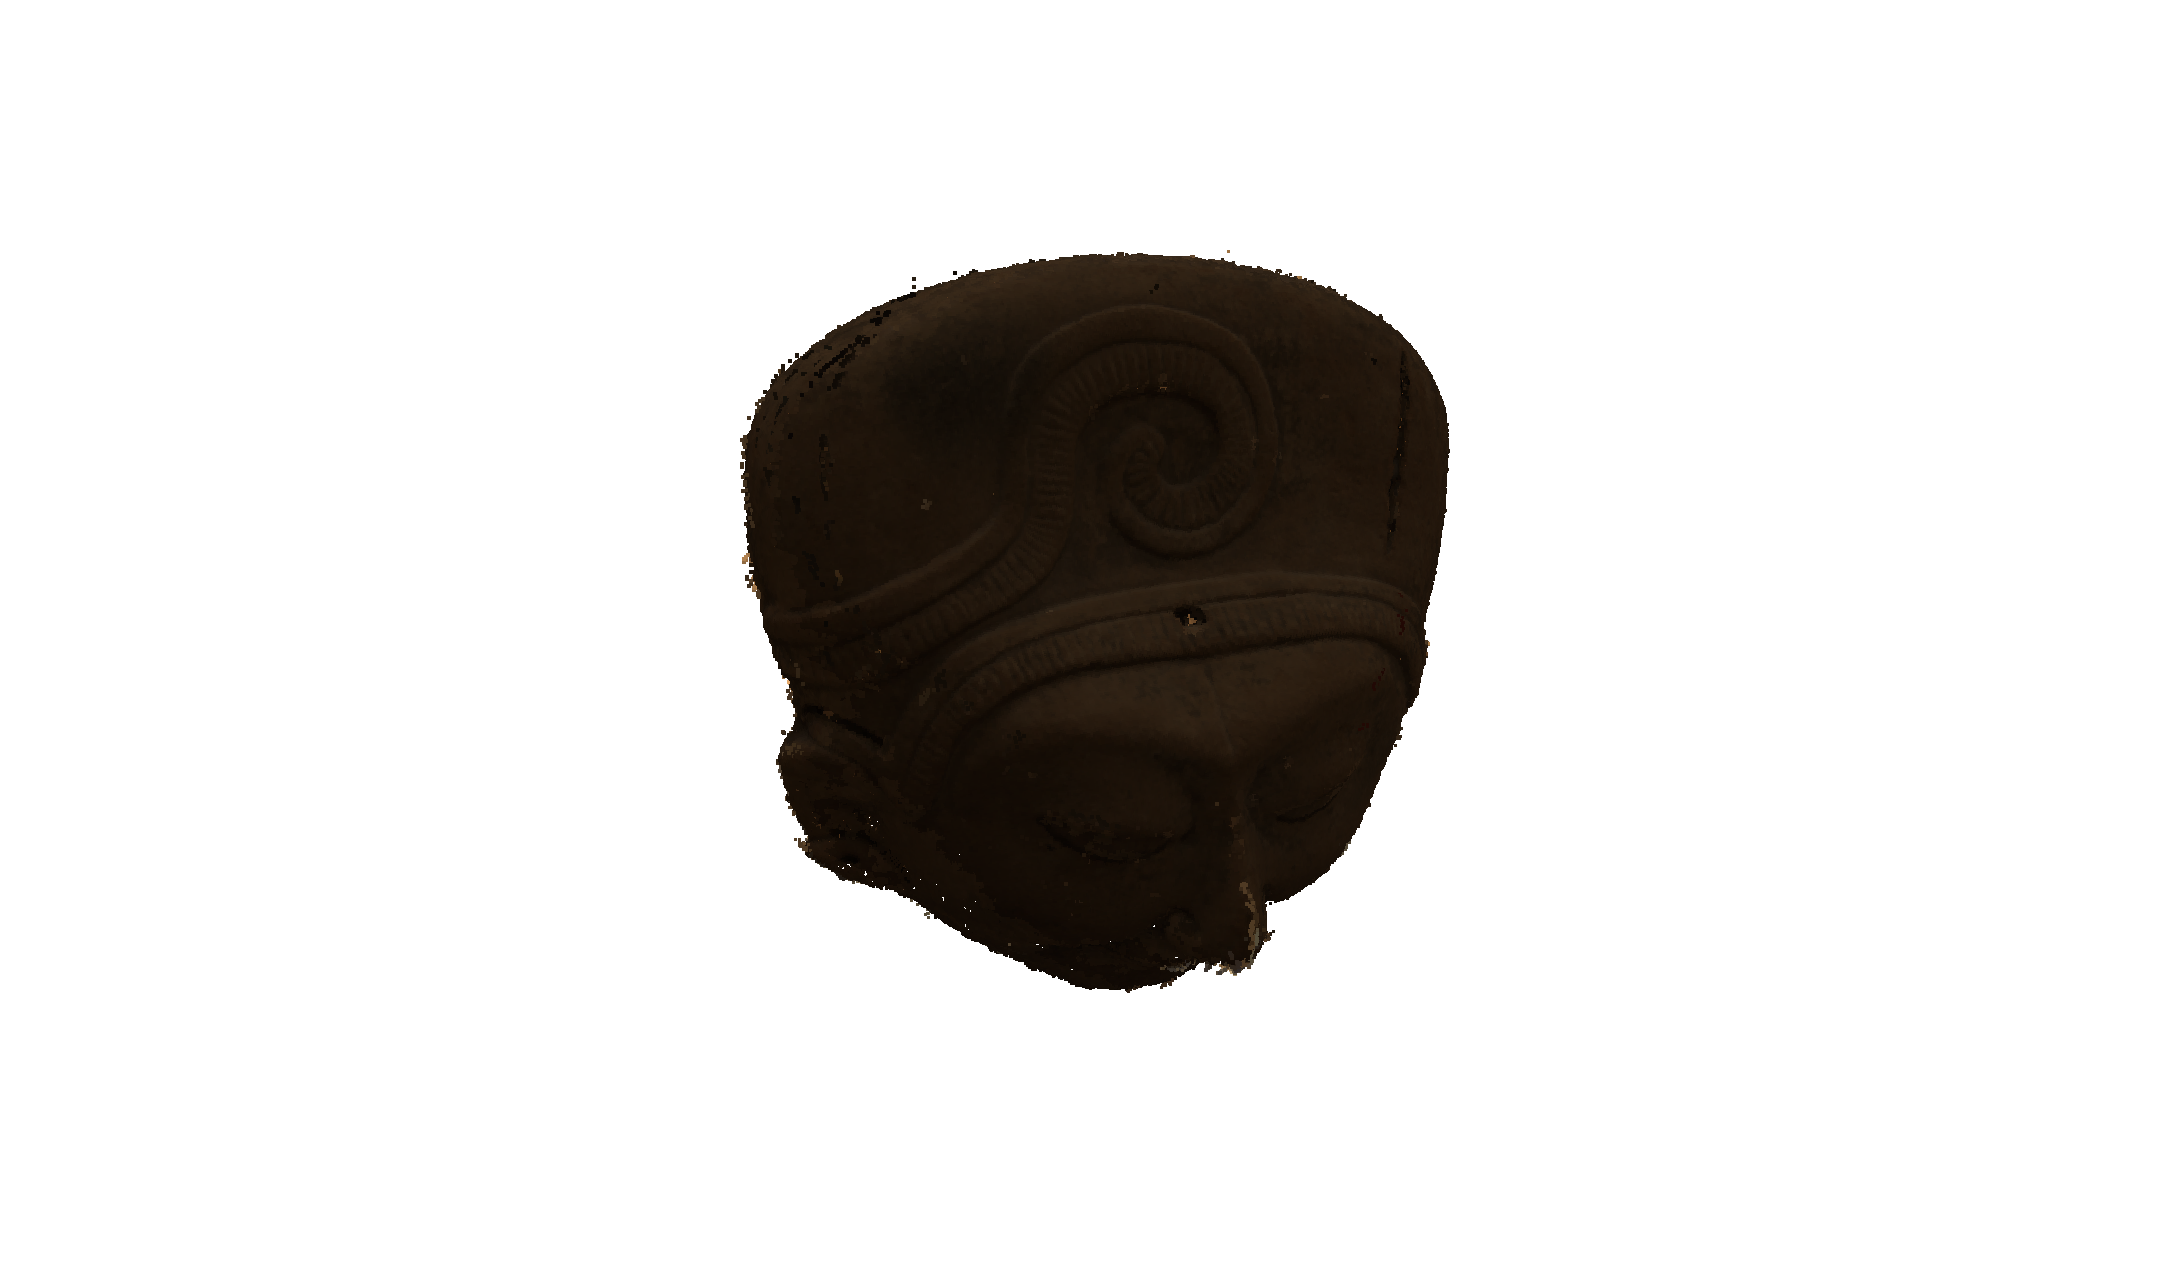
\includegraphics[scale=0.1]{image/静态点云示意图.png}
    }
    \hspace{0.1in}
    \subfloat[动态点云]{
        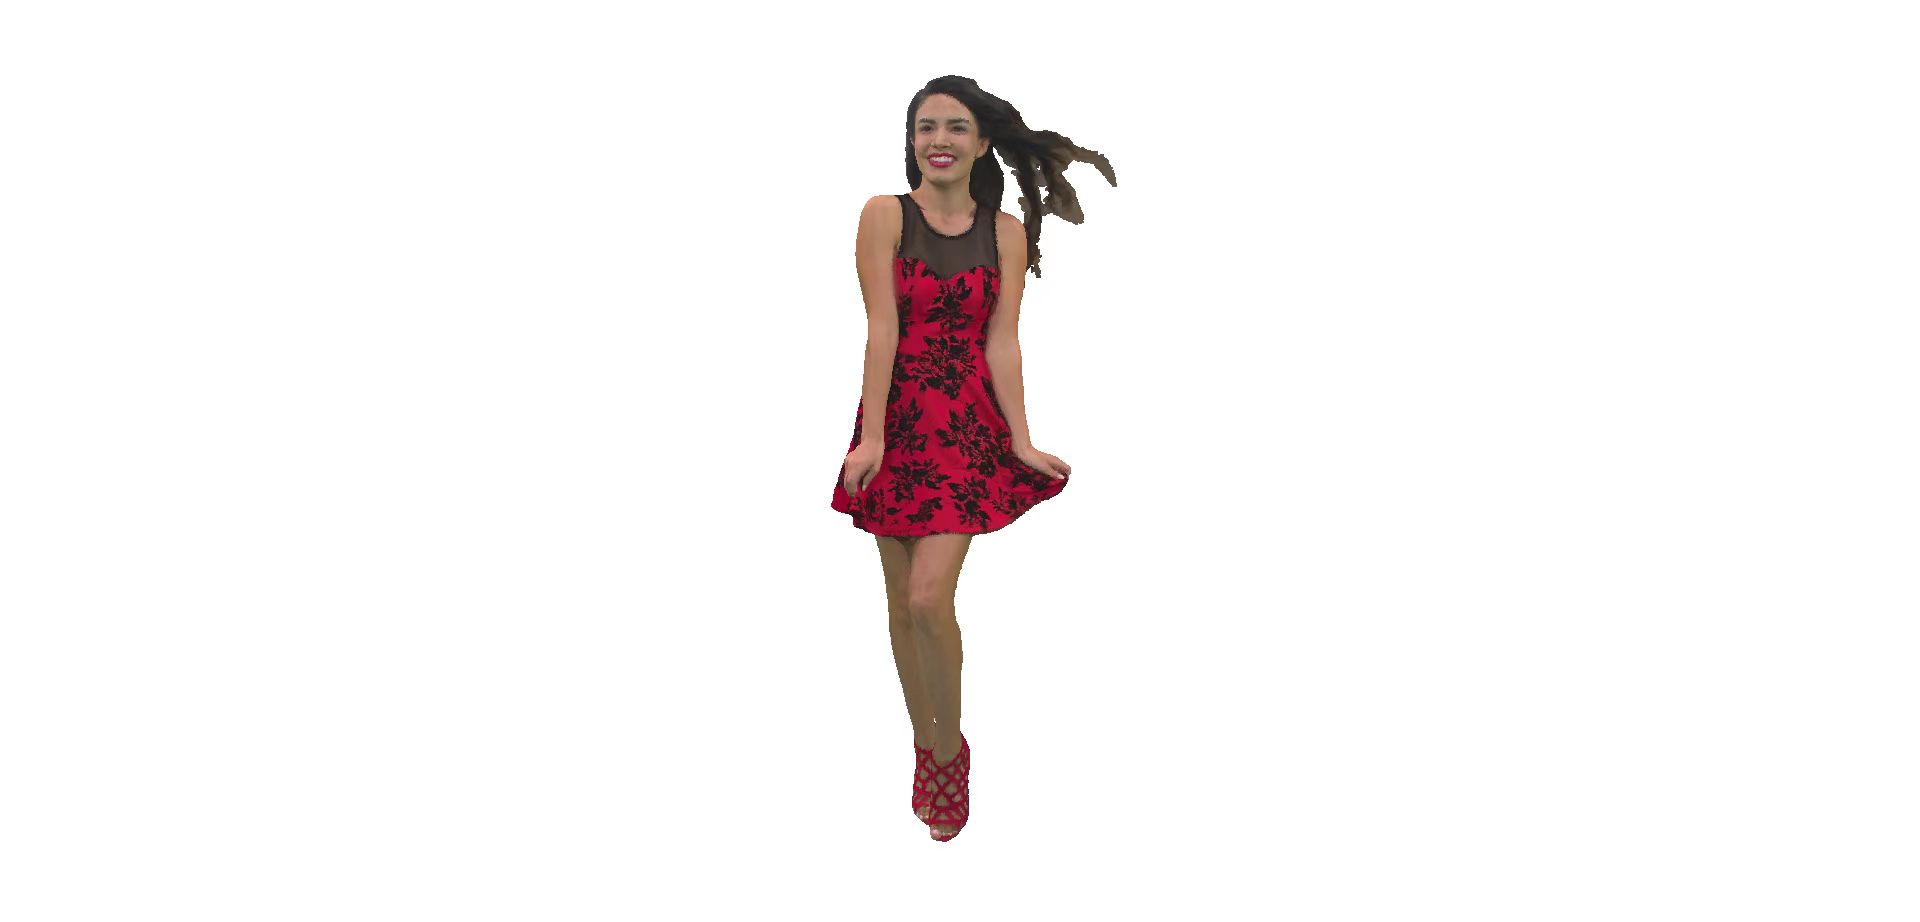
\includegraphics[scale=0.1]{image/动态点云示意图.jpg}
    }
    \hspace{0.1in}
    \subfloat[动态获取点云]{
        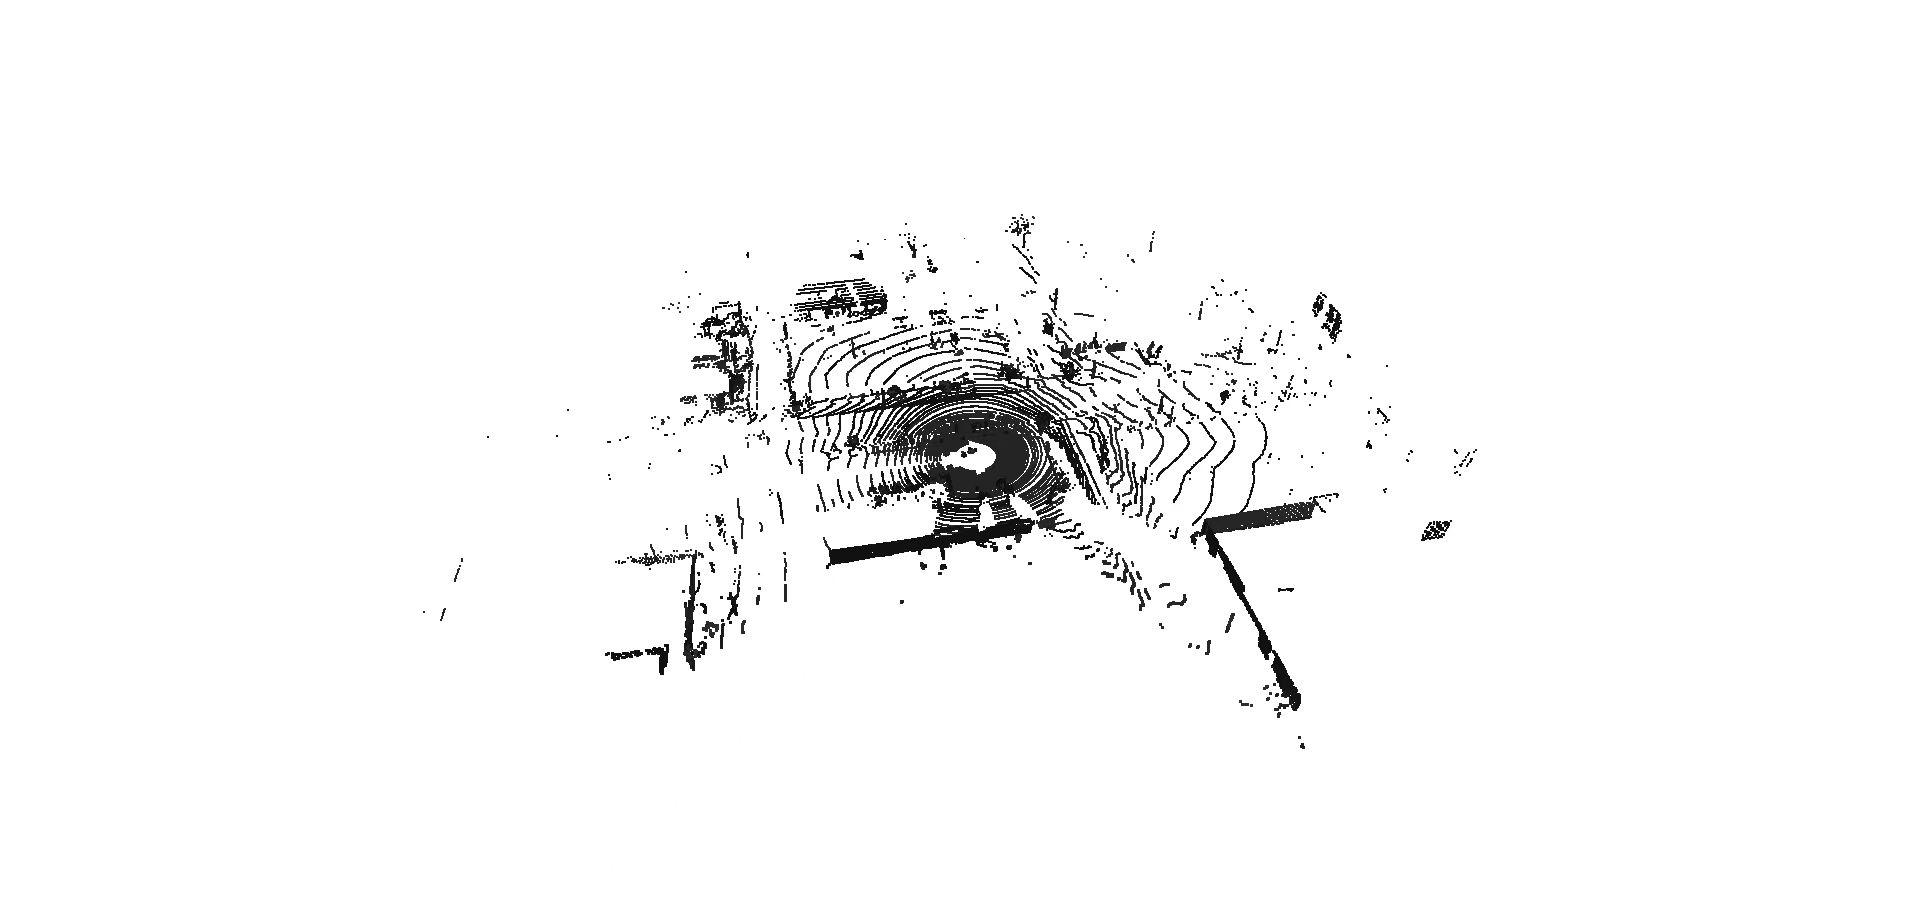
\includegraphics[scale=0.1]{image/动态获取点云.jpg}
    }
    \caption{三类点云示意图}
    \label{fig:三类点云示意图}
\end{figure}

点云获取技术的不断更新与发展,使得获得的点云模型精度不断提高,数量也急剧增大。越来越大的行业需求压力,促使着点云压缩技术的发展与标准化工作的展开。其中,MPEG提出的G-PCC标准主要针对静态点云和动态获取点云进行压缩,而V-PCC主要针对静态获取的动态点云进行压缩。

\section{GPCC框架}
本文主要对国际动态图像专家组MPEG提出的几何点云压缩(G-PCC)展开研究,该组织在为了方便测试和研究,推出了TMC13(Test Model for Category1 and Catgory3) 模型软件\cite{ref16},作为公开探索实验的参考平台。这一平台的具体编解码框架如图\ref{fig:编解码流程图}所示。从图中可以看出,不论是在编码端还是在解码端,几何信息和属性信息的编码都是分开进行的,以编码端为例:

几何信息编码首先对原始点云数据进行预处理,将点云几何信息进行坐标转换,使得变换后的点都在包围(BoundingBox)内再进行量化和重复点去除工作。然后对包围盒进行八叉树(Octree)划分,通过递归细分立方体的方法来构建八叉树结构。立方体每次八等分被划分成八个子立方体,之后再对非空的子立方体进行八等分,直到划分到体素大小为 1×1×1,使用占用码(occupancy code)表示一个立方体是否包含子立方体,1表示被占据,0表示不被占据,最后将占位信息送入熵编码器得到几何码流。Octree几何编码常用于TMC13,即动态获取点云,而针对表面稠密的静态点云(TMC1),Trisoup几何编码方式更具优势。Trisoup 是一种基于八叉树的几何编码方式,该方法先用八叉树划分到一定体素大小,然后应用 Trisoup 进行确定顶点和对顶点熵编码以达到压缩的目的,然后通过三角重建近似曲面进行解压缩,后续的属性编码也是基于重建后的点云进行。
\begin{figure}[htbp]
    %是可选项 h表示的是here在这里插入,t表示的是在页面的顶部插入
    \centering
    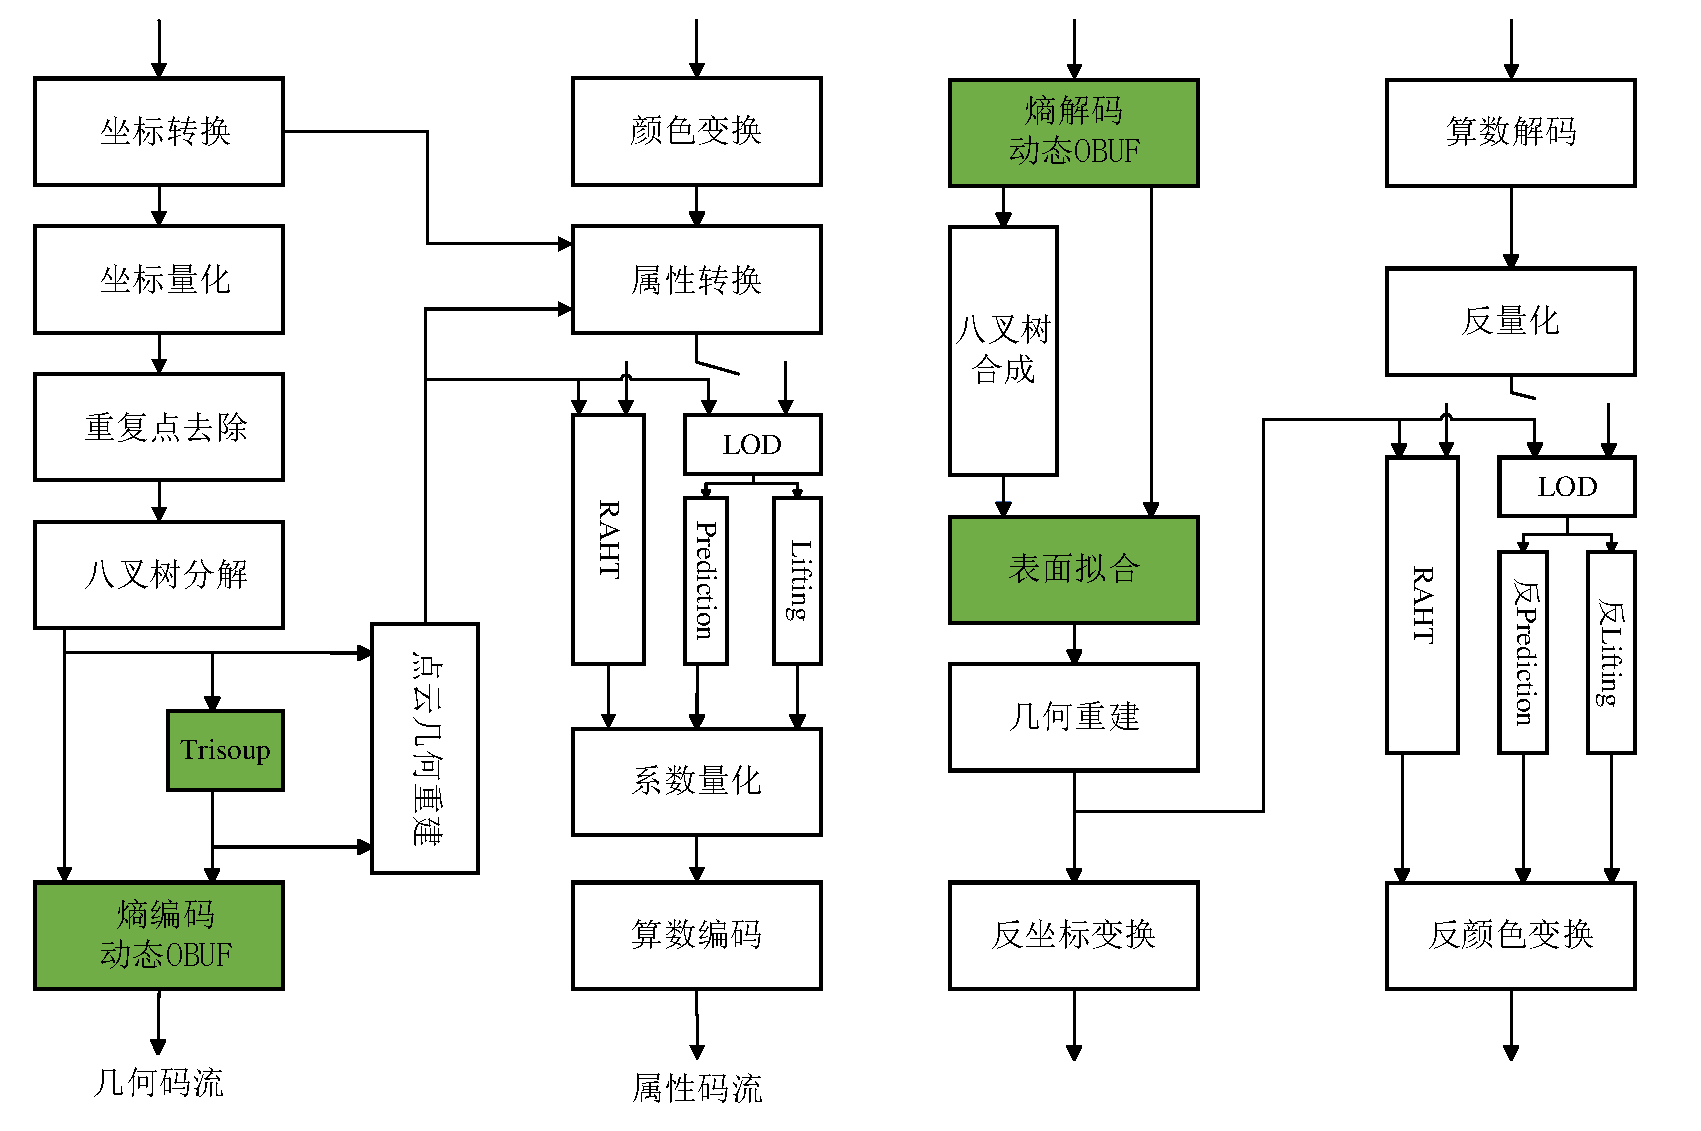
\includegraphics[scale=0.5]{image/编解码流程图ykv2.pdf}
    \caption{编解码流程图}
    \label{fig:编解码流程图}
\end{figure}

属性信息编码首先选择是否对对输入的属性信息进行颜色空间转换,目前TMC13 平台支持将颜色属性从 GBR 转换成 YUV 空间。当几何有损时,需要对点云进行属性转换,也就是对几何重建出来的点云重新赋予颜色信息。之后进行属性信息编码,根据不同的测试序列和条件选择适合的编码方式。接着将属性残差经过系数量化处理,最后通过熵编码得到最终的属性码流。

解码端对码流的处理流程即为编码端的逆过程。

另外,在现有的G-PCC标准中,使用Trisoup几何编码方式时,其熵编码过程用到了动态更新的最佳二值化技术(动态OBUF),相比于OBUf,该技术将上下文信息分为了主要信息和次要信息两部分,其中,主要信息用较少的bir位包含了上下文信息中最相关的部分,因此它不会变化;相反,次要信息会根据已使用的上下文信息能否将点云有效的区分开来进而来决定是否继续使用下一bit位上下文信息。这也是本文的主要研究内容。
\section{几何信息编码}
点云数据中一般存储着几何坐标、颜色、法线等信息。其中几何信息是必不可少的,它在物体的三维重建过程中起着决定性的作用。点云的几何形状通常用特定于应用程序的空间表示,其中点的位置可以用浮点数表示。因此,需要一个预处理步骤,将应用程序特定的空间转换为有限分辨率的内部空间。几何信息预处理的步骤一般包括:坐标转换,坐标量化、重复点去除。其具体过程如下:
\subsection{坐标转换}
获取到的原始点云中,各个点的位置通常是无规则的,并且通常由浮点数表示。因此,为了方便后续对几何信息进行压缩,首先将原始坐标系中点的位置坐标${\rm{X}}_{\rm{n}}^{orig}$用公式\ref{fig:公式1}转换为内部坐标系下的坐标${\rm{X}}_{\rm{n}}^{{\mathop{\rm int}}}$。
\begin{equation}
    {X_n} = ({\rm{X}}_n^{orig} - T)/s
    \label{fig:公式1}
\end{equation}

其中,$T=({t_x},{t_y},{t_z})$。参数$T$和$s$由包围盒$[0,{2^d})^3$中的点位置坐标${\rm{X}}_{\rm{n}}^{{\mathop{\rm int}}}$,$n = 1,...,N$(其中$ D $是非负整数参数)决定。

当采用八叉树几何编码时,$1/s$由$positionQuantizationScale$参数决定,$T = (\min x_n^{orig},\min y_n^{orig},\min z_n^{orig})$,d由公式\ref{fig:公式2}确定:
\begin{equation}
    d = Ceil(Lo{g_2}(Max(x_n^{{\mathop{\rm int}} },y_n^{{\mathop{\rm int}} },z_n^{{\mathop{\rm int}} },n = 1, \ldots ,{N_{orig}}) + 1))
    \label{fig:公式2}
\end{equation}
$[0,{2^d})^3$是最小的包围盒,所有的内部点位置坐标都在这个边长${2^d}$的立方体内。

当采用Trisoup几何编码时,s由参数$trisoupQuantizationBits$确定,T=[0,0,0],d由$trisoupNodeSizeLog2$参数确定。

\subsection{坐标量化}
在压缩之前,点位置坐标在内部被表示为$d$位非负整数。为了获得这些整数,点的位置坐标在内部坐标系中被量化取整。设${\rm{X}}_{\rm{n}}^{{\mathop{\rm int}}}$表示内部坐标系中的点位置坐标,量化公式如公式\ref{fig:公式3}所示:
\begin{equation}
    \left\{\begin{array}{l}
        x^{k}={round}\left(\frac{{x}^{\prime}}{Q S}\right) \\
        y^{k}={round}\left(\frac{y^{\prime}}{Q S}\right)   \\
        z^{k}={round}\left(\frac{{z}^{\prime}}{Q S}\right)
    \end{array}\right.
    \label{fig:公式3}
\end{equation}

其中,$QS$为量化步长,这里$round(s)$函数的功能是返回距$s$最近的整数,定义如下:
\begin{equation}
    {round}(s)=\left\{\begin{array}{cc}
        {int}(s+0.5)   & { if } s \geq 0 \\
        -{int}(-s+0.5) & { if } s<0
    \end{array}\right.
\end{equation}

\subsection{重复点去除}
量化之后会产生大量位置坐标相同的点,称为重复点。可以将具有相同量化坐标的重复点进行删除操作。坐标量化和删除重复点的过程称为体素化,也就是将一个体素内的所有点都量化到体素中心。如果一个体素内包含任意点云中的点,则称该体素被占用。

\subsection{八叉树编码}
八叉树是一种自顶向下的广度优先的树状数据结构,它可以用来存储表示三维空间物体和场景的几何信息。八叉树中的每个节点都代表着一个对应的正方体。对于每个非空的节点,可以将其继续划分为八个子节点,直至划分到叶子节点,即指定精度下的三维空间的最小单元。在对点云几何信息进行预处理之后,将对点云几何信息进行几何编码,首先将点云中各点的坐标转换为二进制表示。如果各点的几何位置用三维笛卡尔坐标表示为$(X,Y,Z)$,$n=0, …, N-1$,其中$N$是点云的总点数,那需要将其$X、Y、Z$坐标数值转化为$K$位比特表示的二进制数值:
\begin{equation}
    \left\{\begin{array}{l}
        X^{n}=\left(x_{K-1}^{n} x_{K-2}^{n} \cdots x_{1}^{n} x_{0}^{n}\right) \\
        Y^{n}=\left(y_{K-1}^{n} y_{K-2}^{n} \cdots y_{1}^{n} y_{0}^{n}\right) \\
        Z^{n}=\left(z_{K-1}^{n} z_{K-2}^{n} \cdots z_{1}^{n} z_{0}^{n}\right)
    \end{array}\right.
\end{equation}

按照莫顿码的生成规则,可以将点云中第$n$个点的三维几何坐标的三个维度上的$K$位比特表示的二进制数值逐位交叉排列,形成一个新的$3K$位比特表示的二进制数,也就是对应的莫顿码,表示如下:
\begin{equation}
    M^{n}=\left(x_{K-1}^{n} y_{K-1}^{n} z_{K-1}^{n}, x_{K-2}^{n} y_{K-2}^{n} z_{K-2}^{n}, \ldots x_{1}^{n} y_{1}^{n} z_{1}^{n}, x_{0}^{n} y_{0}^{n} z_{0}^{n}\right)
\end{equation}

将每三个比特用八进制数表示$
    m_{n}^{k}=\left(x_{n}^{k} x_{n}^{k} x_{n}^{k}\right), n=0,1, \ldots, N-1
$ , 则$K$点对应的莫顿码可以表示成:
\begin{equation}
    M^{n}=\left(m_{K-1}^{n} m_{K-2}^{n} \ldots m_{1}^{n} m_{0}^{n}\right)
\end{equation}

可以看出,每个点的坐标用莫顿码表示之后形成了$K$个八进制数排列组成的数据。由于八进制数的所有的取值情况可以表示8种情况,正好可以与八个子节点一一对应,而且随着$k$值的减小,每个八进制数都代表一层更深的八叉树划分。这样在每一层划分八叉树节点时,就可以很好的判断当前待划分的点要被划分至哪个子节点中。
\subsection{Trisoup几何编码}
Trisoup几何编码方式常用于TMC1,即静态获取且表面密集的点云。在几何信息编码中,常常先用八叉树划分到一定层次,然后应用Trisoup进行确定顶点和对顶点熵编码以达到压缩的目的,然后通过三角重建近似曲面进行解压缩,也就是说Trisoup是一种基于八叉树的几何编码方式。但是在当前几何信息编码标准测试环境中,对于每一个点云文件在进行编码时八叉树应该划分到哪一层都有固定的值,由参数$trisoupNodeSizeLog2$确定。

Trisoup几何编码主要分四个步骤进行:
\begin{figure}[h]
    %是可选项 h表示的是here在这里插入,t表示的是在页面的顶部插入
    \centering
    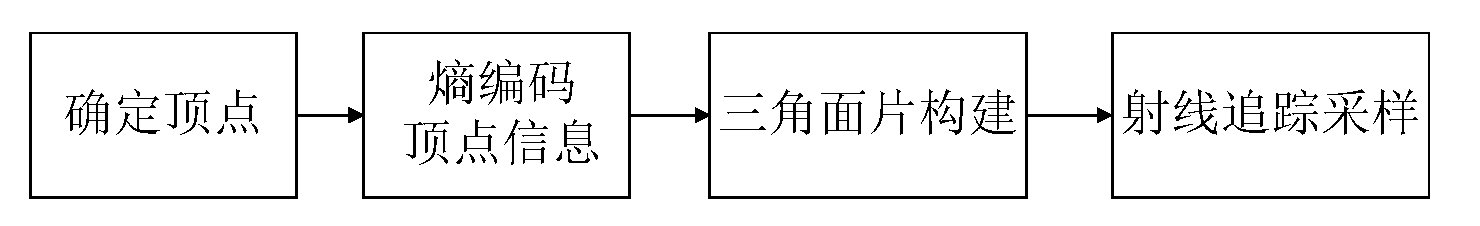
\includegraphics[scale=0.5]{image/Trisoup流程图_crop.pdf}
    \caption{Trisoup流程图}
\end{figure}

1、确定顶点。几何图形在每个块中表示为一个至多与块的每条边相交一次的曲面。由于一个块有12条边,所以在一个块中最多可以有12个这样的交点。每一个这样的交点称为顶点。当且仅当共享该边的所有块中与该边相邻的块中至少有一个已占用的体素时,才能检测到沿该边的顶点。检测到的顶点沿边的位置是共享该边的所有块中,所有与该边相邻的体素沿边的顶点的平均位置。

2、熵编码顶点信息。顶点信息包含两部分:一个是标识信息,即标识所有被占据的叶子节点中哪些边上有顶点,也称为边被占据,被占据标识为 1,不被占据标识为 0;另一个是顶点位置信息,对于每个被占据的边,顶点位置信息被量化为 2bit。最后利用算数编码器对标识信息与顶点位置信息进行熵编码。

3、三角面片构建。根据三角形投影面积大小确定主导轴、求出质心坐标以及质心偏移量、根据方位角信息对顶点进行排序。最后将顶点与质心组合,构建三角面片。如图\ref{fig:三角面片构建}所示。
\begin{figure}[h]
    %是可选项 h表示的是here在这里插入,t表示的是在页面的顶部插入
    \centering
    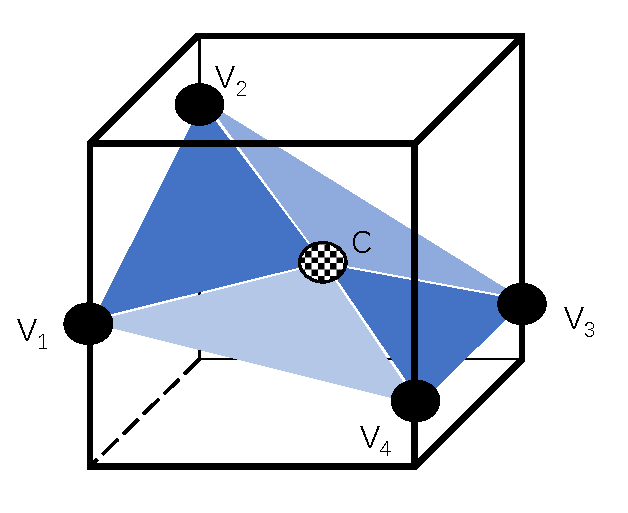
\includegraphics[scale=0.5]{image/三角面片构建v2.pdf}
    \caption{三角面片构建示意图}
    \label{fig:三角面片构建}
\end{figure}

4、射线追踪采样。以三角面片在主轴方向上的投影面为射线起点,射线追踪的间隔由高层语法元素决定,同时会根据重建后的点云数量改变间隔大小。射线追踪采样的核心是利用Muller-Trumbore算法\cite{ref22},判定射线是否与三角面片有交点,产生的交点便是重建点云。如图\ref{fig:射线追踪采样}所示。
\begin{figure}[htbp]
    %是可选项 h表示的是here在这里插入,t表示的是在页面的顶部插入
    \centering
    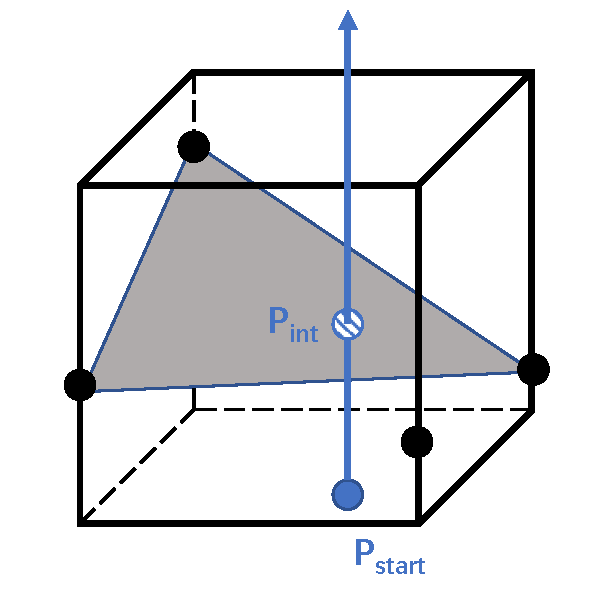
\includegraphics[scale=0.5]{image/射线追踪v2.pdf}
    \caption{射线追踪采样示意图}
    \label{fig:射线追踪采样}
\end{figure}

为了使熵编码更加的高效,编码得到的bit流更小,熵编码顶点信息过程中使用了动态OBUF。顶点标识信息与顶点位置信息分开编码,用到了两组不同的上下文信息,同时上下文信息又分为主要信息与次要信息:主要信息用较少的bit数承载了绝大部分相关性信息,去除该相关性以后再进行熵编码,码流显然会减少;次要信息的动态使用则是动态OBUF的特点所在,它会根据熵编码输出的值更新LUT以及上下文使用数量。
\subsection{动态OBUF}
\label{动态OBUF}
在MPEG给出的TMC13v20参考代码中,采用Trisoup几何编码方式时,最后将顶点的标识信息、顶点的位置信息进行熵编码时,采用的是基于动态更新的最佳二值化的熵编码器(动态OBUF),其编码框架如图\ref{fig:动态OBUF流程图}所示,动态OBUF的基本工作流程与OBUF一致,它只是新加入了上下文的动态缩减过程,以达到使编码当前符号的概率模型更加迅速的趋于信源概率模型的目的。
\begin{figure}[h]
    %是可选项 h表示的是here在这里插入,t表示的是在页面的顶部插入
    \centering
    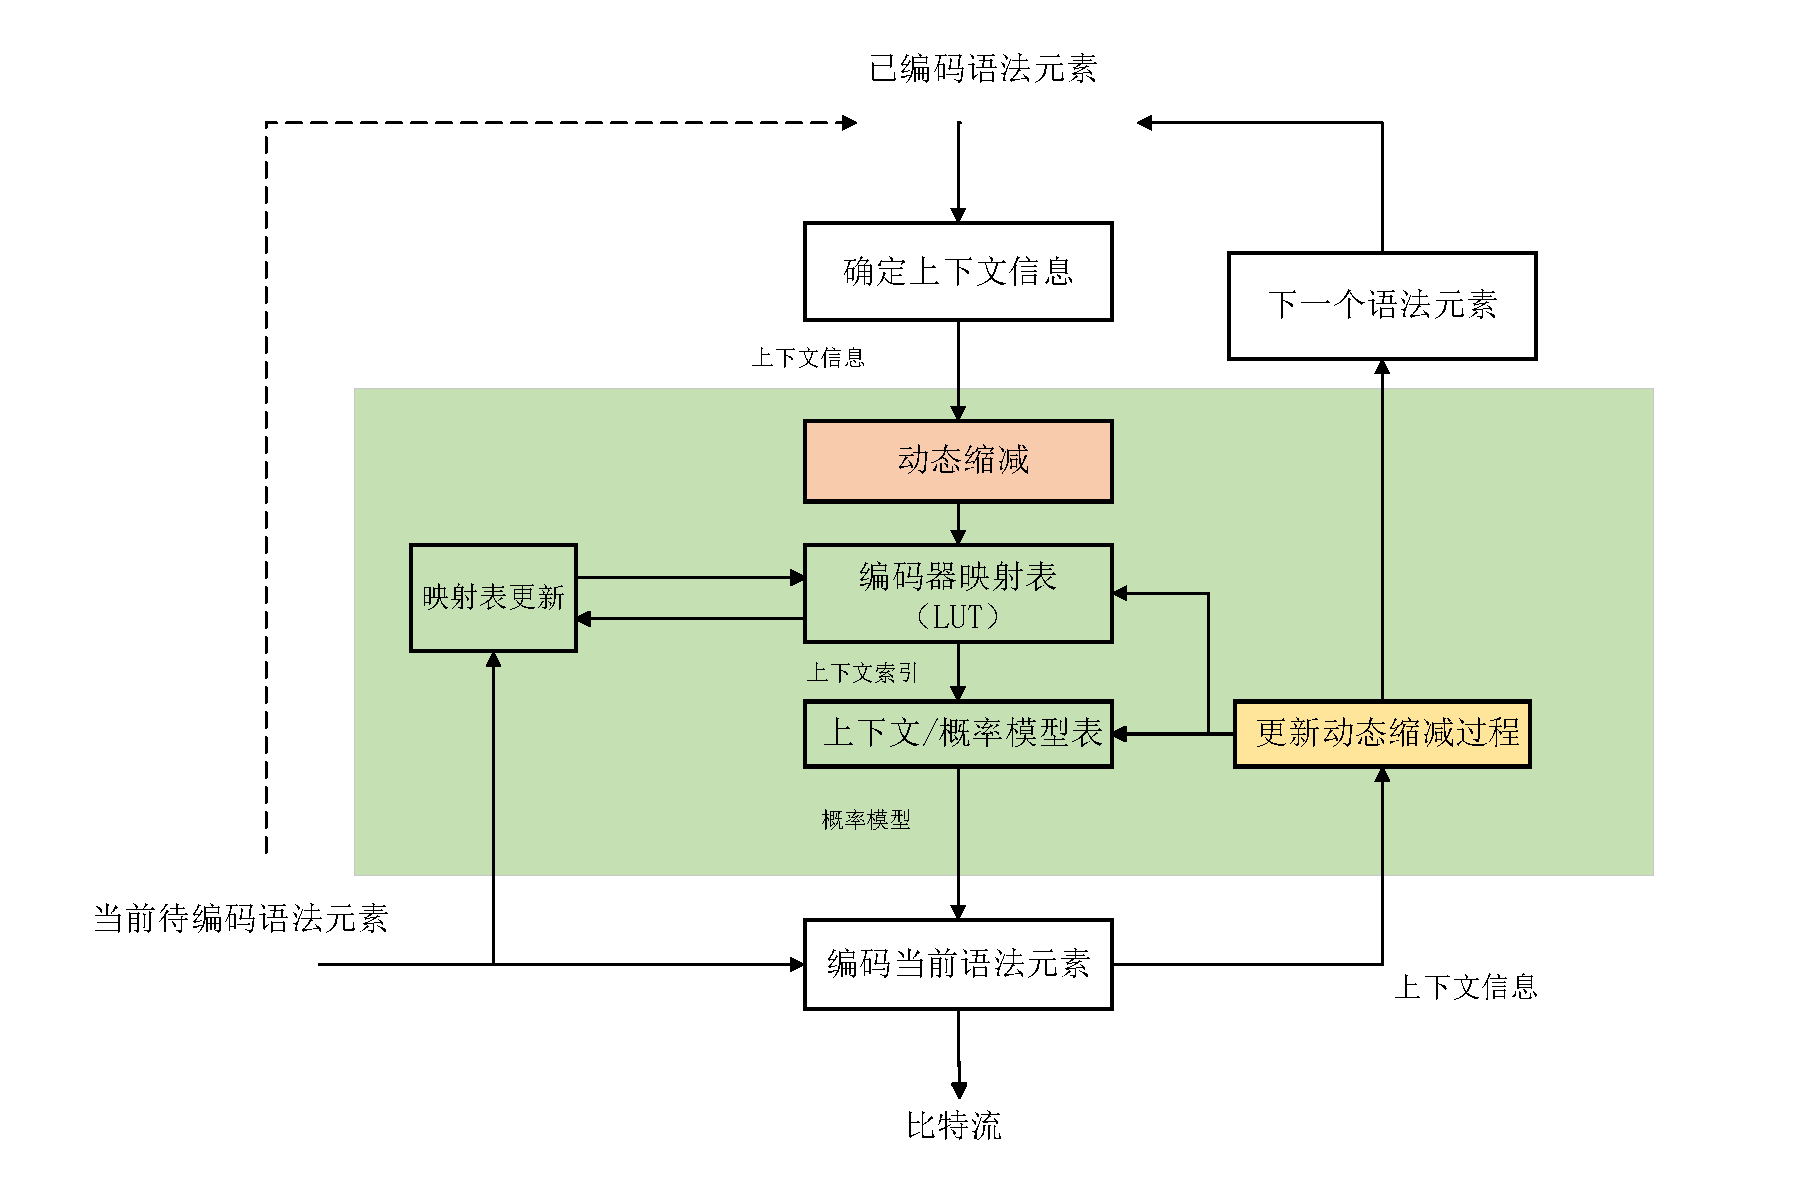
\includegraphics[scale=0.4]{image/动态OBUF流程图ykv2.pdf}
    \caption{动态OBUF流程图}
    \label{fig:动态OBUF流程图}
\end{figure}

动态OBUF相比于OBUF不同之处在于它将上下文信息分为了主要信息(Primary Information)和次要信息(Second Information),其中主要信息以较少的bit数承载着强相关的上下文信息,主要信息是不会随着熵编码的不断进行而减少的;次要信息的使用是动态OBUF的特点所在,图中标识的部分具体细节如图\ref{fig:dynamicreduction示意图}与\ref{fig:updatedynamicreduction示意图}所示。
\begin{figure}[h]
    %是可选项 h表示的是here在这里插入,t表示的是在页面的顶部插入
    \centering
    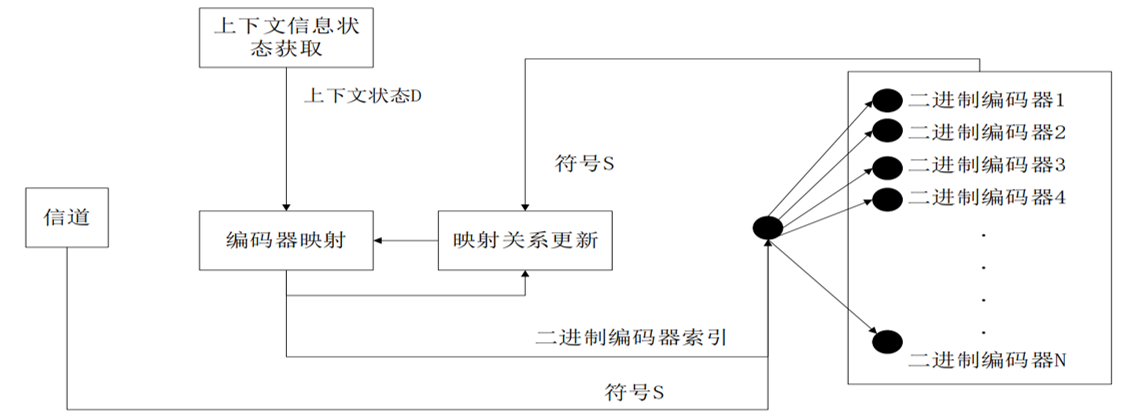
\includegraphics[scale=0.5]{image/OBUF工作原理图.png}
    \caption{OBUF工作原理图}
\end{figure}

动态减少是针对次要信息进行的,整个动态减少的过程主要由计数器N(i1,i2’)和决定次要信息使用bit位数的K两个参数控制,其中N(i1,i2’)是记录整个编码过程访问当前上下文的次数,当计数器超过一定的阈值$th$时,如图\ref{fig:updatedynamicreduction示意图}所示,首先DRn将会更新为DRn+1,这同样与熵编码器的索引表(LUT)相适应,最后还需要将计数器置零。另外,次要信息可以表示为${\rm{i}}2 = {\beta _{_1}}{\beta _2} \ldots {\beta _{\rm{k}}}$,通过更新K值,再对次要信息进行移位操作,便可达到动态更新次要信息的效果。

这样设计的目的在于,在编码初期,熵编码只会使用到很少的次要信息甚至仅使用主要信息就可以高效率的将待编码语法元素编码完成,因此大大节省了熵编码的bit流,提高了编码效率。
\begin{figure}[htb]
    %是可选项 h表示的是here在这里插入,t表示的是在页面的顶部插入
    \centering
    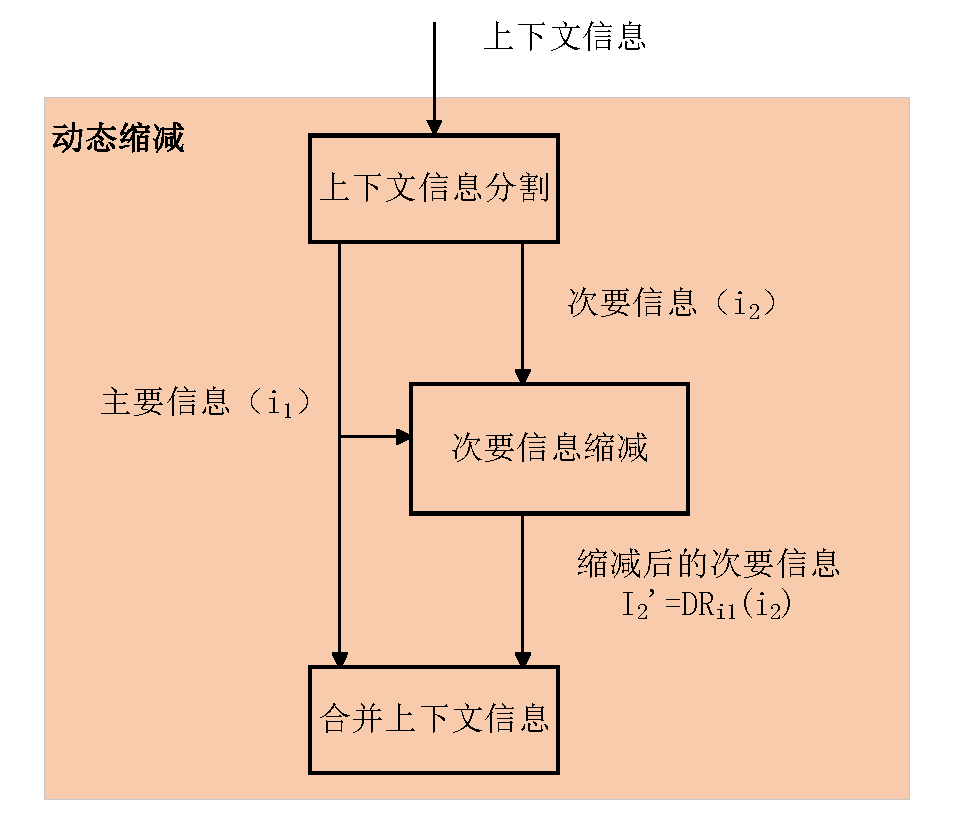
\includegraphics[scale=0.4]{image/动态缩减_crop.pdf}
    \caption{dynamicreduction示意图}
    \label{fig:dynamicreduction示意图}
\end{figure}
\begin{figure}[htb]
    %是可选项 h表示的是here在这里插入,t表示的是在页面的顶部插入
    \centering
    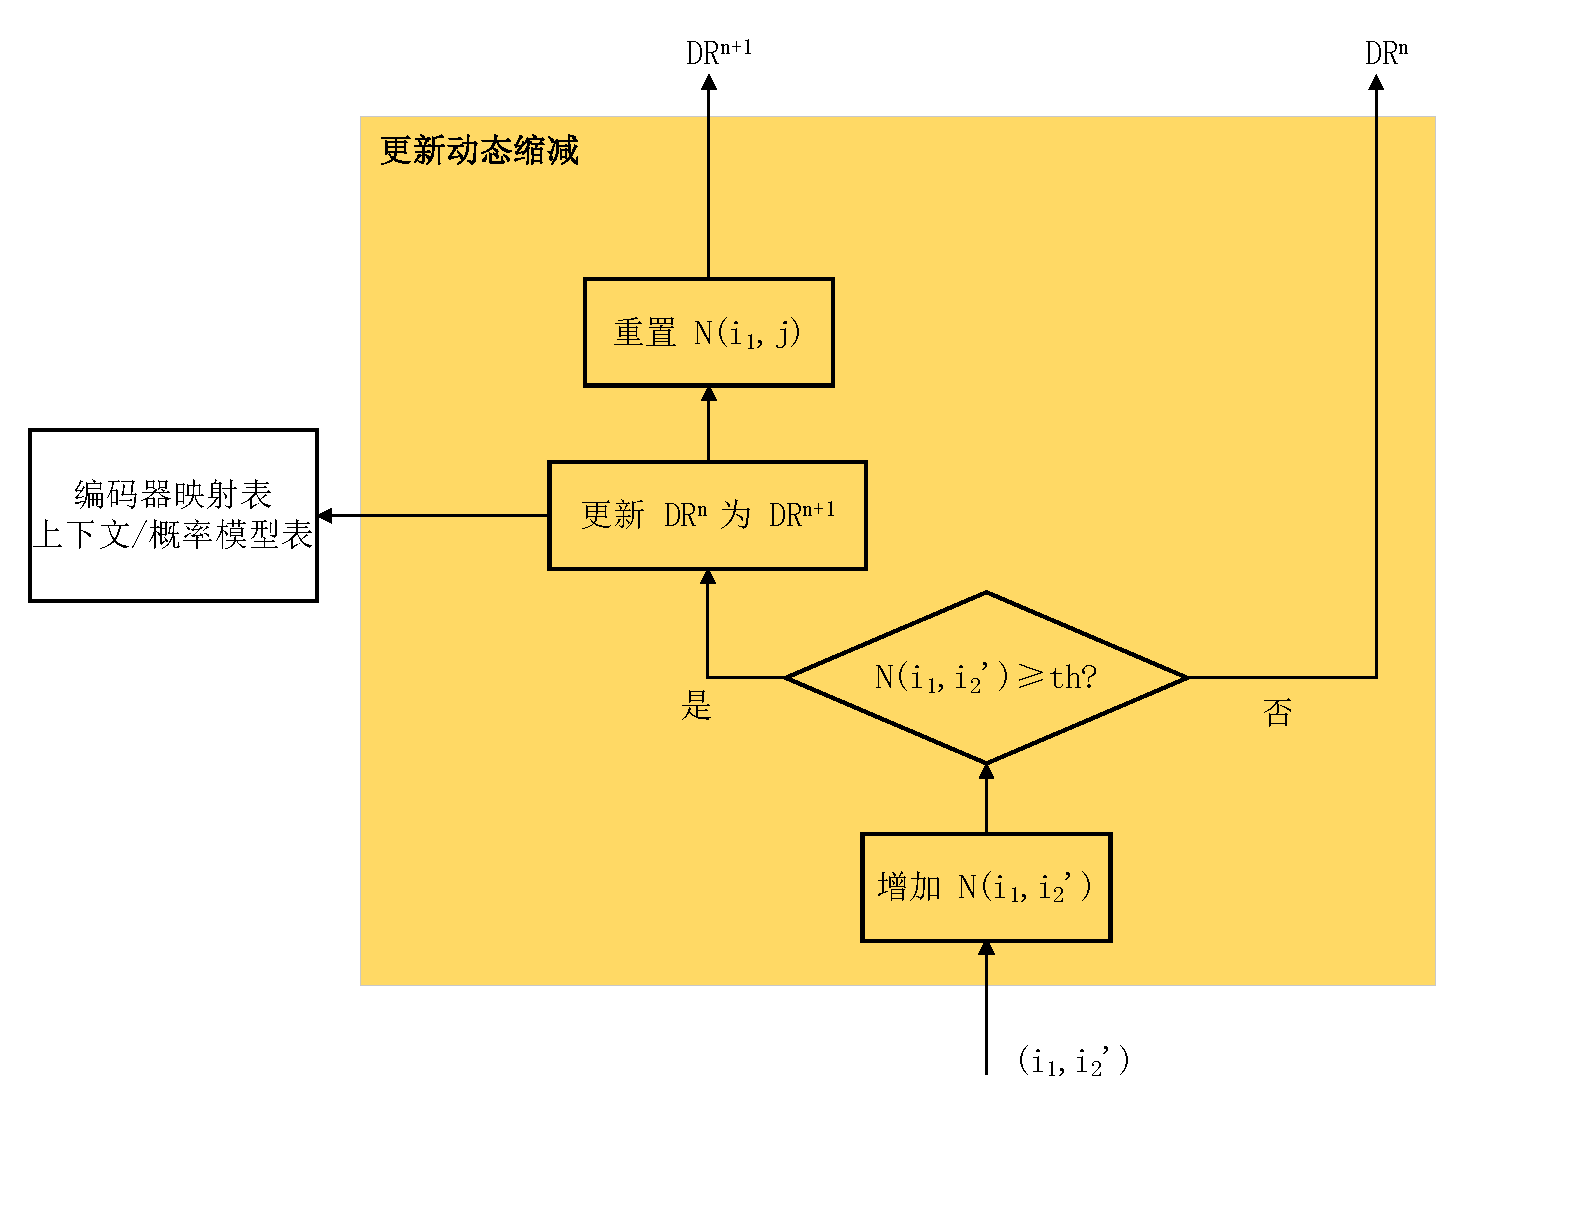
\includegraphics[scale=0.3]{image/更新动态OBUF_crop.pdf}
    \caption{updatedynamicreduction示意图}
    \label{fig:updatedynamicreduction示意图}
\end{figure}

\section{属性信息编码}
\label{sec:organization}
由图\ref{fig:编解码流程图}可以直观的看出,G-PCC主要包括两种属性变换编码方法,第一种是基于插值的带更新/提升的分层最近邻预测(Lifting Transform),第二种是区域自适应分层变换(RAHT)。其中,与Trisoup几何编码方法配合使用的主要是第二种。另外,这两种变换编码方式通常用于第一类点云数据。
\subsection{颜色变换}
G-PCC提供了颜色空间转换的功能,方便在不同场景下,应用合适的颜色空间。例如从RGB到YUV的颜色空间转换,具体公式如下所示:
\begin{equation}
    \left\{\begin{array}{c}
        Y=0.2126 \times R+0.7152 \times G+0.0722 \times B       \\
        U=-0.114572 \times R-0.385428 \times G+0.5 \times B+128 \\
        V=0.5 \times R-0.454153 \times G-0.045847 \times B+128
    \end{array}\right.
\end{equation}

转换的逆过程有:
\begin{equation}
    \left\{\begin{array}{c}
        R=Y+1.5748 \times(V-128)                        \\
        G=Y-0.18733 \times(U-128)-0.46813 \times(V-128) \\
        B=Y+1.85563 \times(U-128)
    \end{array}\right.
\end{equation}

其中,在整个颜色转换的过程中,使用的所有数据都是浮点型的,但是标准定义的输出结果统一转换为$unit8_t$格式,因此经过颜色空间转换后,颜色信息会产生一定的偏差,这也就限定了颜色空间转换只适应于属性有损条件下进行。

\subsection{属性转换}
进行属性信息编码前,因为当几何编码是有损时,重建出来的点云坐标位置与原始几何坐标有偏差,所以重建的点云没有属性信息,这个时候需要将原始的属性信息进行属性转换,为点云重新着色,同时需要保证属性失真最小。目前,在TMC13中,可以通过计算原始点云值多个近邻的距离加权平均数来实现属性转换。具体的属性转换过程如下:

1、为重建点云$(\widehat{X}_{i})_{i=0 \ldots  N_{r e c}-1}$建立起KD-Tree,将三个维度中的最长边方向作为划分主轴,其次基于划分主轴方向对重建点云进行划分。然后遍历原始点云的每个点,在重建点云KD-Tree结构中进行最近邻居点$Ref1$查找。由于是遍历的原始点云,因此最近邻居点会出现两种情况,一种是在重建点云中某个点作为原始点云中多个点的最近邻居点;第二种是原始点云中所有点都不会将某个重建点作为最近邻居点。

2、对原始点云$(X_{i})_{i=0\cdots N-1}$建立起KD-Tree,将三个维度中的最长边方向作为划分主轴,其次基于划分主轴方向对重建点云进行划分。然后遍历重建点云中的每个点,在原始点云KD-Tree结构中进行最近邻居点$Ref2$查找。但是由于是遍历重建点云的每一个点,每重建点都会找到一个原始点云作为其最近邻居。

3、首先判断$Ref1$集合是否为空,如果为空,则当前重建点的属性信息由相应索引的$Ref2$得到,否则当前重建点的属性由公式可得:
\begin{equation}
    \hat{A}_{i}=\frac{1}{num} \sum_{k=1}^{Ref(i)} A_{k}(i)
\end{equation}

\subsection{RAHT变换编码}
在八叉树划分的结构下,相邻节点里的属性值可能会比较相近,即这些属性信号的交流分量几乎为0,能量主要集中在直流分量上,通过变换将原始属性值转换成对应的AC,DC系数,就可以更好的对信号进行压缩去冗余。在GPCC中RATH变换\cite{ref21}主要过程如下:

1.构建和解析树

开始构建树时,需要对点云中所有的点按照莫顿序逐次进行扫描,通过莫顿码右移,不断将点云序列中的点进行合并,从而逐层构建树。在构建树的过程中,每个点的初始权重$weight_{org}$设置为1,初始颜色属性为$Attr_{org}$,每当两个点进行合并时,合并后点的属性值和权重分别为:
\begin{equation}
    Attr_s=Attr_{org1}+Attr_{org2}
\end{equation}
\begin{equation}
    weight_s=weight_{org1}+wieght_{org2}
\end{equation}

不断进行莫顿码右移和迭代,直至整个点云序列中只有一个点。解析树的过程是构建树的相反过程,基本规则相同。

2.预测和变换

由于最高级父块处于树的顶部位置,并没有可以用于参考从而进行预测的父块或者祖父块,因此第n-1到n-4层不进行预测,当预测标识开启时,除第一级父块外的其余层都会进行预测。通过occupancy标记当前父节点中8个子节点的占用情况。通过父级块对当前块进行预测,首先要寻找当前块的父块的19(1+6+12)个邻居节点,其中,1为邻居节点是当前块的父节点,6为与父节点共面的邻居节点,12为与父节点共线的邻居节点,但这19个邻居节点不一定总是被占据,所以需要对邻居节点进行标识,用“1”表示当前子节点被占据,用0表示当前子节点不被占据,邻居节点示意图如 \ref{fig:邻居节点的示意图} 所示:
\begin{figure}[h]
    %是可选项 h表示的是here在这里插入,t表示的是在页面的顶部插入
    \centering
    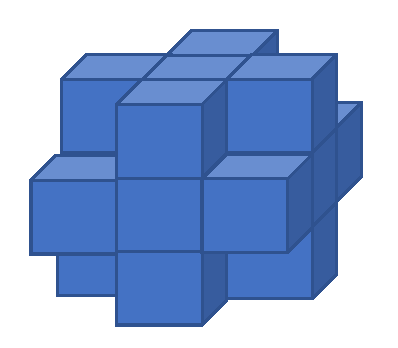
\includegraphics[scale=0.7]{image/邻居节点示意图v2.pdf}
    \caption{邻居节点的示意图}
    \label{fig:邻居节点的示意图}
\end{figure}

查找完邻居节点后,就需要对子节点进行预测。不同类型的邻居节点,在预测中所占的权重是不一样的。首先是父节点对子节点预测效果最好,其次是共面的父邻居节点,再者是共线的父邻居节点。因此在设置预测权重时,权重值依次递减。

对属性信息和预测的属性信息进行RAHT变换,根据构造的树的结构,从最高层开始,每三层进行RAHT变换,其中每个父块作为变换块来依次进行RAHT变换。
如果进行在该层进行预测,则需要对属性信息和预测属性信息都进行RAHT变换;如果不进行预测,则只需要对属性信息进行RAHT变换。用$w_1$和$w_2$分别表示两个待变换块包含的点数,用$c_1$和$c_2$表示两个待变换块的属性值,则RATH变换公式如\ref{fig:RAHT公式1}和\ref{fig:RAHT公式2}所示:
\begin{equation}
    \mathrm{RAHT}\left(w_{1}, w_{2}\right)=\frac{1}{\sqrt{w_{1}+w_{2}}}\left[\begin{array}{cc}
            \sqrt{w_{1}}  & \sqrt{w_{2}} \\
            -\sqrt{w_{2}} & \sqrt{w_{1}}
        \end{array}\right]
    \label{fig:RAHT公式1}
\end{equation}

\begin{equation}
    \left[\begin{array}{l}
            D C \\
            A C
        \end{array}\right]=\mathrm{RAHT}\left(w_{1}, w_{2}\right)\left[\begin{array}{l}
            c_{1} \\
            c_{2}
        \end{array}\right]
    \label{fig:RAHT公式2}
\end{equation}
其中DC系数为属性的加权平均值,AC系数为相邻两点的属性残差。计算AC系数的残差,计算公式如\ref{fig:RAHT公式3}所示:
\begin{equation}
    Attr _ {res }=  AttrCoff_{org} -  AttrCoff_{pred }
    \label{fig:RAHT公式3}
\end{equation}

若当前层不进行预测,则直接对属性信息变换系数进行量化和熵编码。若当前层需要进行预测时,对上述步骤得到的AC系数的残差进行量化和熵编码。

\subsection{Lifting预测变换编码}
该方法利用点云中已编码点的属性值对待编码点进行预测,从而得到待编码点的属性预测值,并将待编码点的真实属性值与预测值相减得到预测残差,以达到去除空域冗余的目的。基于莫顿码排序选取预测点,一定程度上反映了空间近邻的相关性,但是由于存在空间跳跃点等情况,预测效果并不是很好。因此引入了LOD (Level Of Detail) 划分技术\cite{ref20},也就是将点云划分成不同的层次结构,利用层次结构对属性进行有效预测。

LOD 划分有三种方法,包括基于距离的 LOD 划分、基于采样率的 LOD 划和基于八叉树的 LOD 划分。如图 \ref{fig:10} 所示,基于距离的 LOD 划分适用于稠密均匀的点云,如 cat1类型;基于采样率的 LOD 划分适用于分布稀疏不均匀的点云,如 cat3-frame 和 cat3-fused 类型;基于八叉树的 LOD 划分适用于 scalable 情况,对齐几何和属性的点数,使其与几何八叉树结构对齐。

Lifting 变换编码是一种依赖于多层LOD的属性编码方式,也就是将点云划分成不同的层次结构,利用层次结构对属性进行有效预测。其主要包含了分割、预测、更新三个部分,如图\ref{fig:提升变换流程图}所示。
\begin{figure}[h]
    %是可选项 h表示的是here在这里插入,t表示的是在页面的顶部插入
    \centering
    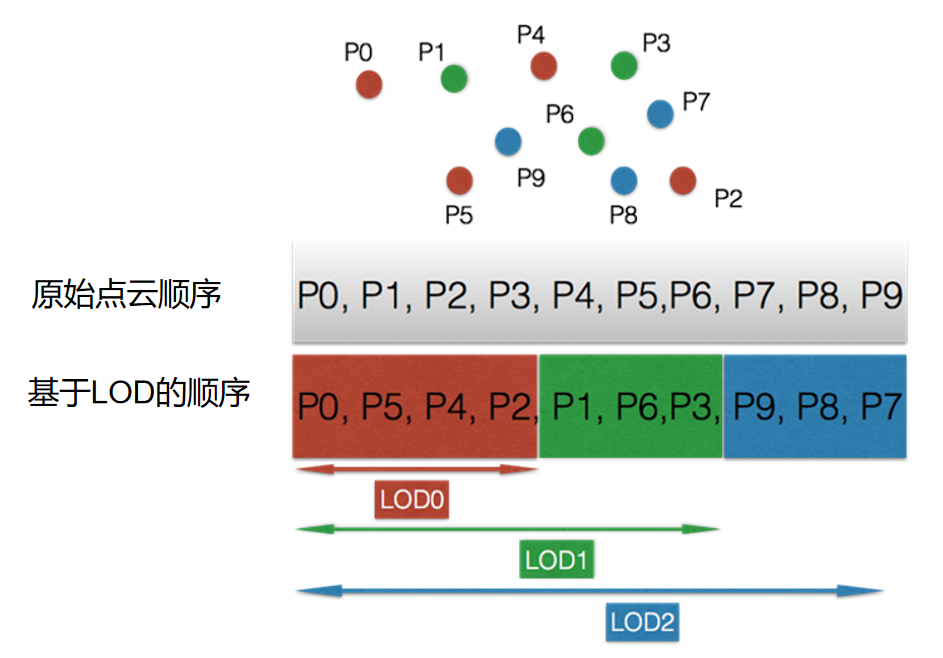
\includegraphics[scale=0.3]{image/LOD.png}
    \caption{基于距离的LOD划分示意图}
    \label{fig:10}
\end{figure}

\begin{figure}[h]
    %是可选项 h表示的是here在这里插入,t表示的是在页面的顶部插入
    \centering
    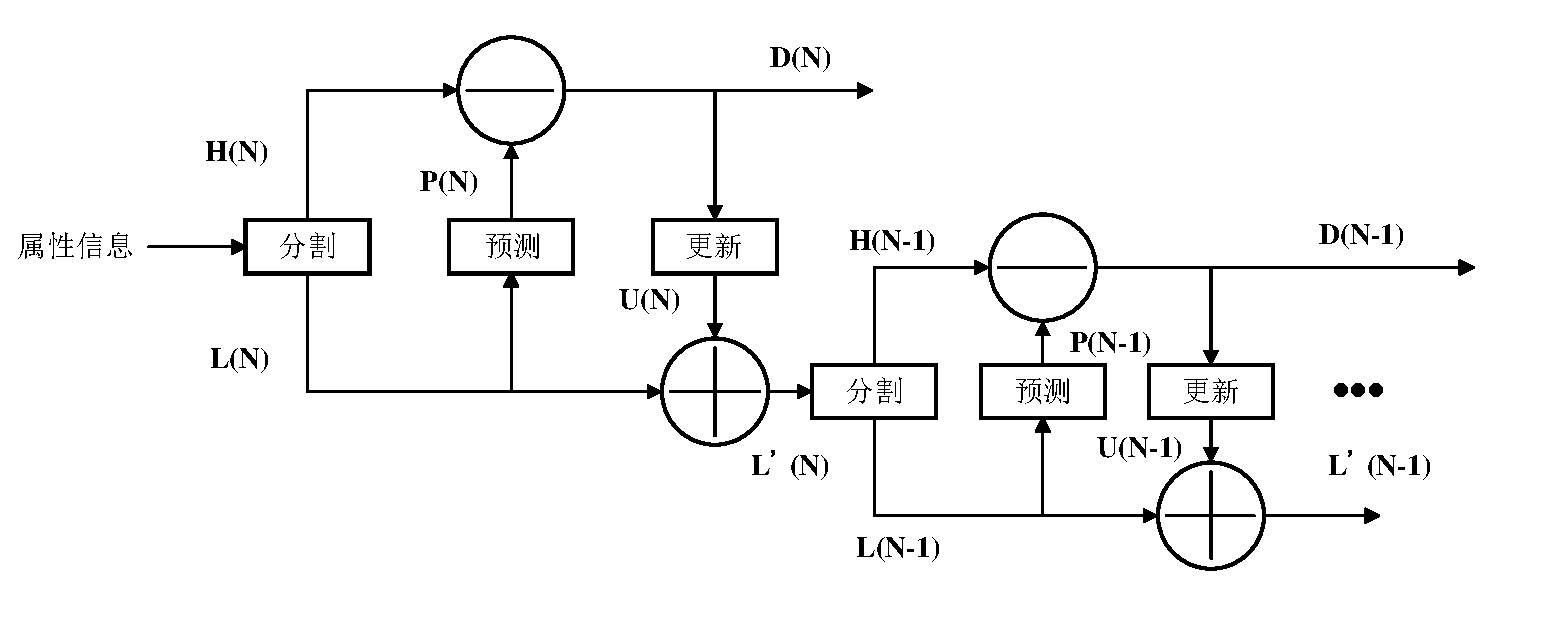
\includegraphics[scale=0.5]{image/提升变换流程图v2.pdf}
    \caption{LOD划分示意图}
    \label{fig:提升变换流程图}
\end{figure}

其中,$H(N)$表示高层次点云是与细化层相关的属性集,$L(N)$表示低层次点云是与$LOD(N)$相关的属性集,$D(N)$表示预测残差。

Lifting变换建立在分层预测的基础上,引入了权重更新和自适应量化的概念。低层 LOD 层被频繁的用来预测高层 LOD 层中的点,所以更新量化权重的目的是给低层 LOD 层点云提升一定的权重值来表征其重要性,使其影响更大,量化损失更小,预测结果更准确。Lifting 变换的关键在于预测和更新算法。预测算法得到的预测残差是变换过程中的高频分量,而通过更新算子来提升的属性信息是输入信号的低频分量。低频分量表征了点云属性的基本特征,反映出点云属性的整体情况,高频分量表征了点云属性的更多细节特征。Lifting 变换运算时间短,占用存储少,可准确地将点云属性划分为低频和高频两个部分,具有良好的压缩性能和重建效果

\section{评价标准}
\label{sec:suborganization}
评价一个点云压缩算法的性能好坏一般从三个方面出发:

1、编解码前后点云失真情况,具体又细分为几何失真与属性失真。两部分的失真计算都是基于对应点的,几何失真计算的是几何距离的失真,属性失真计算的是属性数值的失真。其中对应点就是原始点云的点在重建点云中的最近邻居点或者重建点云中的点在原始点云中的最近邻居点。

2、编码后比特流的大小。比特流大小可以通过 Bpip(bits per input point,即平均每个输入点所用比特数)来衡量,Bpip 越小,压缩性能越好。

3、编解码点云的时间复杂度。时间复杂度可以通过编解码过程耗费的时间来衡量,时间越短,压缩性能越好。

在无损压缩情况下,不存在点云的失真,只要考后两个方面来衡量性能。在有损压缩的情况下,点云的失真程度也是重要的考量,在衡量性能时三个方面都要考虑。在实际评估过程中,可从 rate 模式和 PSNR 模式两方面进行比较。BD-rate 为负值时,表示相同 PSNR 的条件下,码率减小,性能提升;BD-PSNR为负值时,表示相同码率的条件下,PSNR 增大,性能提升。


\ifx\allfiles\undefined
\end{document}
\fi
%%% Local Variables:
%%% TeX-master: "thesis-doctor.tex"
%%% End:
%% ----------------------------------------------------------------------
%%% END OF FILE 
%% ----------------------------------------------------------------------
%% ----------------------------------------------------------------------
%% START OF FILE
%% ----------------------------------------------------------------------
%% 
%% Filename: ch02-options.tex
%% Author: Fred Qi
%% Created: 2012-12-26 09:15:56(+0800)
%% 
%% ----------------------------------------------------------------------
%%% CHANGE LOG
%% ----------------------------------------------------------------------
%% Last-Updated: 2015-05-14 20:48:32(+0300) [by Fred Qi]
%%     Update #: 77
%% ----------------------------------------------------------------------
\ifx\allfiles\undefined
\documentclass[bachelor,print,msfonts]{xduthesis}

% 这里是可能用到的其他宏包,根据自己论文撰写的需要添加
\usepackage{listings}
\usepackage{overpic}
\lstset{language=TeX, basicstyle=\ttfamily}

\newcommand{\figref}[1]{图\ref{#1}}
\newcommand{\sArt}{state-of-the-art}
\newcommand{\wyh}[1]{{\textcolor{blue}{#1}}}
\newcommand{\secref}[1]{Sec. \ref{#1}}
\newcommand{\tabref}[1]{Tab.~\ref{#1}}
\newcommand{\thudot}[1]{} % thubib.bst 定义每条参考文献最后的点\thudot
\graphicspath{{./}{./img/}{./fig/}{./image/}{./figure/}{./picture/}}
\newcommand{\bs}{\boldsymbol}
\usepackage{float}
\setcounter{chapter}{1}

\begin{document}
\mainmatter
\fi

\chapter{Trisoup顶点标识与位置信息的熵编码优化}
\label{cha:options}
Trisoup几何信息编码算法中对顶点标识信息和位置信息需要进行编码操作,由于点云空间位置存在一定相关性,采用普通算数编码会编码很多冗余信息。因此Trisoup对顶点信的息编码采用了如本文\ref{动态OBUF}所述的动态OBUF的熵编码方法,一定程度上消除了点云空间位置上的相关性,进一步压缩了码流。然而,现有MPEG提出的编解码标准中为顶点标识信息与顶点位置信息构建的上下文未必是最佳。为此,本章通过对各个上下文信息熵与条件熵的测量,依照熵值越小,上下文信息越有效的原则,对现有上下文顺序进行了一定调整,以提高熵编码效率。
\section{Trisoup几何信息熵编码的上下文}
在TMC13v20版本的参考代码中,MPEG采纳了由Sébastien提出的拓展Trisoup中上下文所用到的邻居数量的提案。截至目前,Trisoup在编解码顶点信息时将当前待编码边按照朝向的不同分为三种情况,分别为:平行于$x$轴、平行于$y$轴、平行于$z$轴。每条待编码边拥有各自的18条邻居边,但实际用于构建上下文的邻居边是按照不同朝向从18条边中选出的9条边,如图\ref{fig:邻居边示意图}所示。另外,由于上下文构建的需要,如果某一邻居边被占据,边上顶点位置在被量化为2bit的基础上再次细分出一个$closest$区间和$close$区间,用于组成上下文的信息除了选取的9条边占据情况外,还包括当前待编码边周围节点的占据情况,如图\ref{fig:上下文组成元素的具体含义示意图}所示。
\begin{figure}[htbp]
    %是可选项 h表示的是here在这里插入,t表示的是在页面的顶部插入
    \centering
    \subfloat[18条邻居边]{
        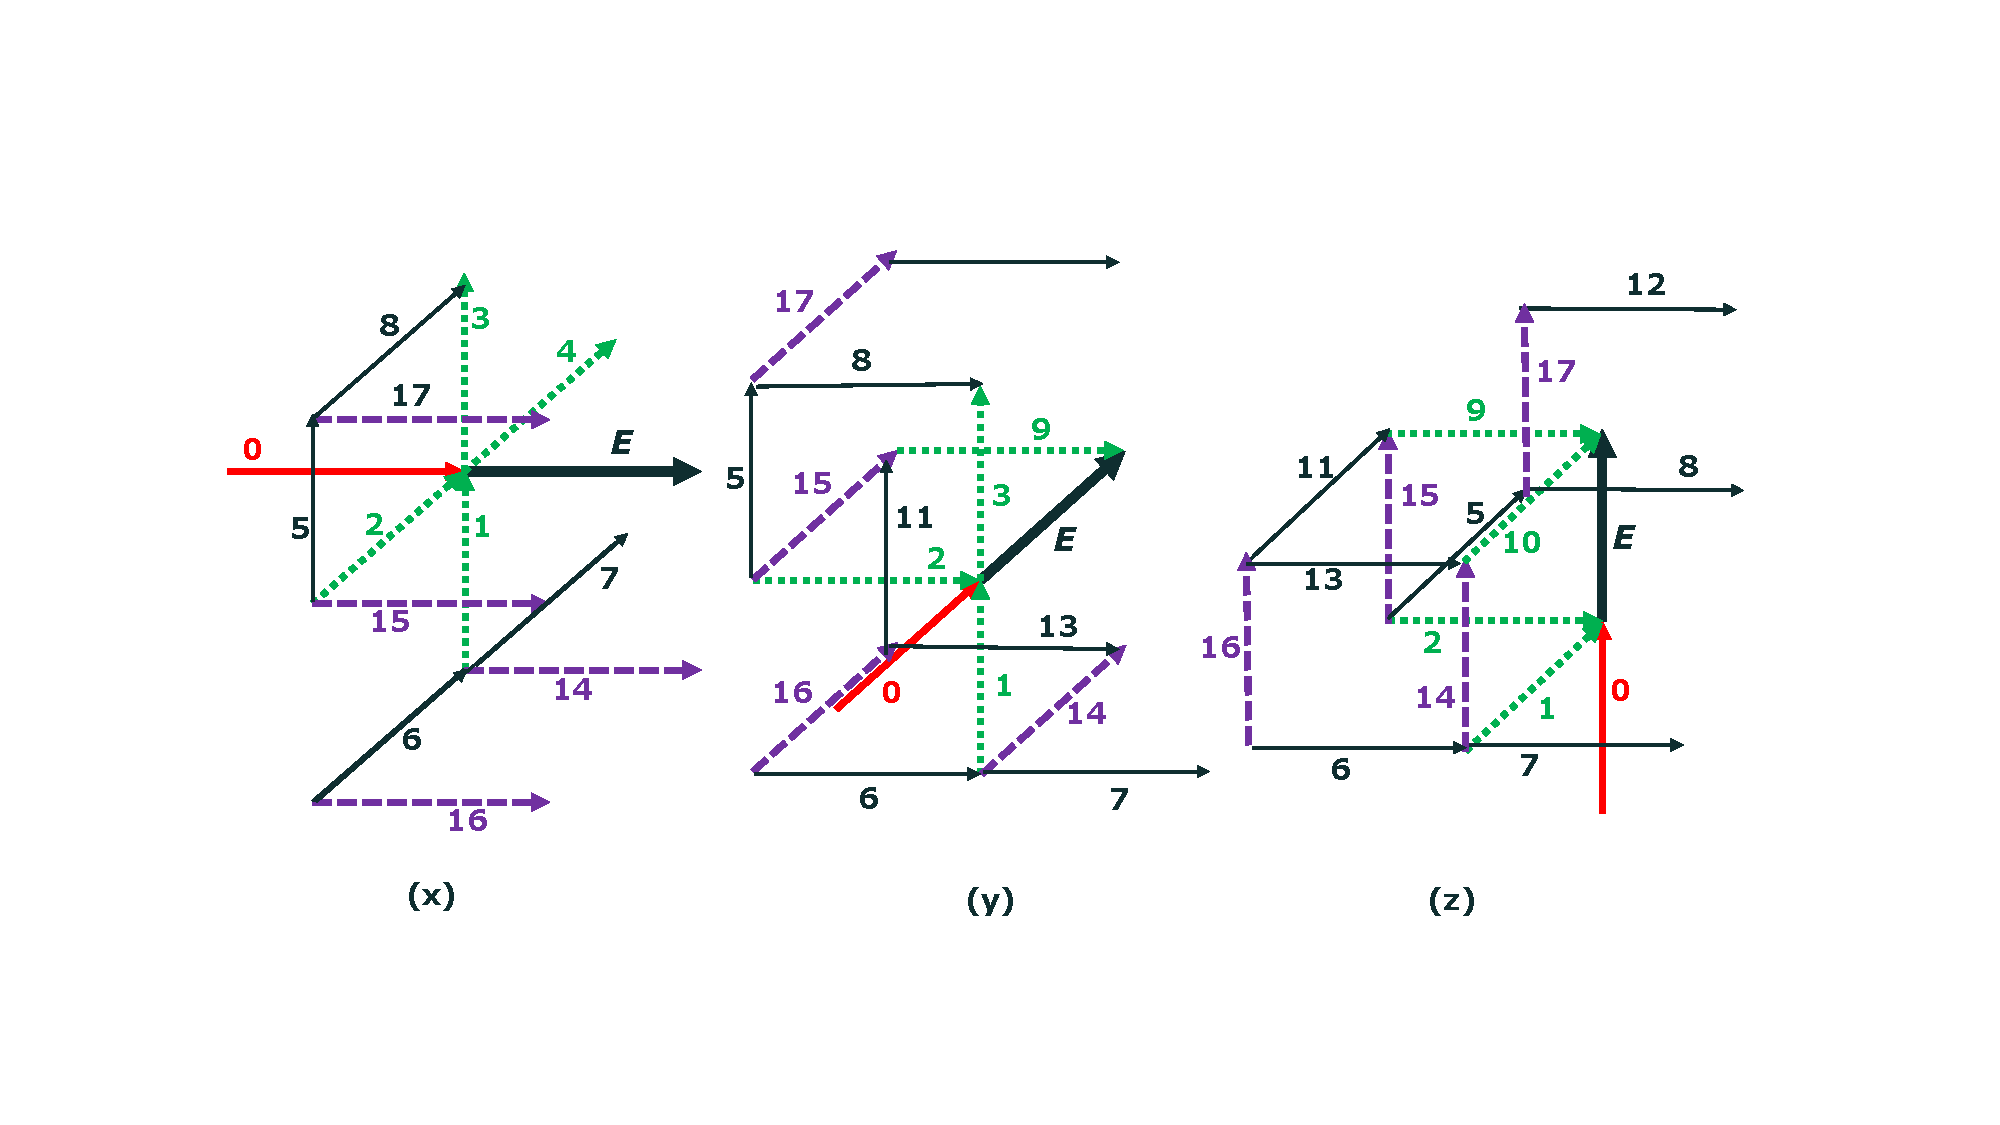
\includegraphics[scale=0.2]{image/18条边.pdf}
    }
    \hspace{0.1in}
    \subfloat[9条邻居边]{
        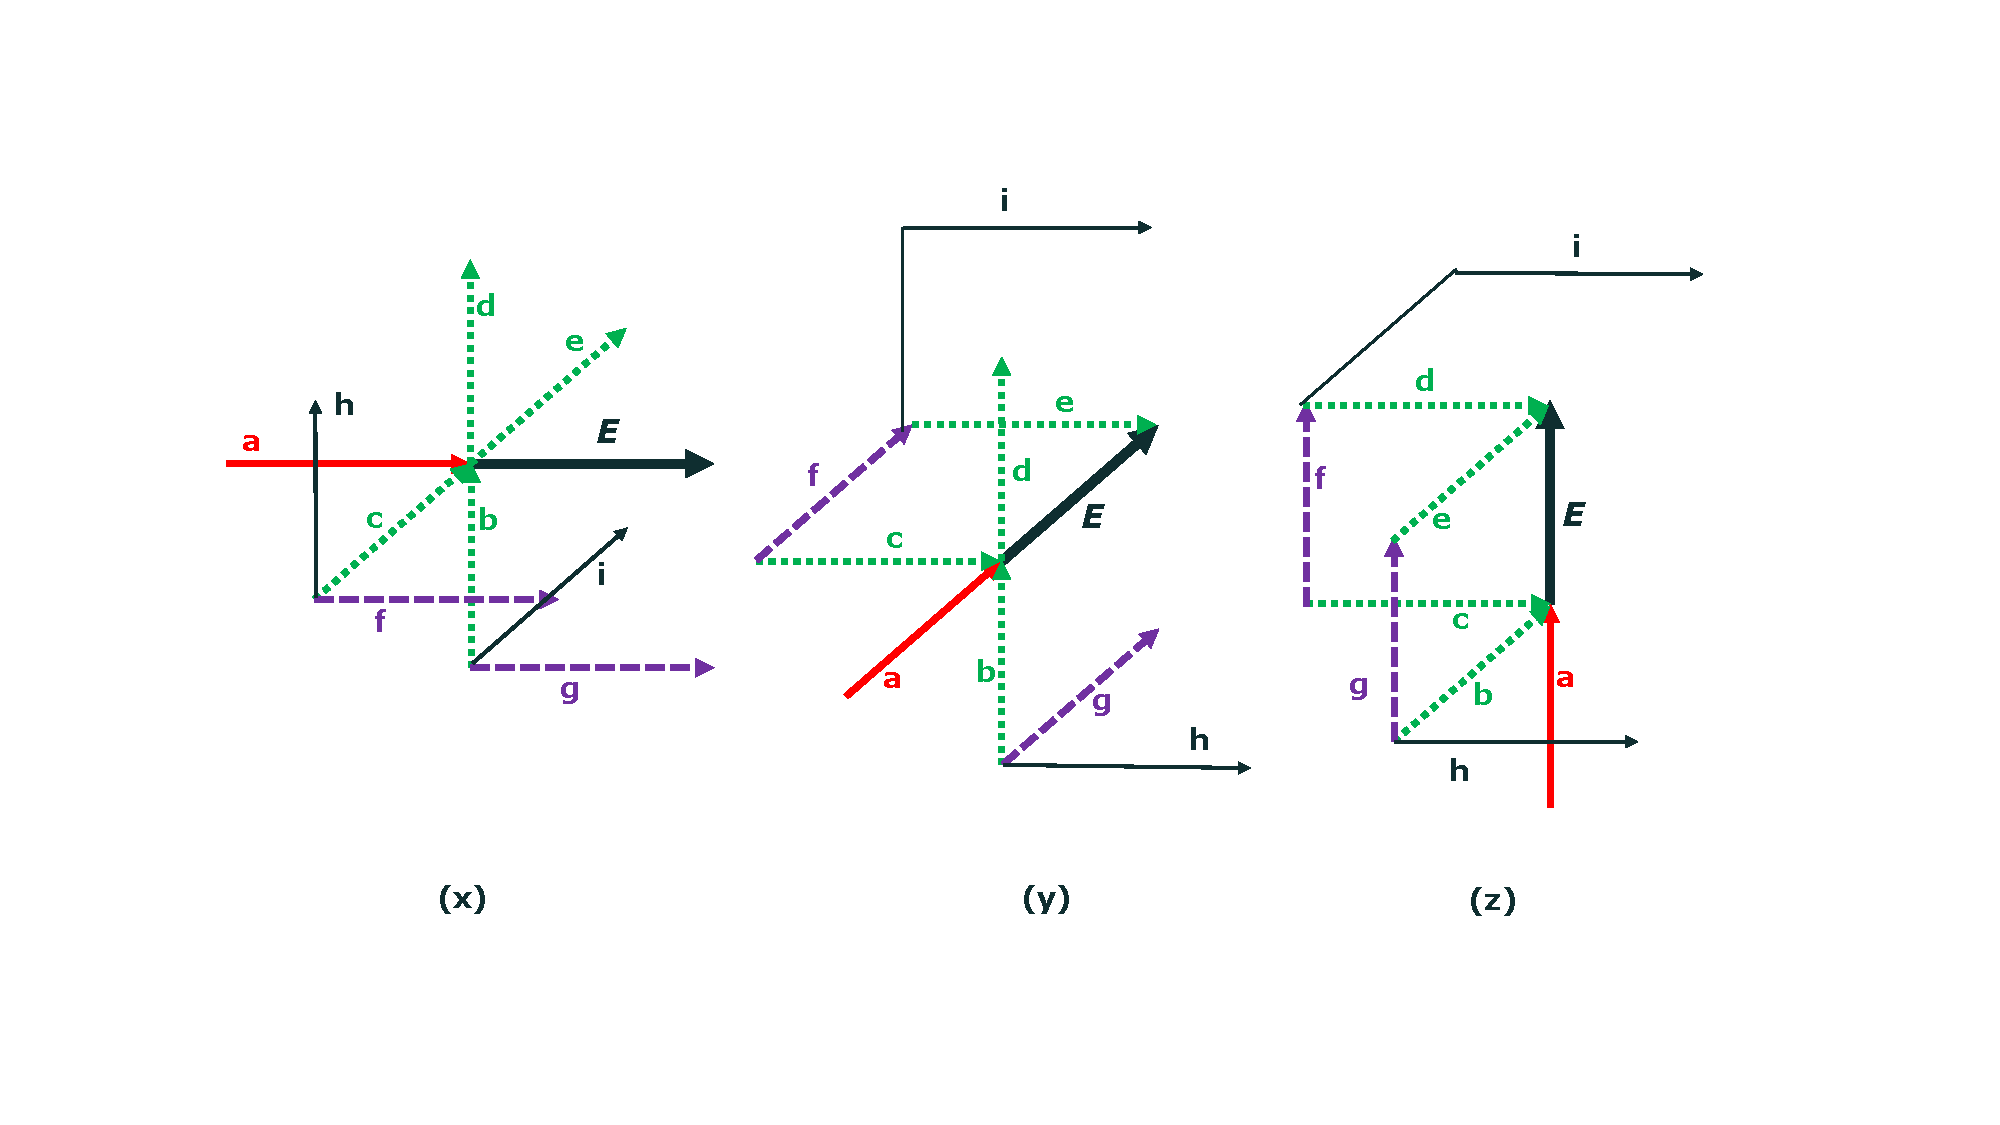
\includegraphics[scale=0.2]{image/9条边.pdf}
    }
    \caption{邻居边示意图}
    \label{fig:邻居边示意图}
\end{figure}
\\
\begin{figure}[htbp]
    %是可选项 h表示的是here在这里插入,t表示的是在页面的顶部插入
    \centering
    \subfloat[边的区间划分示意图]{
        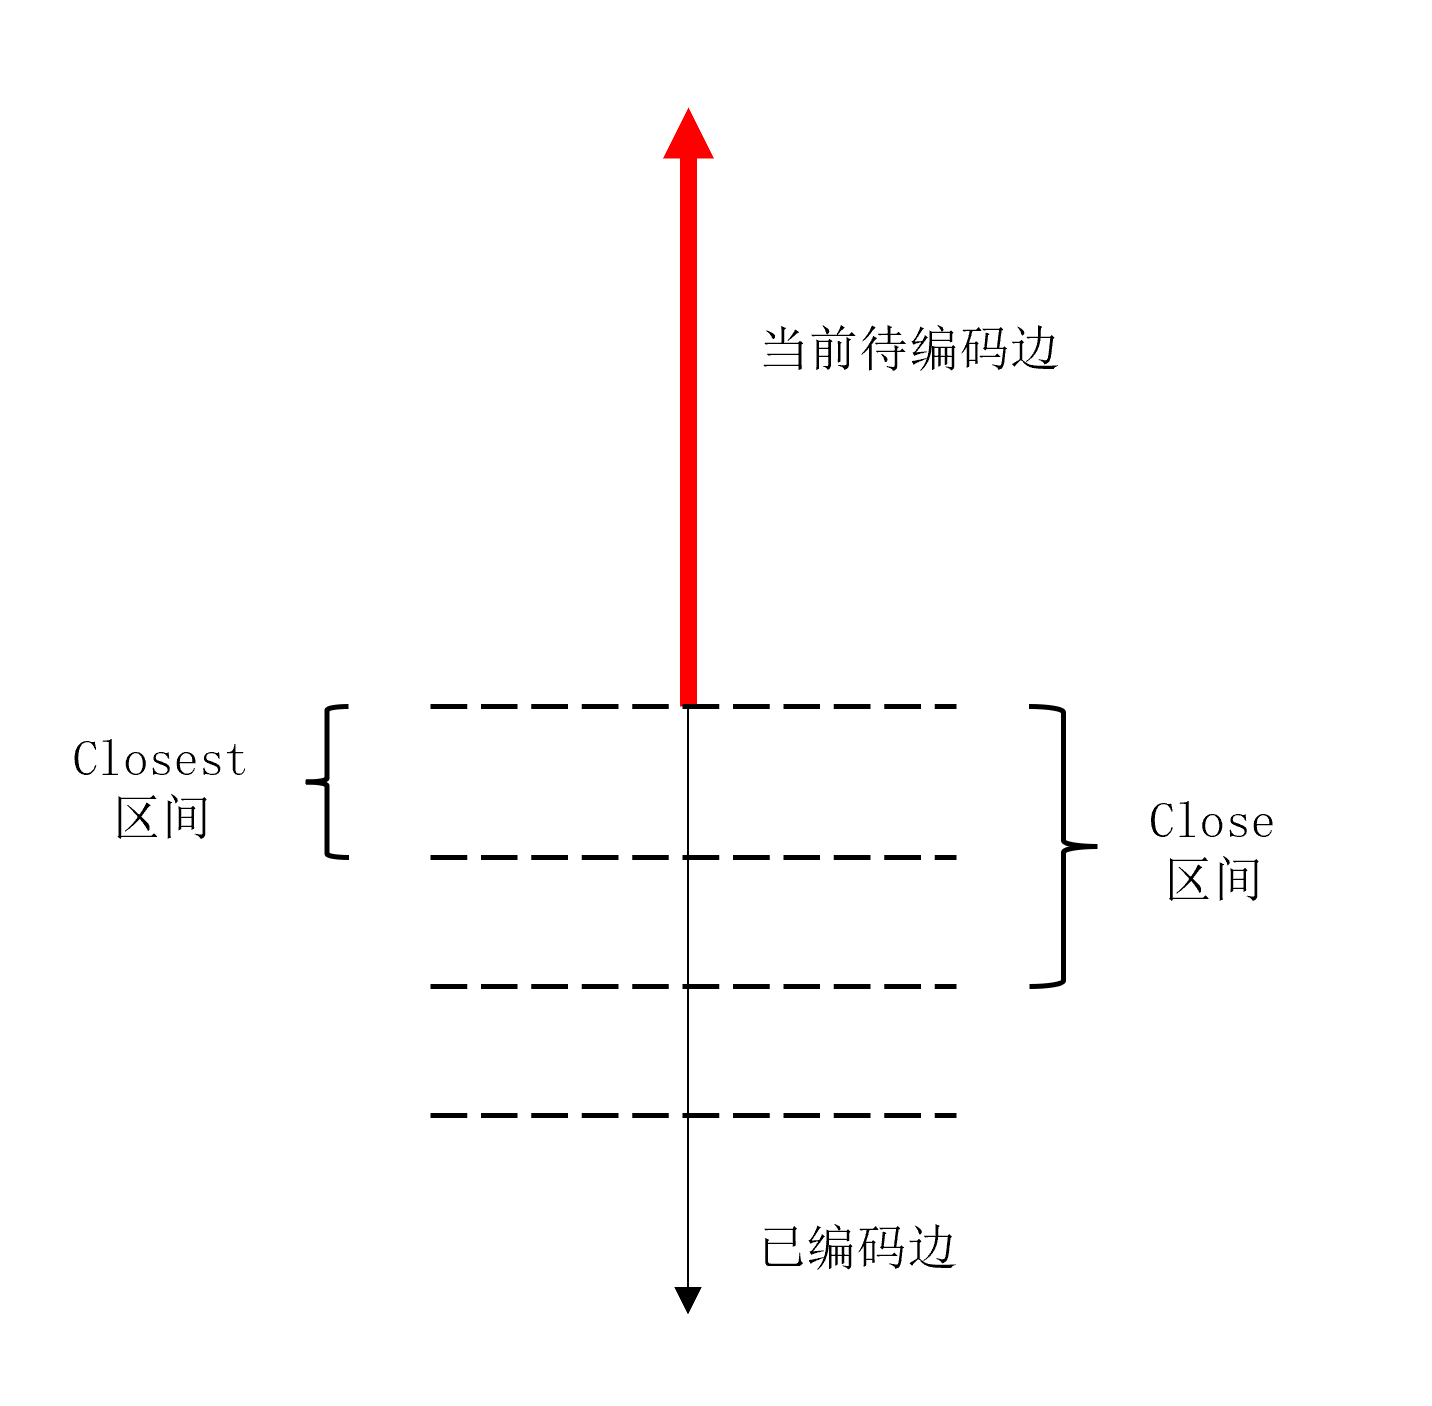
\includegraphics[scale=0.3]{image/区间划分示意图.png}
    }
    \hspace{0.2in}
    \subfloat[当前待编码边周围节点示意图]{
        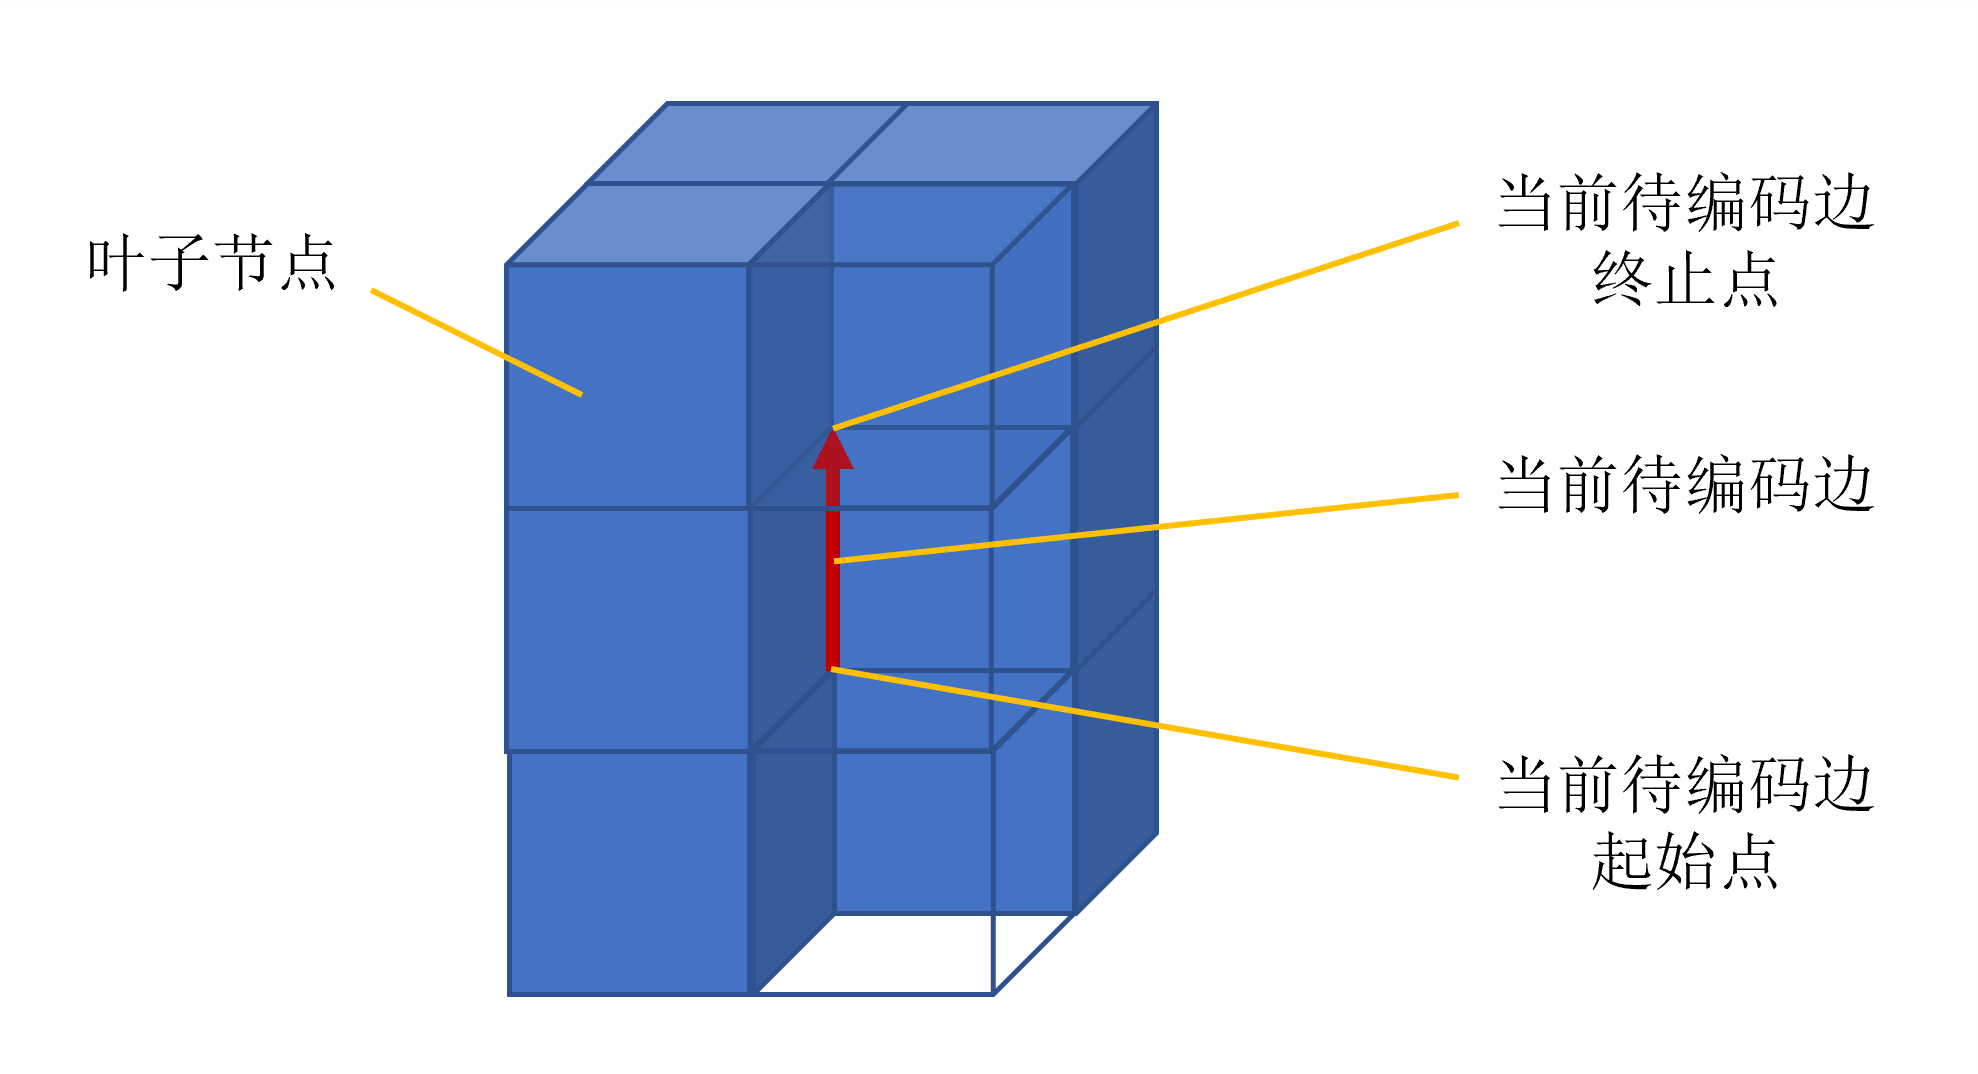
\includegraphics[scale=0.3]{image/当前待编码边周围节点.png}
    }
    \caption{上下文组成元素具体含义示意图}
    \label{fig:上下文组成元素的具体含义示意图}
\end{figure}

利用上述这些邻居边信息和邻居节点信息分别为编码顶点标识信息、顶点位置信息的高bit位以及顶点位置的低bit位构建了三套不同的上下文。其中强相关的信息作为上下文的主要信息,次相关的信息作为上下文的次要信息。
\begin{table}[h]
    \fontsize{10.5pt}{15pt}\selectfont
    \centering
    \caption{\label{tab1} 标识信息上下文编号}
    \begin{tabular}{cc}
        \toprule
        上下文名称                   & 编号 \\
        \midrule
        missedCloseStart             & ctx1 \\
        patternClosest  \& 1         & ctx2 \\
        direction                    & ctx3 \\
        patternClose \& (0b00011111) & ctx4 \\
        missedCloseStart             & ctx5 \\
        missedCloseStart             & ctx6 \\
        \bottomrule
    \end{tabular}
\end{table}

\subsection{顶点标识信息上下文}
顶点标识信息简而言之就是用1bit位来标识当前待编码边是否被占据,如果被占据则该bit置“1”,如果不被占据则该bit置“0”。其上下文结构如下:

1、主要信息组成
\begin{figure}[htbp]
    %是可选项 h表示的是here在这里插入,t表示的是在页面的顶部插入
    \centering
    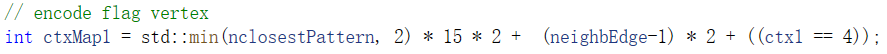
\includegraphics[scale=0.4]{image/flag主要信息组成.png}
    \caption{组成标识信息上下文的主要信息代码截图}
    \label{fig:flag主要信息组成}
\end{figure}

其中:

$nclosestPattern:$表示9条边中的前5条边在closest区间的数量。

$neighbEdge:$表示包含当前待编码边的 4 个节点的占据情况。

$ctx1:$表示包含当前待编码边起始点坐标的 4 个节点被占据的数量。
\\
\\
2、次要信息组成
\begin{figure}[htbp]
    %是可选项 h表示的是here在这里插入,t表示的是在页面的顶部插入
    \centering
    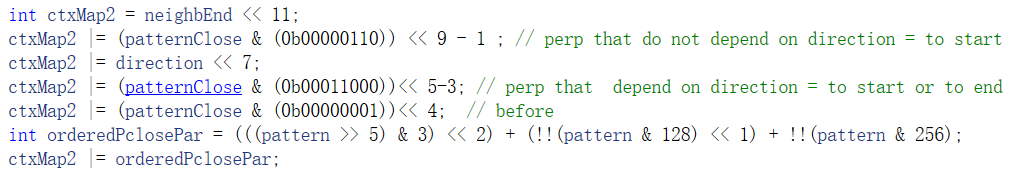
\includegraphics[scale=0.4]{image/flag次要信息组成.png}
    \caption{组成标识信息上下文的次要信息代码截图}
    \label{fig:flag次要信息组成}
\end{figure}

其中:

$neighbEnd$:表示包含当前待编码边终止点的 4 个节点的占据情况。

$patternClose$:9 条边在 close 区间被占据的情况。

$direction$:当前待编码边的朝向$(0=X,1=Y,2=Z)$。

$pattern$:9条边的被占据的情况。

另外,如表\ref{tab1}所示,本文按照次要信息的现有上下文顺序对其进行编号。

\subsection{顶点位置信息上下文}
在编码叶子节点中某一条被占据边上的顶点坐标时,首先需要对顶点坐标进行量化操作,现有的量化操作是将顶点坐标量化为0,1,2,3四个坐标值,因此需要用2bit来表示量化后的顶点位置信息。由于两个bit位所承载的位置信息在物理含义上不一致,对于高bit位,它将量化后的顶点坐标可选范围缩减一半,顶点坐标取值要么为0,1要么为2,3;低bit位则是在高bit位基础上,完全确定顶点坐标位置。因此分别为其构建不同的上下文模型。

对于高bit位:

1、主要信息组成

\begin{figure}[htbp]
    %是可选项 h表示的是here在这里插入,t表示的是在页面的顶部插入
    \centering
    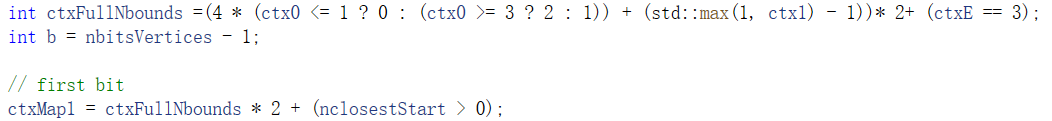
\includegraphics[scale=0.4]{image/position1主要信息组成.png}
    \caption{组成位置信息上下文高bit的主要信息代码截图}
    \label{fig:position1主要信息组成}
\end{figure}

其中:

$ctx0$:表示包含当前待编码边终止点坐标的 4 个节点被占据的数量。

$ctxE$:表示当前待编码边周围4各个节点被占据数量

$nclosestStart$:表示9条边中的前5条边在closest区间被占据的数量


2、次要信息组成

\begin{figure}[htbp]
    %是可选项 h表示的是here在这里插入,t表示的是在页面的顶部插入
    \centering
    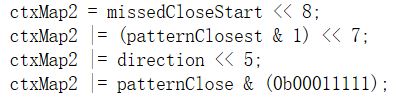
\includegraphics[scale=0.4]{image/position1次要信息组成.png}
    \caption{组成位置信息上下文高bit的次要信息代码截图}
    \label{fig:positon1次要信息组成}
\end{figure}

其中:

missedCloseStart:表示4条相邻垂直边不被占据的数量

patternClosest:表示9条边在closest区间被占据的情况

对于低bit位,其上下文模型的主要信息部分与高bit位一致,主要差别体现在次要信息更加丰富。下面给出该bit位上下文模型的次要信息组成:

\begin{figure}[htbp]
    %是可选项 h表示的是here在这里插入,t表示的是在页面的顶部插入
    \centering
    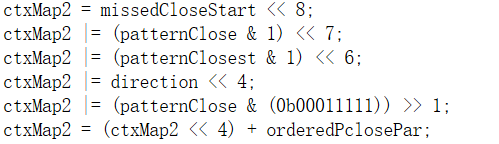
\includegraphics[scale=0.4]{image/position2次要信息组成.png}
    \caption{组成位置信息上下文低bit的次要信息代码截图}
    \label{fig:position2次要信息组成}
\end{figure}

其中:

orderedPclosePar:表示不相邻的垂直边与平行边的占据情况

同样的对次要信息上下文按照其现有使用顺序进行编号,如表\ref{tab2}所示。
\begin{table}[h]
    \fontsize{10.5pt}{15pt}\selectfont
    \centering
    \caption{\label{tab2} 位置信息上下文编号}
    \begin{tabular}{ccc}
        \toprule
        位置信息             & 上下文名称                      & 编号 \\
        \midrule
        \multirow{4}*{高bit} & missedCloseStart                & ctx1 \\
                             & patternClosest  \& 1            & ctx2 \\
                             & direction                       & ctx3 \\
                             & patternClose \& (0b00011111)    & ctx4 \\
        \midrule
        \multirow{6}*{低bit}
                             & missedCloseStart                & ctx1 \\
                             & patternClose    \& 1            & ctx2 \\
                             & patternClosest  \& 1            & ctx3 \\
                             & direction                       & ctx4 \\
                             & patternClose    \& (0b00011111) & ctx5 \\
                             & orderedPclosePar                & ctx6 \\
        \bottomrule
    \end{tabular}
\end{table}

对于要编码的顶点标识信息与位置信息,有了这一系列的上下文模型后,采用动态OBUF技术进行熵编码操作,就可以达到去除点云空间坐标之间冗余信息的目的,从而有效降低了的码流大小,提高了编码效率。
\section{上下文信息熵测量}
\label{上下文信息熵测量}
虽然利用基于动态OBUf的熵编码技术能够有效的降低码流,但是其是否动态更新次要信息是通过判断当前已使用的上下文模型被选中的次数是否大于一定阈值来控制的,因此本文希望通过计算各个上下文的信息熵大小,来决定整套上下文模型的第一个上下文。其中依据的原理是,若某一上下文熵值越小,则说明它与当前待编码边的相关性越强,因此如果将其放在越高bit位使用,随着熵编码过程的进行,所选择的熵编码器概率模型会越来越符合当前待编码值的实际概率分布,整个熵编码过程更加高效。基于这一理论,本节尝试对三组次要信息所有用到的所有上下文进行信息熵的测量与对比,从而选出最佳的第一上下文。

本文探究如何生成求解信息熵的可执行文件是在$basketball\_player\_vox11\_00000200$序列的$r01$码率点上进行的,首先在TMC13v20的参考代码中加入如图\ref{fig:键值对}所示的键值对,用于存储各上下文信息不同值与当前待编码bit不同值之间的匹配数量。
\begin{figure}[htbp]
    %是可选项 h表示的是here在这里插入,t表示的是在页面的顶部插入
    \centering
    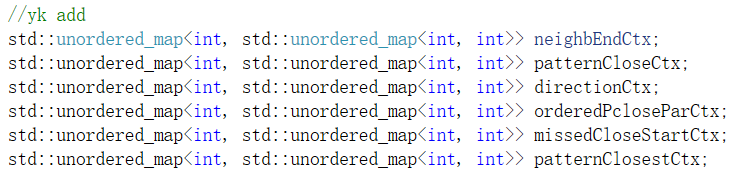
\includegraphics[scale=0.4]{image/键值对.png}
    \caption{键值对代码截图}
    \label{fig:键值对}
\end{figure}

例如计算标识信息时用到的键值对:$std::unordered_map<int, std::unordered_map<int, int>> directionCtx$存储了$direction$的3个不同取值0,1,2与当前待编码边是否被占据的0,1信息匹配的所有情况各自的次数,利用该键值对存储的数据,可以得到$direction=0$时,当前待编码边占据时的占比$rate1$与不占据时的占比$rate0$,同时也可以得到$direction=0$在该类上下文中的占比$countRate$。基于这些数据,利用如下信息熵求解公式\ref{fig:信息熵求解}:
\begin{equation}
    entropy = rate0*\log \frac{1}{{rate0}} + rate1*\log \frac{1}{{rate1}}
    \label{fig:信息熵求解}
\end{equation}
可以得出该类上下文在direction=0时,它的信息熵如公式\ref{fig:信息熵2}所示。
\begin{equation}
    entropy0 = entropy*countRate
    \label{fig:信息熵2}
\end{equation}

同理,$direction=1$和$direction=2$时,可以求出其对应的信息熵$entropy1$,$entropy2$.由此便得到了direction这类上下文的信息熵$entropy=entropy0+entropy1+entropy2$。重复这一计算过程,可以求得编码顶点标识信息
时用到的各类上下文的信息熵。对于其他序列其他码率点的测试,本文采取的方法是:

1、将上述计算方法写入TMC13v20的参考代码,并且在参考代码中加入打印每个slice求得的信息熵的代码后生成可执行文件。

2、撰写python脚本文件将可执行文件用于通测最终测试性能所需的所有点云序列的所有码率点,并将得到的数据结构用txt文本输出。

3、撰写python脚本对所有生成的txt文本进行遍历,获取其中的信息熵并按不同序列的不同码率点输出到excel表格中。其中对于同一码率点的不同slice,将不同slice得到的信息熵进行简单平均作为该码率点的信息熵。

4、重复上述步骤,得到所有测试点云序列的全部码率点下的各类上下文信息熵。

5、最后进行折线图绘制,并分析结果。

以标识信息为例,从四类测试点云序列(solid,dense,sparse,scant)中各取一个测试序列作图,得到其次要信息所用到的上下文的信息熵对比图如\ref{fig:信息熵对比图}所示。

\begin{figure}[h]
    %是可选项 h表示的是here在这里插入,t表示的是在页面的顶部插入
    \centering
    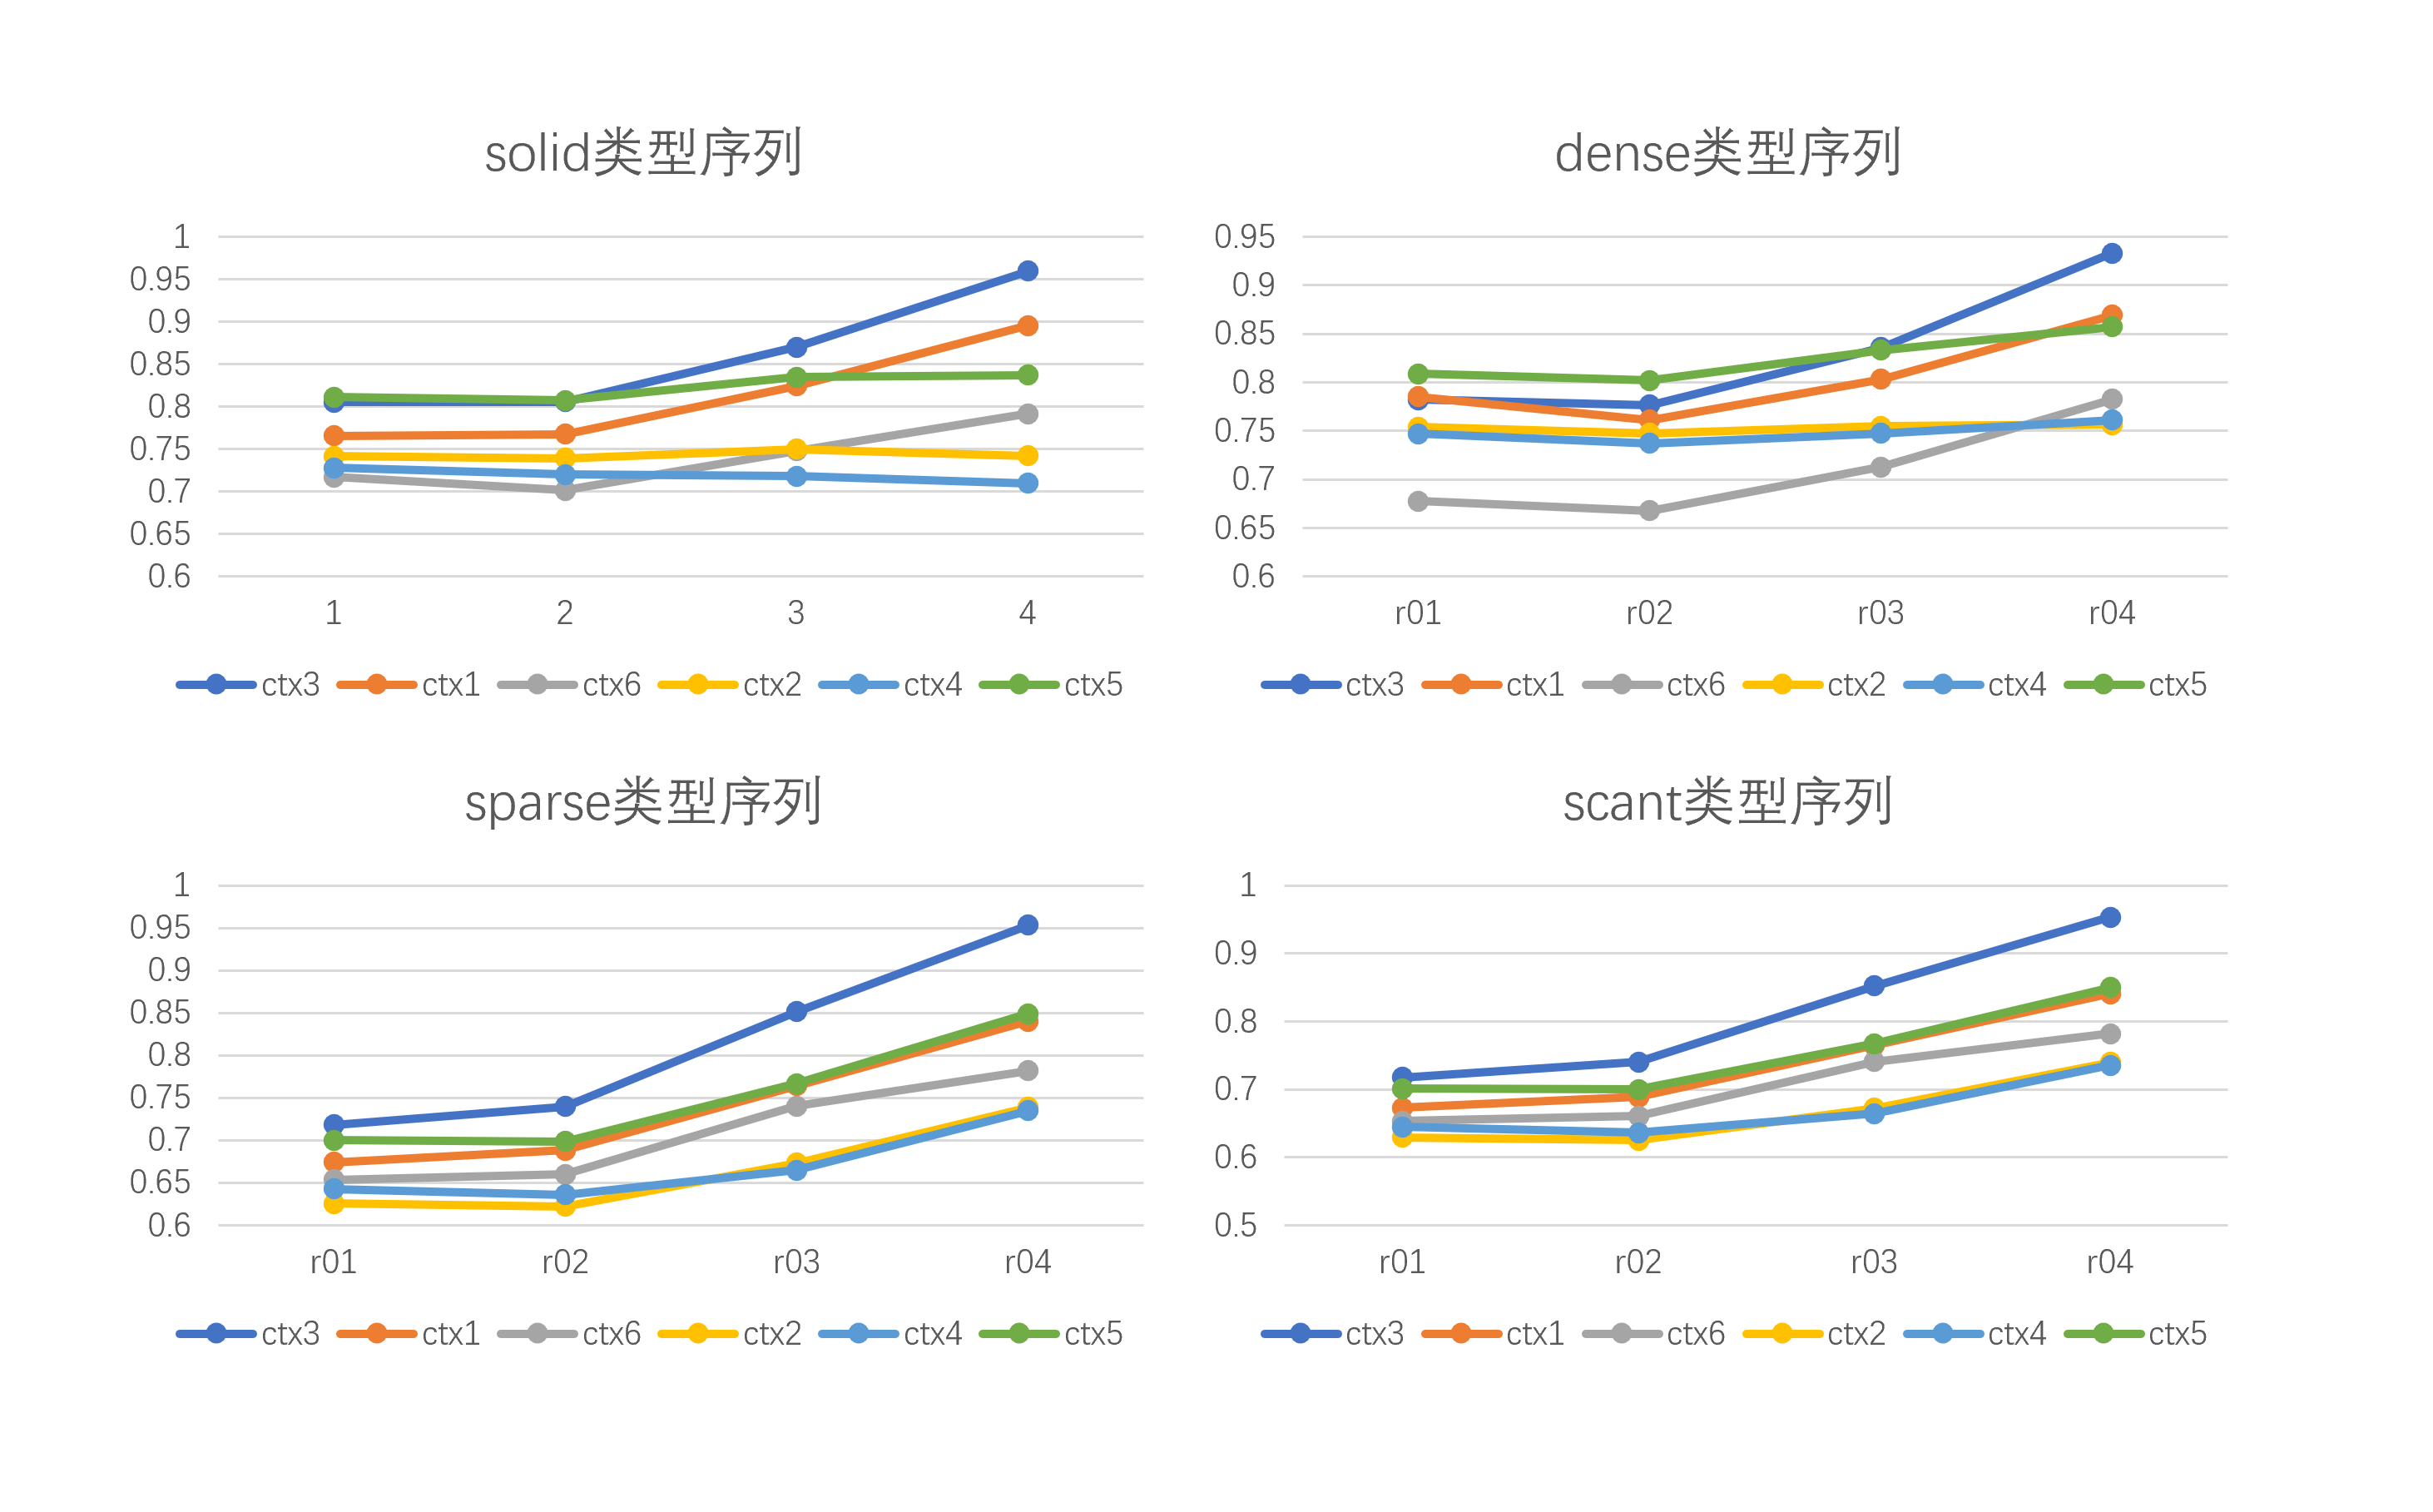
\includegraphics[scale=0.4]{image/flag信息熵对比图.png}
    \caption{标识信息的信息熵对比图}
    \label{fig:信息熵对比图}
\end{figure}

图中我们可以看出在各类点云序列下,ctx4这一上下文基本处于最低熵值的位置,故选取ctx4,即patternClose\&(0b00011000)作为编码顶点标识信息所用到的次要信息的第一个上下文。

同理,对编码顶点位置信息用到的次要信息所包含的上下文信息熵进行测试,可得到如图\ref{fig:位置信息上下文的信息对比图}所示结果。据此得出高bit位应选取ctx4,即patternClose\&(0b00011111)作为其第一类上下文;低bit位应选取ctx5,即patternClose\& (0b00011111)作为其第一类上下文。
\begin{figure}[h]
    %是可选项 h表示的是here在这里插入,t表示的是在页面的顶部插入
    \centering
    \subfloat[高bit位]{
        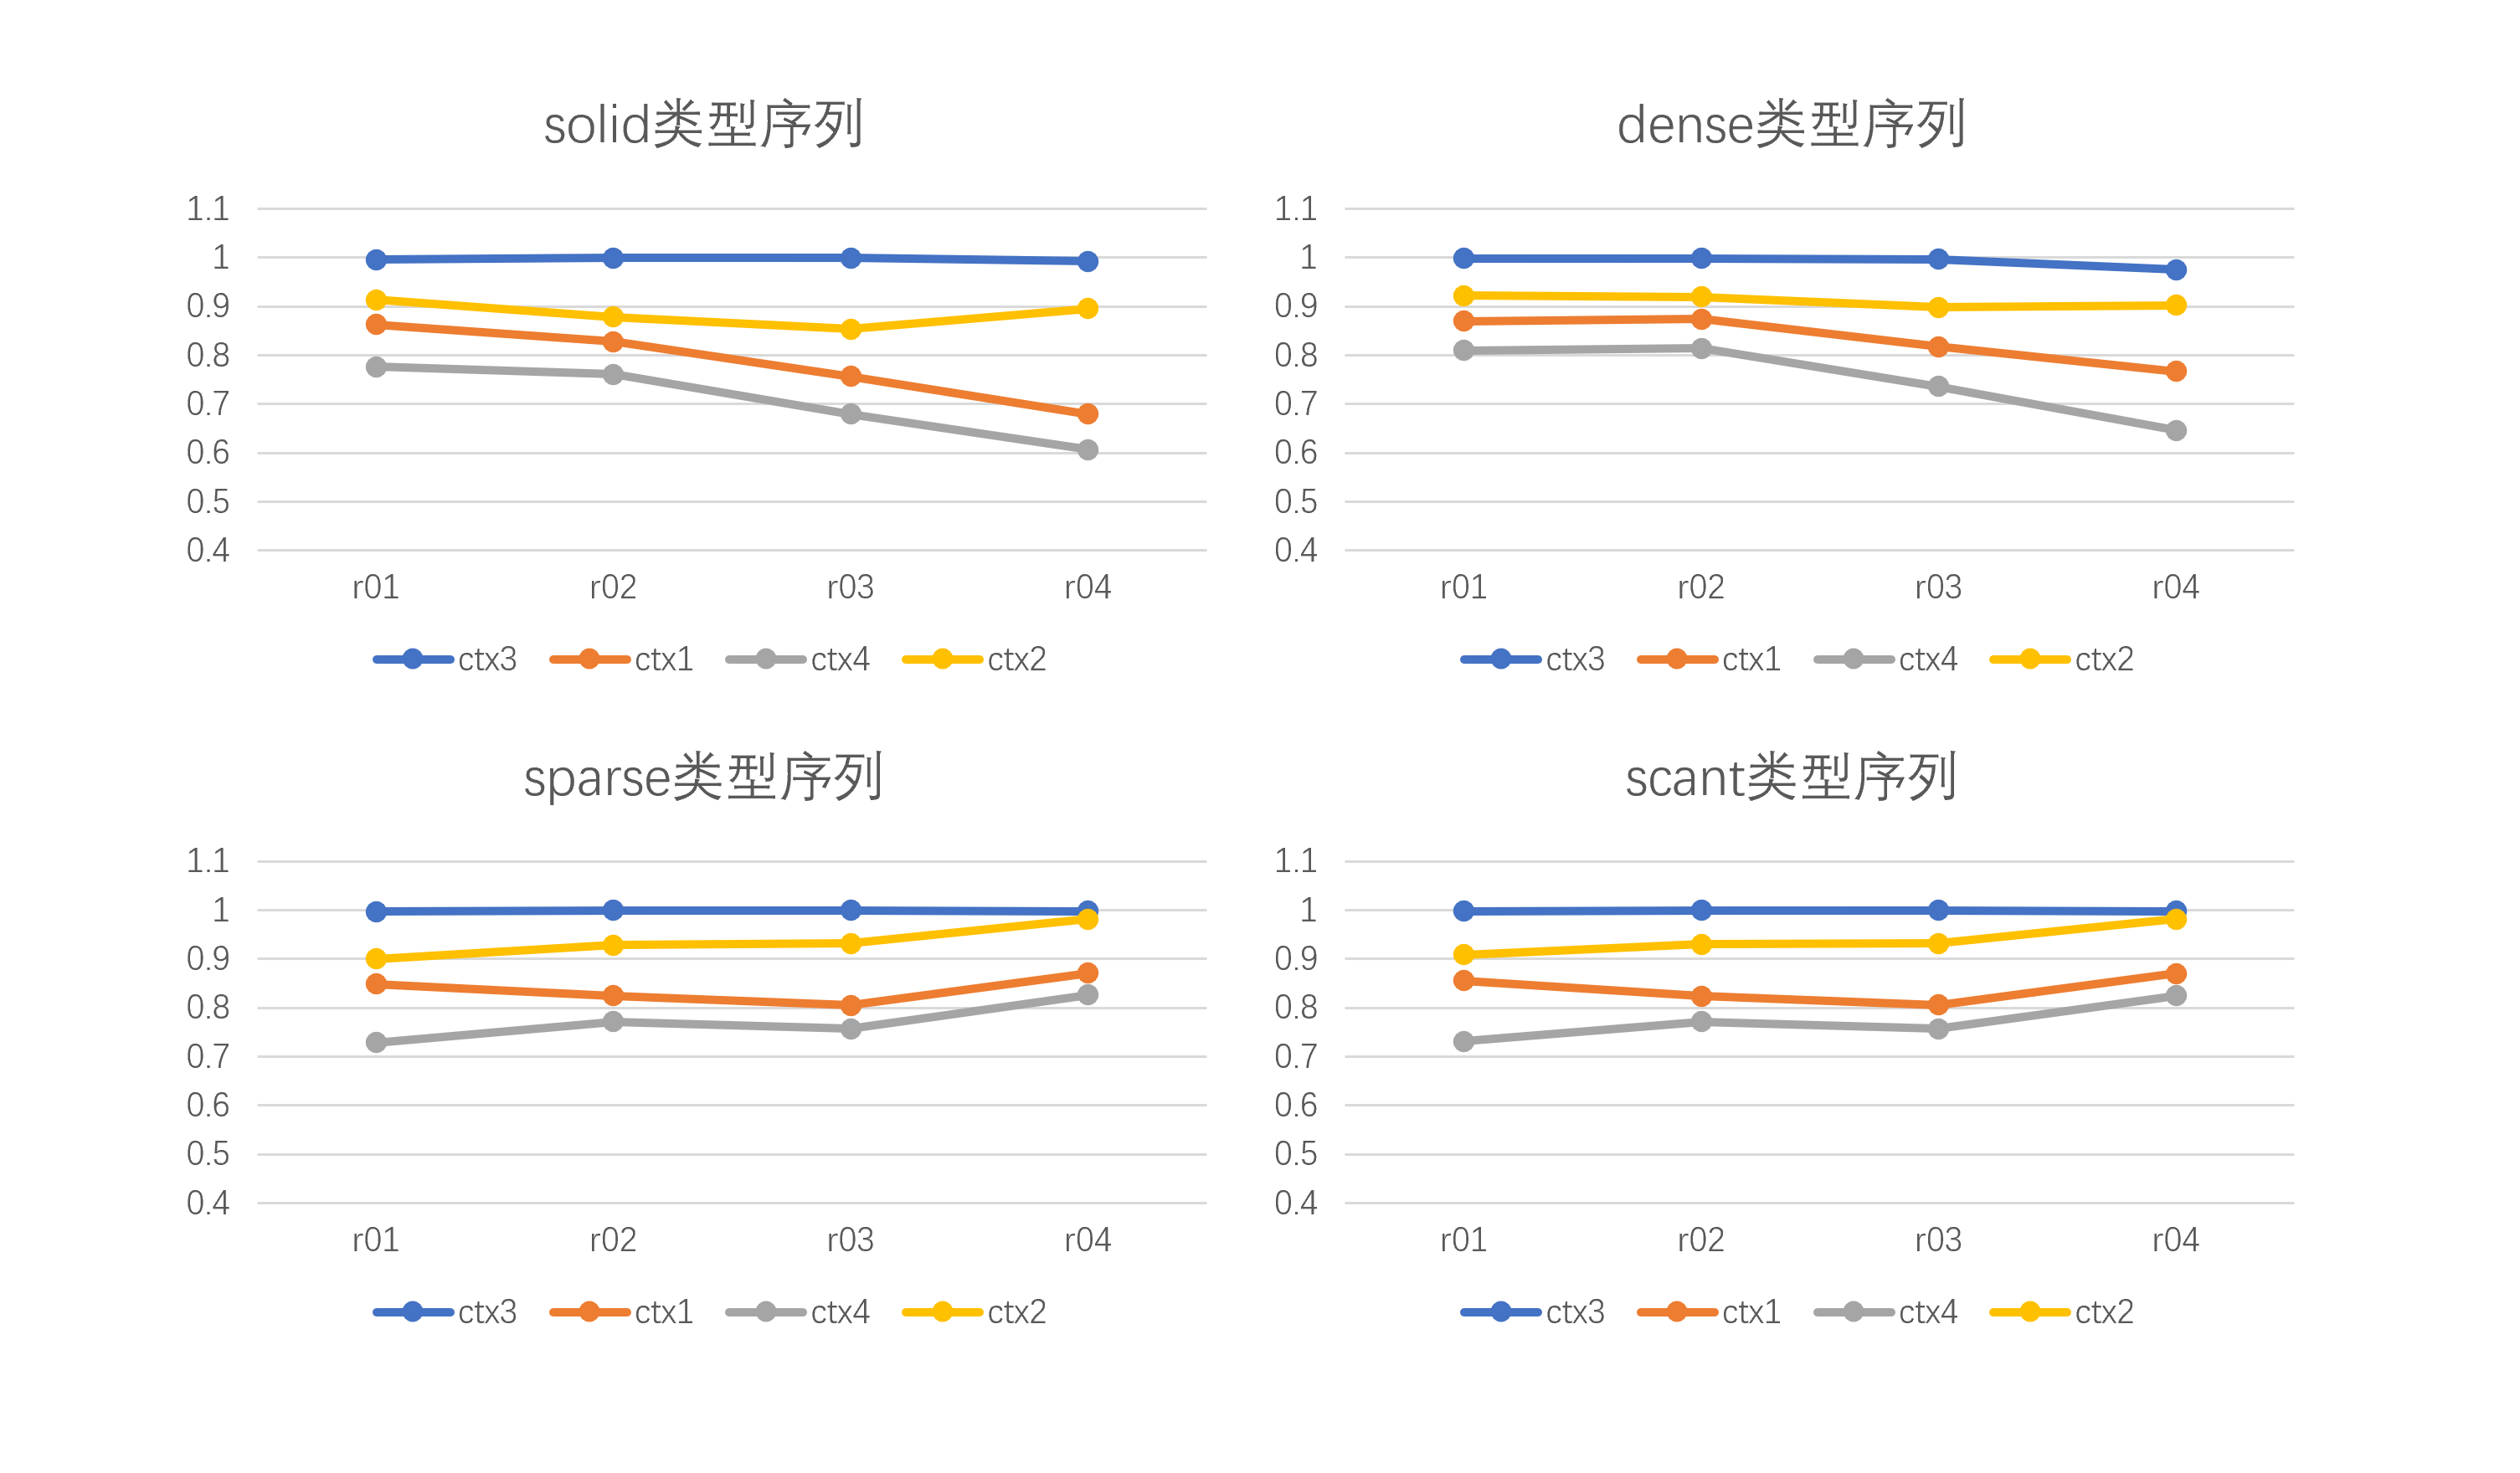
\includegraphics[scale=0.4]{image/高bit位置信息的信息熵.png}
    }
    \hspace{0.1in}
    \subfloat[低bit位]{
        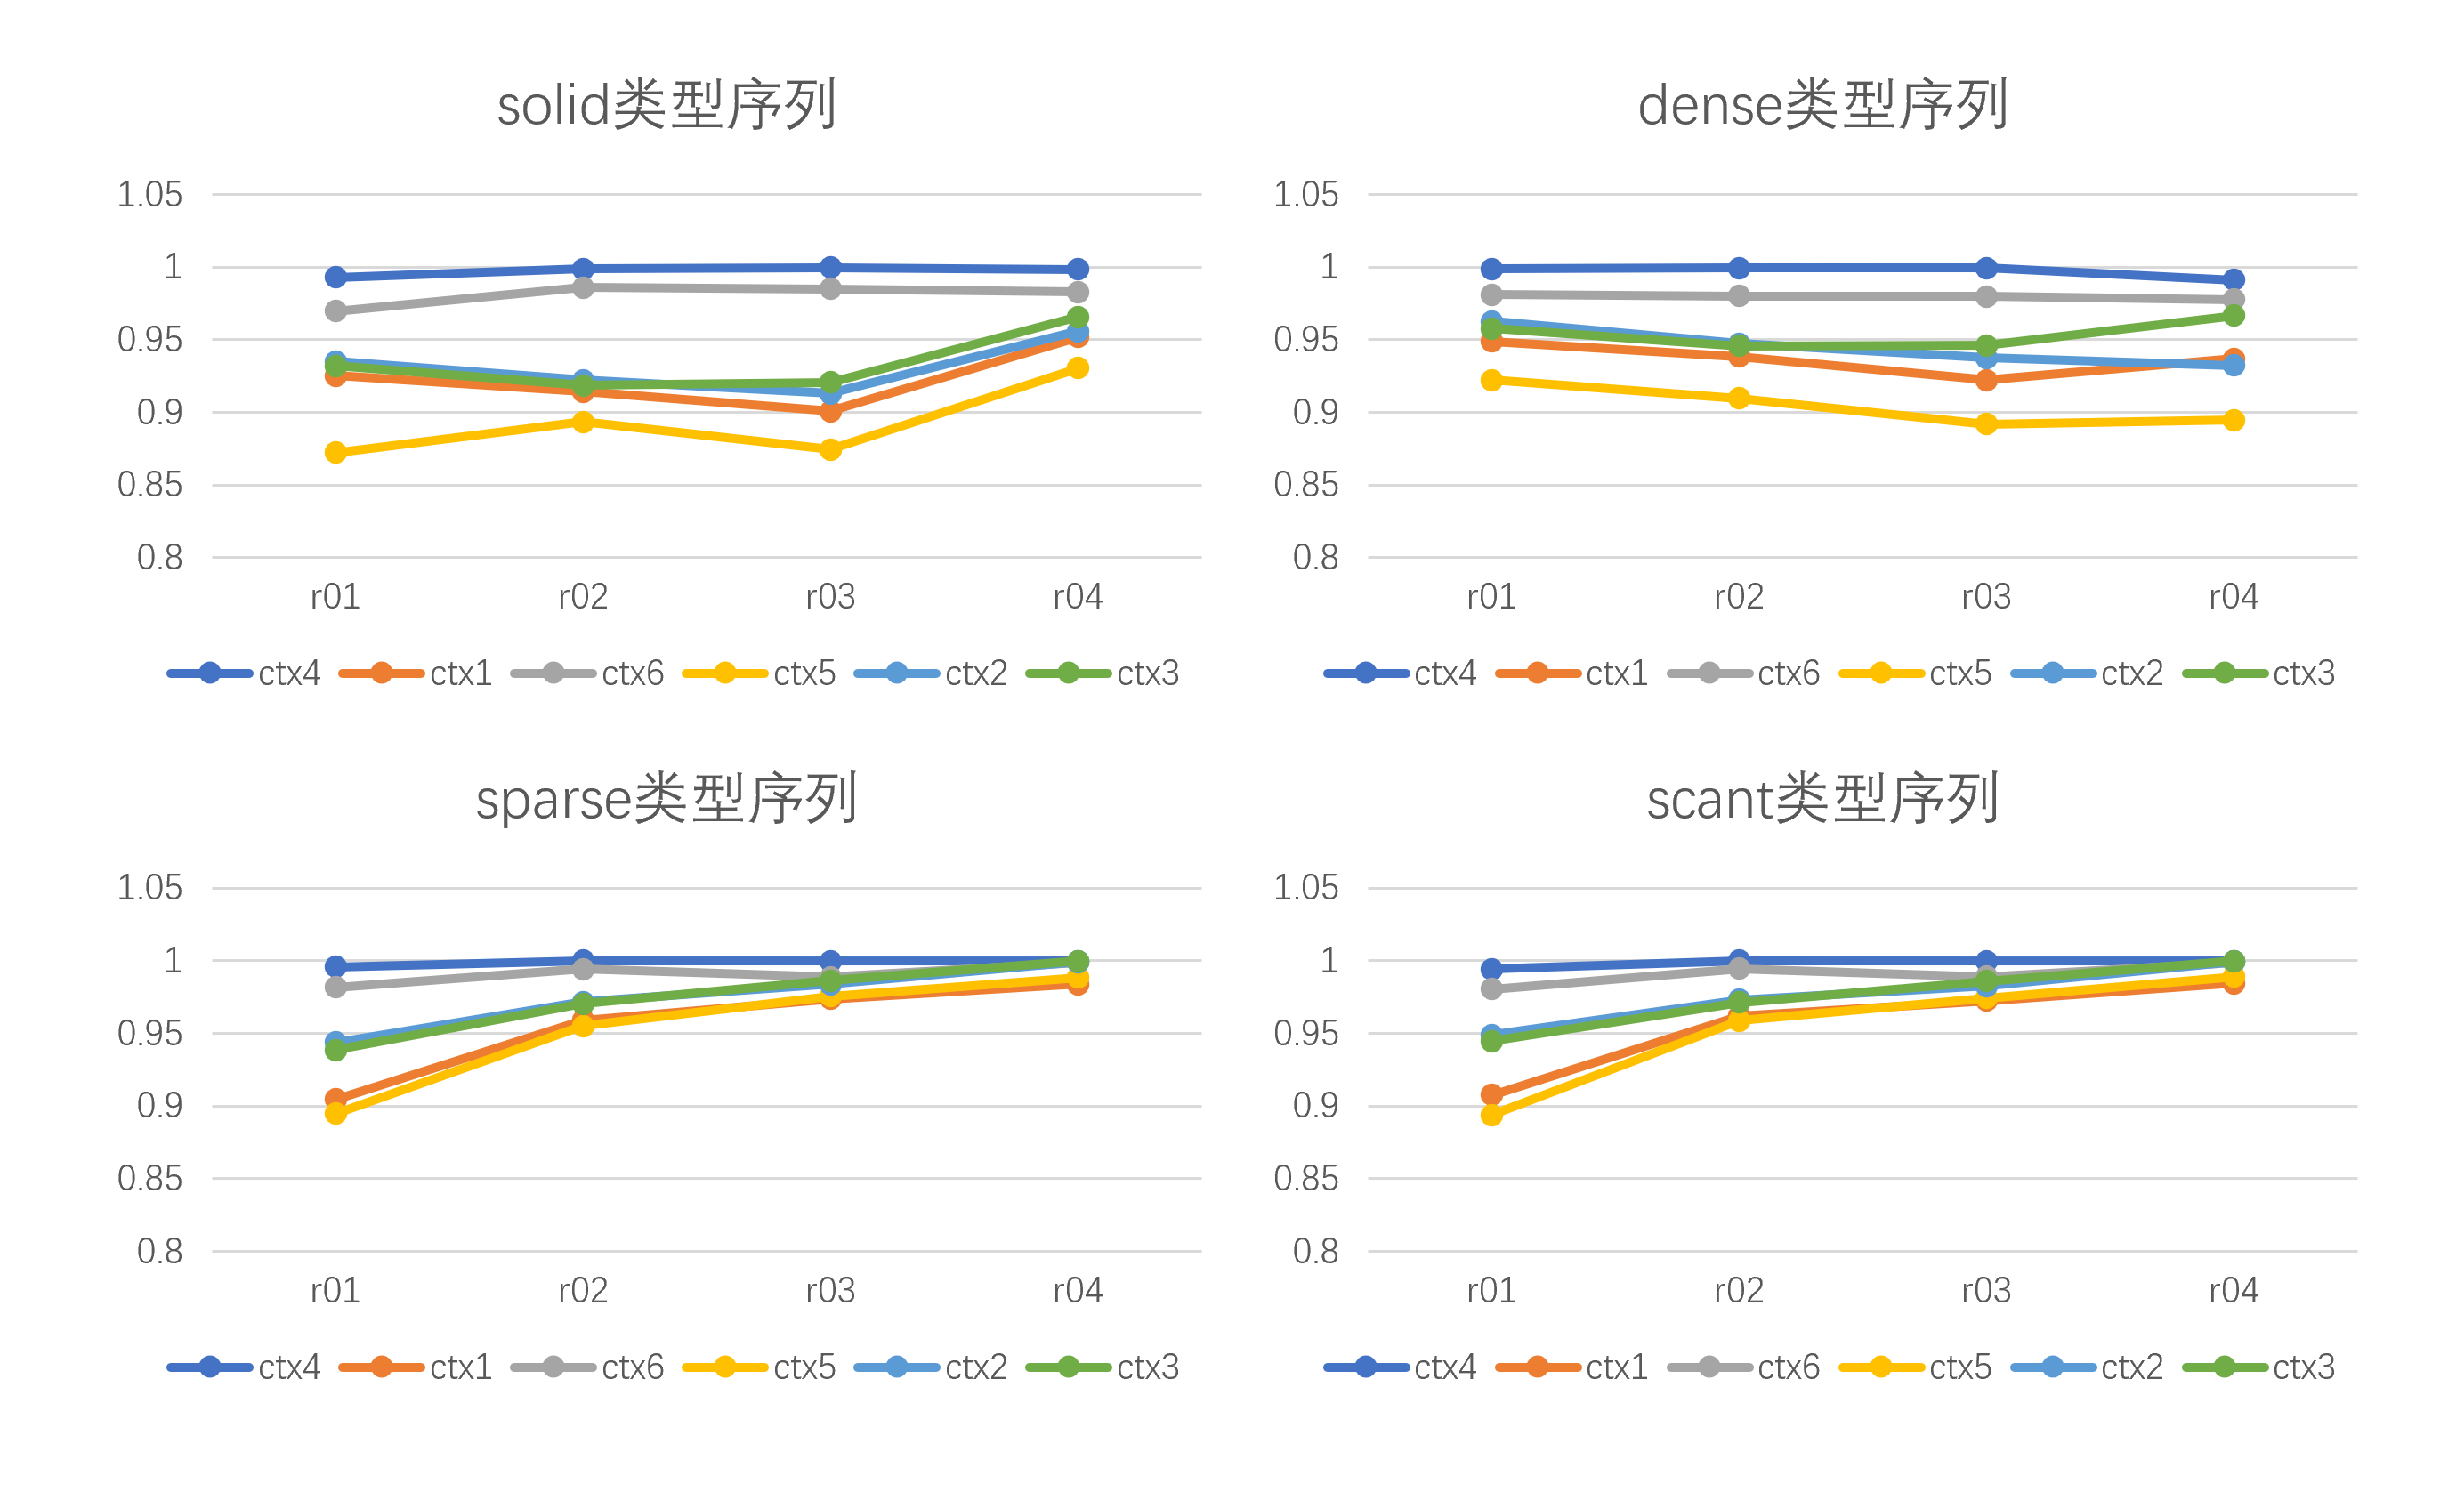
\includegraphics[scale=0.4]{image/低bit位置信息的信息熵.png}
    }
    \caption{位置信息的信息熵对比图}
    \label{fig:位置信息上下文的信息对比图}
\end{figure}
\section{上下文条件熵测量}
基于熵越小,上下文与当前待编码边相关性越强的理论基础,本文在三套上下文的第一类上下文已经确定的基础上对剩余上下文的条件熵进行测试,进而得到三套上下文模型的局部最优顺序。本文条件熵的测试将在$basketball\_player\_vox11\_00000200$序列的$r01$码率点下进行。

以标识信息的上下文条件熵测量为例。依据信息熵的测量结果将$ctx4$作为首要条件,在此条件下对剩余上下文进行条件熵的测试。实际操作过程中,先将$ctx4$分别与剩余五类上下文进行组合构成五类新的上下文,如图\ref{上下文新组合}所示。

\begin{figure}[h]
    %是可选项 h表示的是here在这里插入,t表示的是在页面的顶部插入
    \centering
    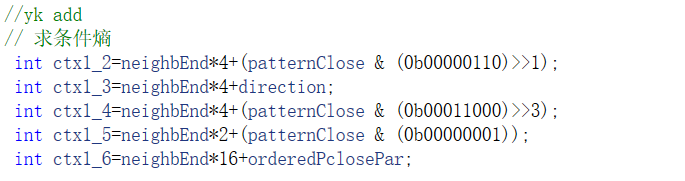
\includegraphics[scale=0.4]{image/上下文新组合.png}
    \caption{组合测试所需上下文部分代码截图}
    \label{上下文新组合}
\end{figure}

从而将对条件熵的测量转换为了对这新的五类熵下文进行信息熵的测量,目的是可以继续使用\ref{上下文信息熵测量}节所介绍的方法。如图\ref{标识信息条件熵}所示,具体实验过程如下:
\begin{figure}[h]
    %是可选项 h表示的是here在这里插入,t表示的是在页面的顶部插入
    \centering
    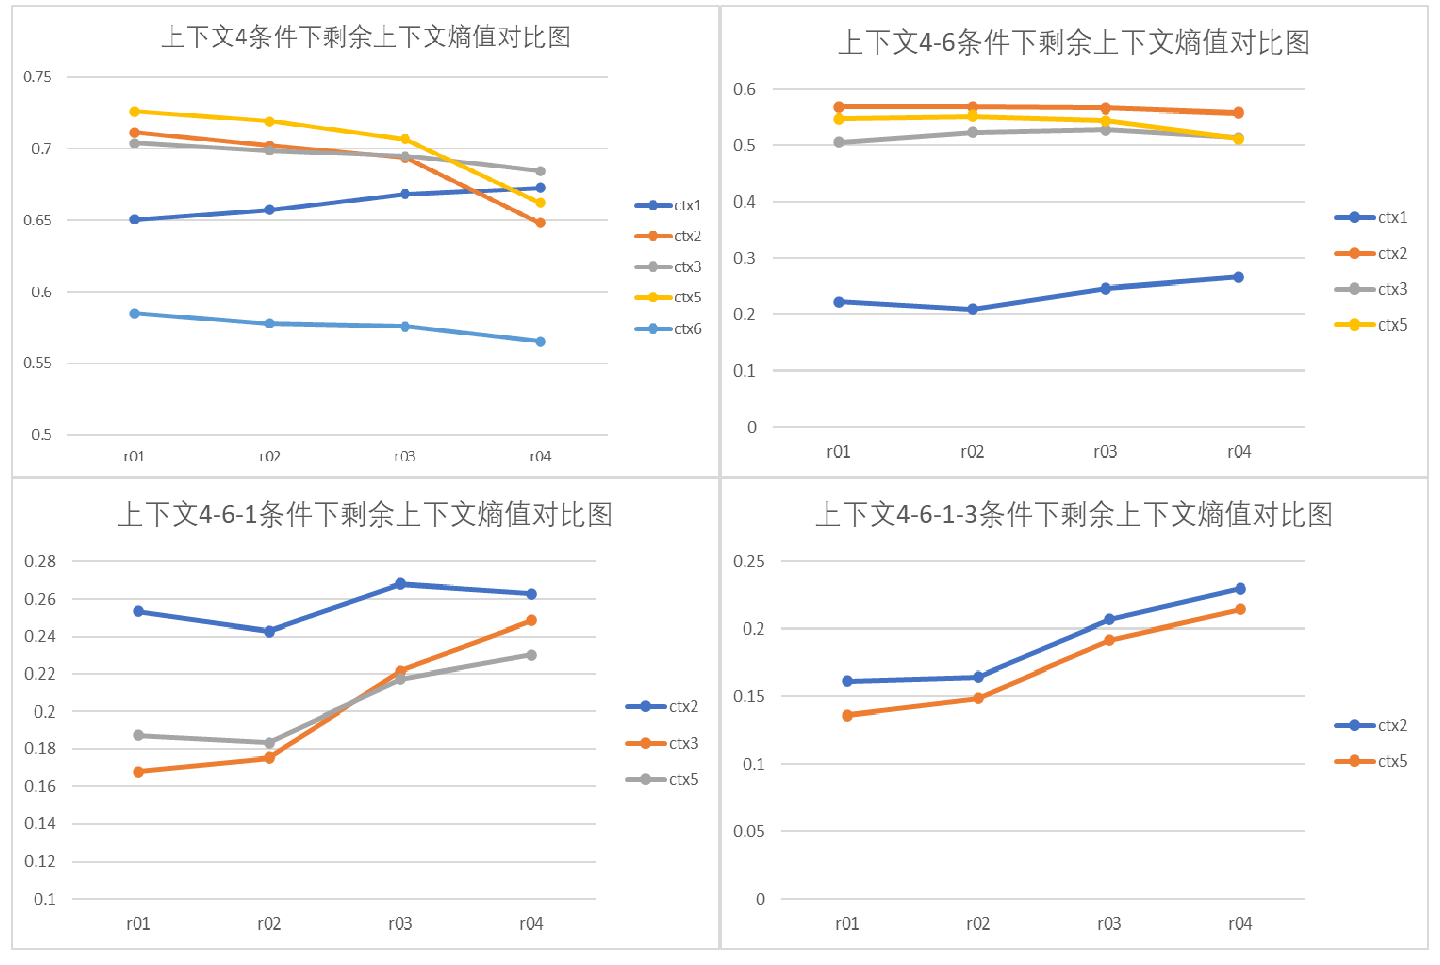
\includegraphics[scale=0.5]{image/标识信息条件熵.pdf}
    \caption{标识信息条件熵对比图}
    \label{标识信息条件熵}
\end{figure}

1、以ctx4作为条件时,测试得到剩余五类上下文的条件熵,得到ctx6条件熵在四个码率点下均明显小于其他四类上下文条件熵,因此选择ctx6作为第二个条件。

2、以ctx4、ctx6作为条件时,测试得到剩余四类上下文的条件熵,得到ctx1条件熵在四个码率点下明显小于其他三类上下文条件熵,因此选择ctx1作为第三个条件。

3、以ctx4、ctx6、ctx1作为条件时,测试得到剩余三类上下文的条件熵。此时得到ctx3在r01与r02码率点下条件熵低于ctx5,但是在r03与r04码率点下,ctx3的条件熵比ctx5的条件熵高。对于这种情况,将四个码率点的条件熵取平均,然后比较其大小。最终得出ctx3在此条件下四个码率点的平均条件熵要小于ctx5,因此选择cxt3作为第四个条件。

4、至此,仅剩下ctx2与ctx5未进行测试,在先前四类上下文的条件下,测量其条件熵,得到ctx5条件在四个码率点小均明显小于ctx2条件熵,因此ctx5将在ctx2前作为上下文被使用。

最终得到编码顶点标识信息时,其次要信息所包含的上下文的顺序应为ctx4-ctx6-ctx1-ctx3-ctx5-ctx2。

对于2bit位置信息,它们条件熵的具体测试过程与标识信息一致,在此不再赘述,给出其测试过程的条件熵对比图如\ref{位置信息条件熵对比图}所示。

\begin{figure}[h]
    %是可选项 h表示的是here在这里插入,t表示的是在页面的顶部插入
    \centering
    \subfloat[高bit位置信息条件熵对比图]{
        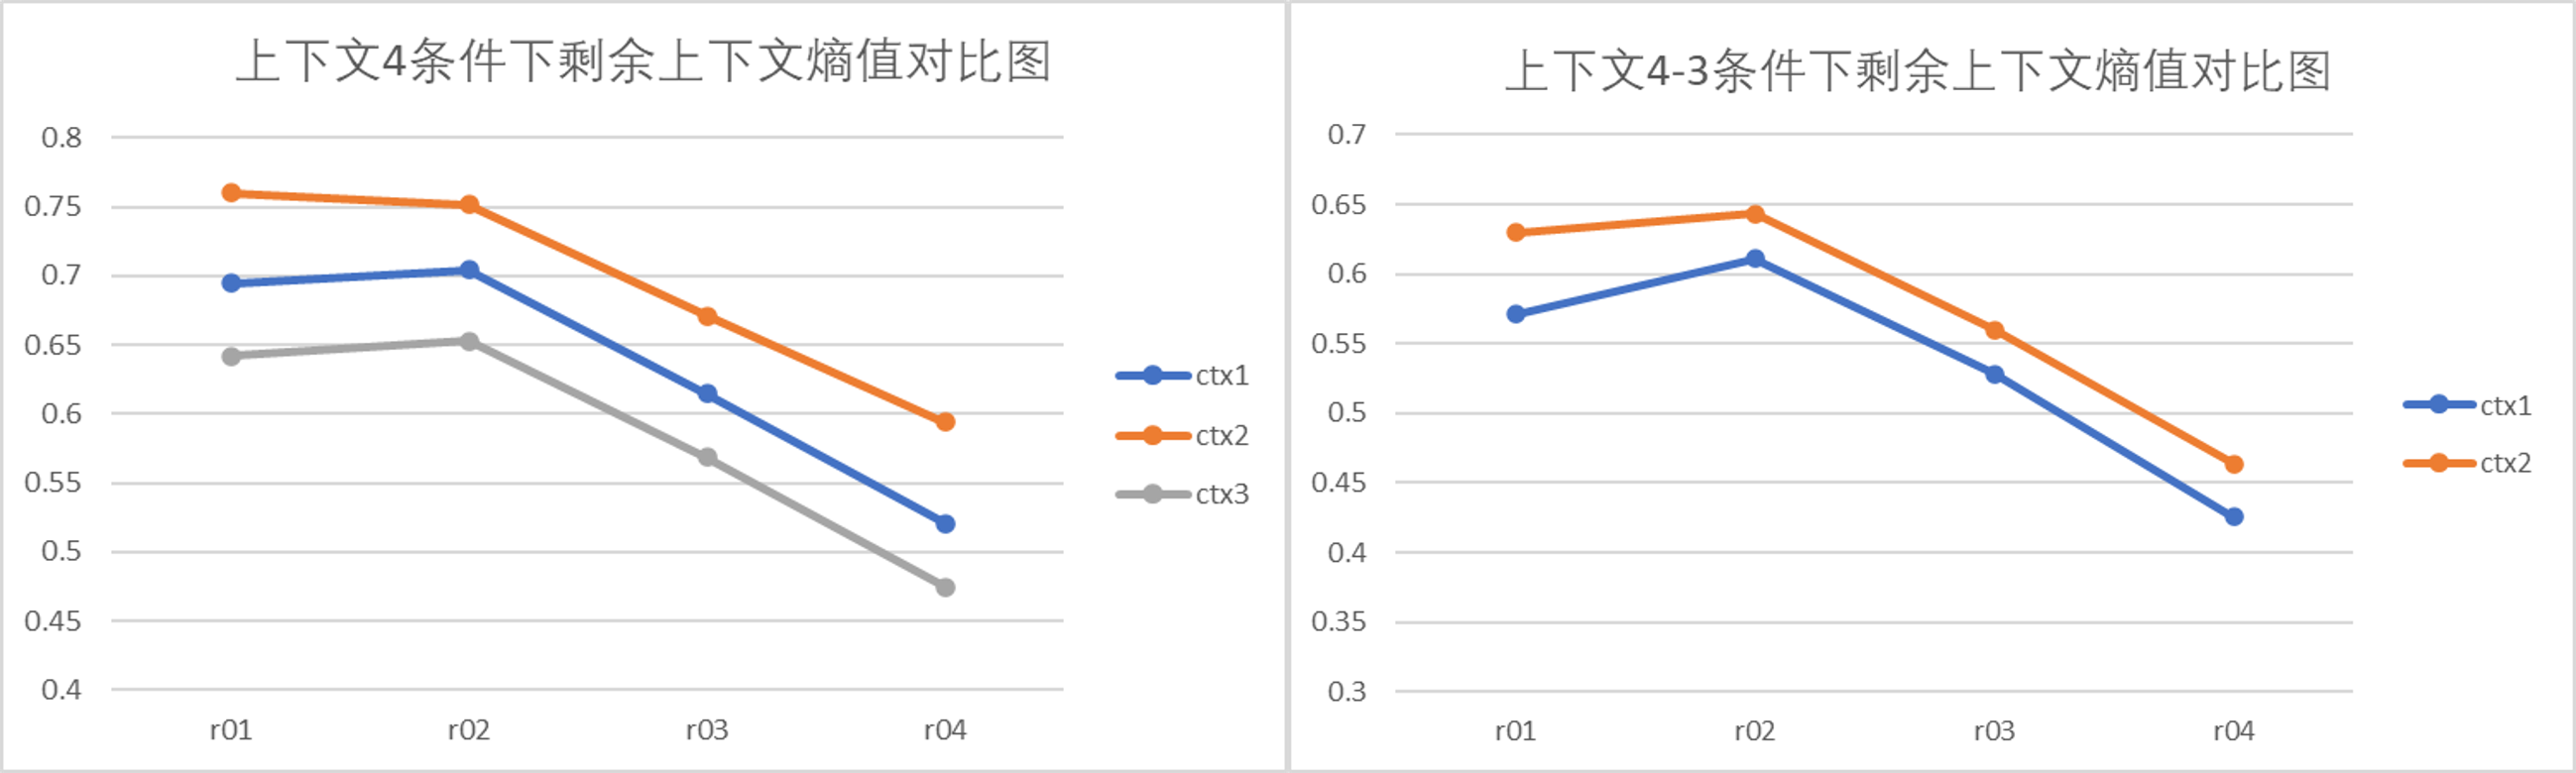
\includegraphics[scale=0.5]{image/高bit位置信息条件熵对比图.png}
    }

    \subfloat[低bit位置信息条件熵对比图]{
        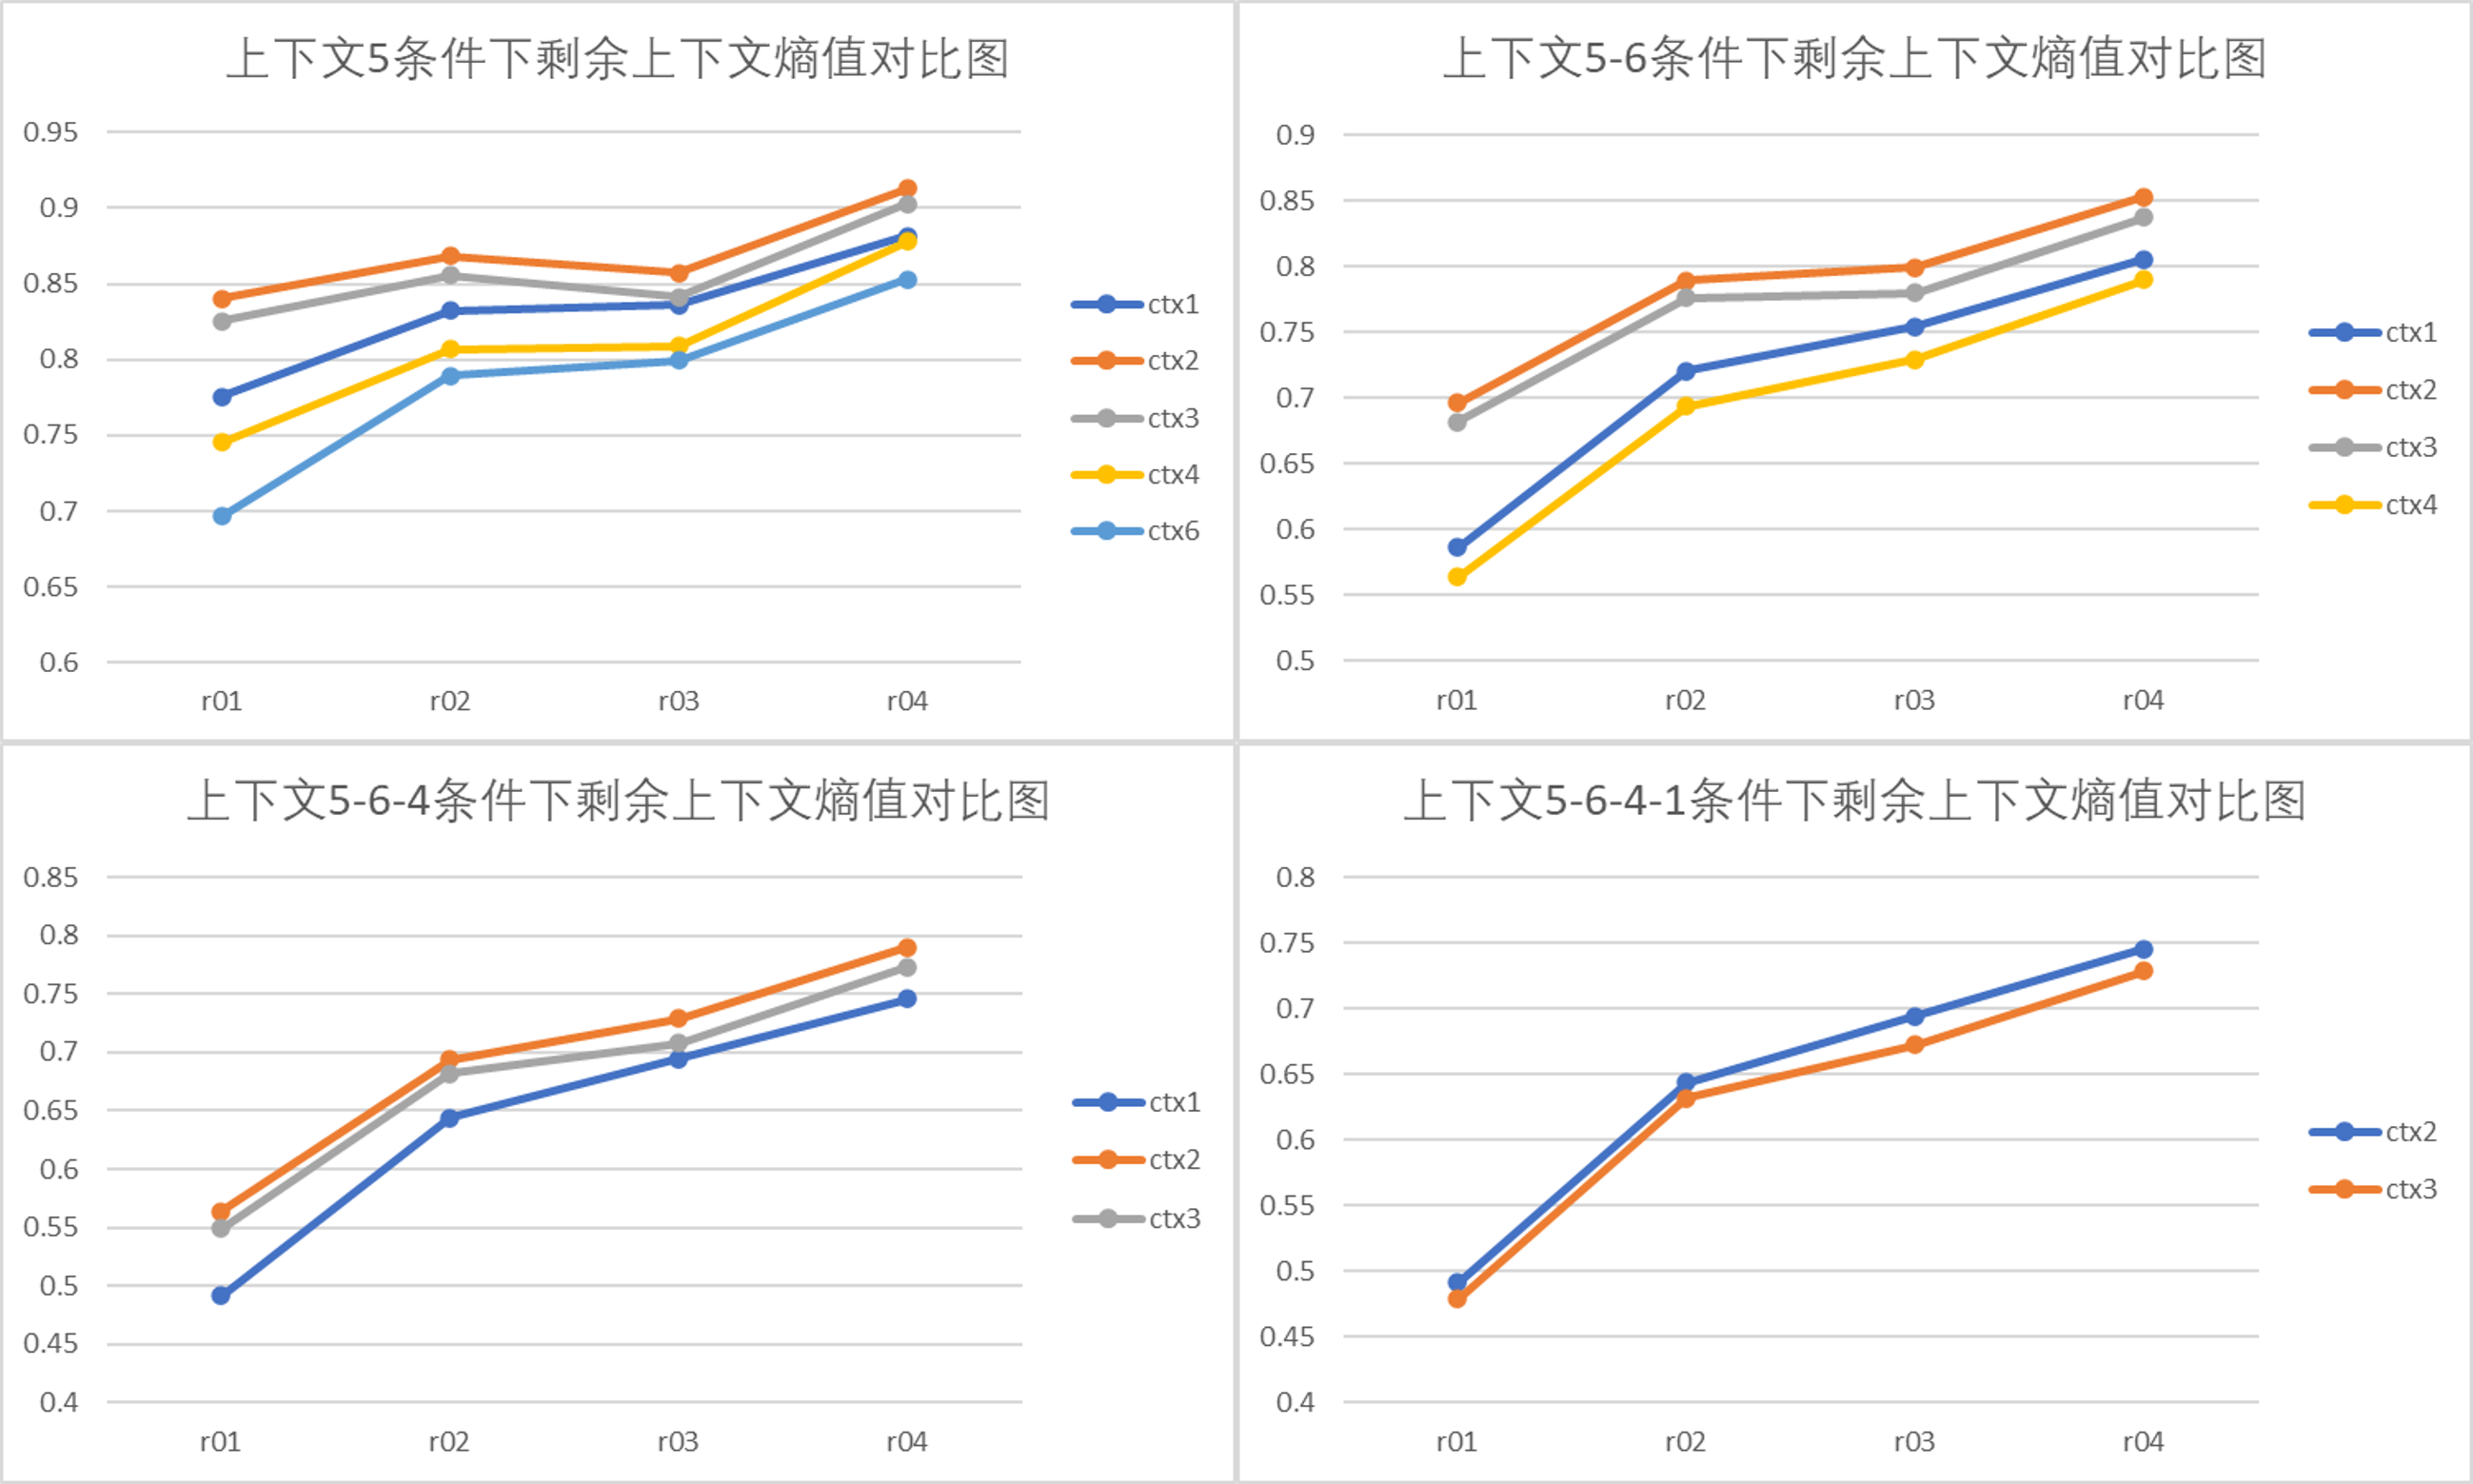
\includegraphics[scale=0.5]{image/低bit位置信息条件熵对比图.png}
    }
    \caption{位置信息条件熵对比图}
    \label{位置信息条件熵对比图}
\end{figure}

由图可以得出,对于编码高bit位置信息时,它所用到的次要信息所包含的上下文的顺序为ctx4-ctx3-ctx1-ctx2;对于编码低bit位置信息时,他所用用到的次要信息所包含的上下文的顺序为ctx5-ctx6-ctx4-ctx1-ctx3-ctx2。
\section{本章小结}
本章首先介绍了Trisoup几何信息编码算法在利用基于OBUF的熵编码时所采用的上下文模型,同时分析了现有上下文模型可能存在的改进空间,然后通过计算并对比各个上下文模型的信息熵与条件熵的大小,得到了一套全新的局部最优的上下文模型。
% \DeclareOption{secret}{\xdu@secrettrue}
% \DeclareOption{english}{\xdu@englishtrue}
% \DeclareOption{print}{\xdu@printtrue}
% \DeclareOption{msfonts}{\xdu@msfontstrue}
% \DeclareOption{adobefonts}{\xdu@msfontsfalse}

\ifx\allfiles\undefined
\end{document}
\fi
%% ----------------------------------------------------------------------
%%% END OF FILE 
%% ----------------------------------------------------------------------
%% ----------------------------------------------------------------------
%% START OF FILE
%% ----------------------------------------------------------------------
%% 
%% Filename: ch03-frontmatter.tex
%% Author: Fred Qi
%% Created: 2012-12-26 09:12:47(+0800)
%% 
%% ----------------------------------------------------------------------
%%% CHANGE LOG
%% ----------------------------------------------------------------------
%% Last-Updated: 2016-02-08 16:55:23(-0700) [by Fred Qi]
%%     Update #: 53
%% ----------------------------------------------------------------------
\ifx\allfiles\undefined
\documentclass[bachelor,print,msfonts]{xduthesis}

% 这里是可能用到的其他宏包,根据自己论文撰写的需要添加
\usepackage{listings}
\usepackage{overpic}
\lstset{language=TeX, basicstyle=\ttfamily}


\newcommand{\figref}[1]{图\ref{#1}}
\newcommand{\sArt}{state-of-the-art}
\newcommand{\wyh}[1]{{\textcolor{blue}{#1}}}
\newcommand{\secref}[1]{Sec. \ref{#1}}
\newcommand{\tabref}[1]{Tab.~\ref{#1}}
\newcommand{\thudot}[1]{} % thubib.bst 定义每条参考文献最后的点\thudot
\graphicspath{{./}{./img/}{./fig/}{./image/}{./figure/}{./picture/}}
\newcommand{\bs}{\boldsymbol}
\usepackage{float}
\usepackage{longtable}
\usepackage{tcolorbox}
\setcounter{chapter}{2}
\begin{document}
\mainmatter
\fi

\chapter{实验条件与结果分析}
\label{cha:frontmatter}
MPEG针对第一类静态点云序列和第三类动态点云序列构建了TMC13测试平台。并且针对不同版本的测试平台,发布了Common test conditions for GPCC\cite{ref23}的文件来统一测试条件。本次实验的参考测试平台是TMC13v20.0,实验使用的测试条件、软件配置情况与TMC13v20.0的通用测试条件、软件参考配置保持一致。测试得到的性能结果也是相对于TMC13v20.0性能的增益情况。
\section{实验配置}
\subsection{测试序列}
本次实验测试的序列是根据点云的稠密程度划分的四类静态点云序列:具有连续表面的体素化点云(solid)、表面不完全连续的体素化点云(dense)、稀疏点云(sparse)、极其稀疏点云(scant)。下表 \ref{tab3} 介绍了四类点云序列中各种序列的参数情况。点数表示每个点云序列包含的所有点的个数,几何精度指示每个点云序列的几何信息表示精度,帧数表示每个点云序列包含点云帧的个数,本次实验测试的都是单帧点云,所以帧数都为1。属性格式指示的是点云属性的类型,有颜色 RGB 和反射率 reflectance 两种类型。

{
\tiny
\begin{longtable}{cccccc}
    %\fontsize{10.5pt}{15pt}\selectfont
    %\centering
    \caption{点云测试序列参数列表}
    \label{tab3}                                                                                              \\
    %\begin{tabular}{cccccc}
    \toprule
    序列种类              & 序列名                              & 点数     & 几何精度/bit位 & 帧数 & 属性格式 \\
    \midrule
    \endfirsthead
    \toprule
    序列种类              & 序列名                              & 点数     & 几何精度/bit位 & 帧数 & 属性格式 \\
    \midrule
    \endhead
    \bottomrule
    \endfoot
    \bottomrule
    \endlastfoot
    \multirow{9}*{solid}  & basketball\_player\_vox11\_00000200 & 2925514  & 11             & 1    & RGB      \\
                          & dancer\_vox11\_00000001             & 2592758  & 11             & 1    & RGB      \\
                          & facade\_00064\_vox11                & 4061755  & 11             & 1    & RGB      \\
                          & longdress\_vox10\_1300              & 857966   & 10             & 1    & RGB      \\
                          & loot\_vox10\_1200                   & 805285   & 10             & 1    & RGB      \\
                          & queen\_0200                         & 1000993  & 10             & 1    & RGB      \\
                          & redandblack\_vox10\_1550            & 757691   & 10             & 1    & RGB      \\
                          & soldier\_vox10\_0690                & 1089091  & 10             & 1    & RGB      \\
                          & thaidancer\_viewdep\_vox12          & 3130215  & 12             & 1    & RGB      \\

    \midrule
    \multirow{12}*{dense} & boxer\_viewdep\_vox12               & 3493085  & 12             & 1    & RGB      \\
                          & facade\_00009\_vox12                & 1596085  & 12             & 1    & RGB      \\
                          & facade\_00015\_vox14                & 8907880  & 14             & 1    & RGB      \\
                          & facade\_00064\_vox14                & 19702134 & 14             & 1    & RGB      \\
                          & frog\_00067\_vox12                  & 3614251  & 12             & 1    & RGB      \\
                          & head\_00039\_vox12                  & 13903516 & 12             & 1    & RGB      \\
                          & house\_without\_roof\_00057\_vox12  & 4848745  & 12             & 1    & RGB      \\
                          & landscape\_00014\_vox14             & 71948094 & 14             & 1    & RGB      \\
                          & longdress\_viewdep\_vox12           & 3096122  & 12             & 1    & RGB      \\
                          & loot\_viewdep\_vox12                & 3017285  & 12             & 1    & RGB      \\
                          & vredandblack\_viewdep\_vox12        & 2770567  & 12             & 1    & RGB      \\
                          & soldier\_viewdep\_vox12             & 4001754  & 12             & 1    & RGB      \\

    \midrule
    \multirow{12}*{dense} & arco\_valentino\_dense\_vox12       & 1481746  & 12             & 1    & RGB      \\
                          & arco\_valentino\_dense\_vox12       & 1481746  & 12             & 1    & RGB      \\
                          & egyptian\_mask\_vox12               & 272684   & 12             & 1    & RGB      \\
                          & palazzo\_carignano\_dense\_vox14    & 4187594  & 14             & 1    & RGB      \\
                          & shiva\_00035\_vox12                 & 1009132  & 12             & 1    & RGB      \\
                          & stanford\_area\_2\_vox16            & 47062002 & 16             & 1    & RGB      \\
                          & stanford\_area\_4\_vox16            & 43399204 & 16             & 1    & RGB      \\
                          & staue\_klimt\_vox12                 & 499660   & 12             & 1    & RGB      \\
                          & ulb\_unicorn\_hires\_vox15          & 63787119 & 15             & 1    & RGB      \\
                          & ulb\_unicorn\_vox13                 & 1995189  & 13             & 1    & RGB      \\

    \midrule
    \multirow{12}*{dense} & arco\_valentino\_dense\_vox20       & 1530552  & 20             & 1    & RGB      \\
                          & egyptian\_mask\_vox20               & 272689   & 20             & 1    & RGB      \\
                          & facade\_00009\_vox20                & 1602990  & 20             & 1    & RGB      \\
                          & facade\_00015\_vox20                & 8929532  & 20             & 1    & RGB      \\
                          & facade\_00064\_vox20                & 19714629 & 20             & 1    & RGB      \\
                          & frog\_00067\_vox20                  & 3630907  & 20             & 1    & RGB      \\
                          & head\_00039\_vox20                  & 14025709 & 20             & 1    & RGB      \\
                          & house\_without\_roof\_00057\_vox20  & 5001077  & 20             & 1    & RGB      \\
                          & landscape\_00014\_vox20             & 72145549 & 20             & 1    & RGB      \\
                          & palazzo\_carignano\_dense\_vox20    & 4203962  & 20             & 1    & RGB      \\
                          & shiva\_00035\_vox20                 & 1010591  & 20             & 1    & RGB      \\
                          & stanford\_area\_2\_vox20            & 47062018 & 20             & 1    & RGB      \\
                          & stanford\_area\_4\_vox20            & 43399207 & 20             & 1    & RGB      \\
                          & staue\_klimt\_vox20                 & 499886   & 20             & 1    & RGB      \\
                          & ulb\_unicorn\_hires\_vox20          & 63864641 & 20             & 1    & RGB      \\
                          & ulb\_unicorn\_vox20                 & 2000297  & 20             & 1    & RGB      \\
    %\end{tabular}
\end{longtable}
}
\subsection{测试条件}

GPCC将通用测试条件根据几何、属性部分是否有损分为4种测试条件:C1(Lossless Geometry – Lossy attributes)代表着几何无损、属性有损;C2(Near-lossless | Lossy Geometry – Lossy Attributes)代表着几何有损、属性有损;CW(Lossless Geometry – Lossless Attributes)代表着几何无损、属性无损;C4(Lossless Geometry – Near-lossless Attributes)代表着几何无损、属性有限度有损。通过更改相应配置文件参数,可以实现不同条件的实验配置。本文对Trisoup几何信息编码的熵编码过程进行优化,测试条件是C2,即几何有损,属性有损。


\section{实验结果分析}
在GPCC中衡量一个编解码器的性能主要从三个方面考虑,一是点云压缩后输出的比特流大小;二是编解码点云的时间复杂度;三是编解码前后点云的失真情况。由于本文仅对trisoup几何信息编码过程中的熵编码过程进行了改动,因此最终的性能结果只需要关注点云压缩后输出的比特流的大小变化与编解码点云的时间复杂度的变化。D1,D2用来衡量本文所提出的改进方案是否带来性能提升,其中,D1用来表示点对点的几何失真,D2用来表示点对面的几何失真。当其值小于零时,表明改进方案存在性能增益,当其值大于零时,表明改进方案相比于现有压缩方案带来了一定loss。之所以可以用这一综合衡量指标代替比特流大小(bpip ratio)来衡量性能变化,是因为本文所提出的改进方案不对几何重建产生任何影响,即不会影响几何失真。因此D1,D2的变化全部来自于比特流大小变化。
\subsection{上下文改进结果}
\label{实验结果}
1、仅将编码顶点标识信息时基于动态OBUF的熵编码所用到的次要信息中的六类上下文顺序改为:ctx4-ctx6-ctx1-ctx3-ctx5-ctx2,然后对所有测试序列进行压缩性能测试,测试结果与TMC13v20的anchor进行对比,得到综合性能表如表\ref{标识信息性能表}所示:
{
\scriptsize
\begin{table}[h]
    \fontsize{10.5pt}{15pt}\selectfont
    \centering
    \caption{\label{标识信息性能表} 仅修改标识信息上下文的性能表}
    \setlength{\tabcolsep}{10mm}{
        \begin{tabular}{ccc}
            \toprule
            \multirow{3}*{C2\_ai } & \multicolumn{2}{c}{lossy geometry,lossy attributes [all intra]}          \\
                                   & \multicolumn{2}{c}{Geom. BD-TotGeomRate [\%]}                            \\
                                   & D1                                                              & D2     \\
            \midrule
            Solid average          & 1.3\%                                                           & 1.3\%  \\
            Dense average          & 0.9\%                                                           & 1.0\%  \\
            Sparse average         & -0.2\%                                                          & -0.1\% \\
            Scant average          & 0.0\%                                                           & 0.1\%  \\
            \midrule
            Overall average        & 0.5\%                                                           & 0.5\%  \\
            \bottomrule
        \end{tabular} }
\end{table}
}
{
\scriptsize
\begin{table}[h]
    \fontsize{10.5pt}{15pt}\selectfont
    \centering
    \caption{\label{高bit位置信息性能表} 仅修改高bit位置信息上下文的性能表}
    \setlength{\tabcolsep}{10mm}{
        \begin{tabular}{ccc}
            \toprule
            \multirow{3}*{C2\_ai } & \multicolumn{2}{c}{lossy geometry,lossy attributes [all intra]}         \\
                                   & \multicolumn{2}{c}{Geom. BD-TotGeomRate [\%]}                           \\
                                   & D1                                                              & D2    \\
            \midrule
            Solid average          & 0.6\%                                                           & 0.6\% \\
            Dense average          & 0.4\%                                                           & 0.5\% \\
            Sparse average         & 0.6\%                                                           & 0.6\% \\
            Scant average          & 0.6\%                                                           & 0.6\% \\
            \midrule
            Overall average        & 0.5\%                                                           & 0.6\% \\
            \bottomrule
        \end{tabular} }
\end{table}
}

2、仅将编码顶点位置信息的高bit位时次要信息上下文顺序改为:ctx4-ctx3-ctx1-ctx2,然后对所有测试序列进行压缩性能测试,测试结果与TMC13v20的anchor进行对比,得到综合性能表如表\ref{高bit位置信息性能表}所示;仅将编码顶点位置信息的低bit位时次要信息上下文顺序改为:ctx5-ctx6-ctx4-ctx1-ctx3-ctx2,然后对所有测试序列进行压缩性能测试,测试结果与TMC13v20的anchor进行对比,得到综合性能表如表\ref{低bit位置信息性能表}所示。

{
\scriptsize
\begin{table}[h]
    \fontsize{10.5pt}{15pt}\selectfont
    \centering
    \caption{\label{低bit位置信息性能表} 仅修改低bit位置信息上下文的性能表}
    \setlength{\tabcolsep}{10mm}{
        \begin{tabular}{ccc}
            \toprule
            \multirow{3}*{C2\_ai } & \multicolumn{2}{c}{lossy geometry,lossy attributes [all intra]}         \\
                                   & \multicolumn{2}{c}{Geom. BD-TotGeomRate [\%]}                           \\
                                   & D1                                                              & D2    \\
            \midrule
            Solid average          & 0.4\%                                                           & 0.4\% \\
            Dense average          & 0.2\%                                                           & 0.2\% \\
            Sparse average         & 0.6\%                                                           & 0.7\% \\
            Scant average          & 0.5\%                                                           & 0.5\% \\
            \midrule
            Overall average        & 0.4\%                                                           & 0.4\% \\
            \bottomrule
        \end{tabular} }
\end{table}
}

{
\scriptsize
\begin{table}[h]
    \fontsize{10.5pt}{15pt}\selectfont
    \centering
    \caption{\label{整体修改性能表} 整体修改性能表}
    \setlength{\tabcolsep}{10mm}{
        \begin{tabular}{ccc}
            \toprule
            \multirow{3}*{C2\_ai } & \multicolumn{2}{c}{lossy geometry,lossy attributes [all intra]}         \\
                                   & \multicolumn{2}{c}{Geom. BD-TotGeomRate [\%]}                           \\
                                   & D1                                                              & D2    \\
            \midrule
            Solid average          & 2.1\%                                                           & 2.1\% \\
            Dense average          & 1.2\%                                                           & 1.3\% \\
            Sparse average         & 0.2\%                                                           & 0.2\% \\
            Scant average          & 0.3\%                                                           & 0.3\% \\
            \midrule
            Overall average        & 0.9\%                                                           & 0.9\% \\
            \bottomrule
        \end{tabular} }
\end{table}
}

3、将编码顶点标识信息和位置信息的上下文均按照条件熵递增的顺序修改后,我们得到本此研究实验的最终性能表如表\ref{整体修改性能表}所示。

\subsection{结果分析}
从\ref{实验结果}小节所展示的性能表可以看出,除了在修改标识信息上下文时,在sparse类型序列上整体有0.2\%的增益外,不论是单独看修改每部分上下文后的性能表还是看将三套上下文模型均修改后的性能表,得到的均是负增益。但是在C2测试条件下,展开查看各个序列的性能结果后发现,有个别序列性能增益较大,如表\ref{有增益序列}所示。

由于同样也存在较多的负增益很大的序列,所以导致整体性能呈现负增益。本文在最初分析如何进行上下文改进时有提到,通过求解现有上下文的信息熵然后再基于信息熵最小的上下文一层一层按照条件熵递增的顺序排列剩余上下文的方法,得到的只能是局部的最优解,因为无法确定当选取信息熵较大的序列为第一个上下文后,其他上下文在此条件下会不会有更优异的性能,从而致使整体性能优于本文所得到的上下文顺序。为此,本文进行了一项额外实验,假设现有上下文顺序是通过一定方法选择出来的较优顺序,那么不改变现有上下文模型中排在最前面的那类上下文的位置,而剩余上下文仍旧按照条件熵递增的顺序排列,得到如图\ref{额外实验性能表}所示性能表。
\begin{table}[h]
    \fontsize{10.5pt}{15pt}\selectfont
    \centering
    \caption{\label{有增益序列} 增益较大序列汇总表}
    \begin{tabular}{cccc}
        \toprule
        序列所属类型 & 序列名称                 & D1     & D2     \\
        \midrule
        dense        & landscape\_00014\_vox14  & -2.4\% & -2.4\% \\
        \midrule
        sparse       & stanford\_area\_2\_vox16 & -3.3\% & -3.3\% \\
                     & stanford\_area\_4\_vox16 & -3.8\% & -3.8\% \\
        \midrule
                     & landscape\_00014\_vox20  & -2.5\% & -2.5\% \\
        scant        & stanford\_area\_2\_vox20 & -3.4\% & -3.2\% \\
                     & stanford\_area\_4\_vox20 & -3.8\% & -3.6\% \\
        \bottomrule
    \end{tabular}
\end{table}
{
\scriptsize
\begin{table}[h]
    \fontsize{10.5pt}{15pt}\selectfont
    \centering
    \caption{\label{额外实验性能表} 额外实验性能表}
    \setlength{\tabcolsep}{10mm}{
        \begin{tabular}{ccc}
            \toprule
            \multirow{3}*{C2\_ai } & \multicolumn{2}{c}{lossy geometry,lossy attributes [all intra]}         \\
                                   & \multicolumn{2}{c}{Geom. BD-TotGeomRate [\%]}                           \\
                                   & D1                                                              & D2    \\
            \midrule
            Solid average          & 2.1\%                                                           & 2.1\% \\
            Dense average          & 1.2\%                                                           & 1.3\% \\
            Sparse average         & 0.2\%                                                           & 0.2\% \\
            Scant average          & 0.3\%                                                           & 0.3\% \\
            \midrule
            Overall average        & 0.9\%                                                           & 0.9\% \\
            \bottomrule
        \end{tabular} }
\end{table}
}

从表中可以看出,除了solid类型测试点云序列没有性能增益外,其他三类测试点云序列均有性能增益,并且sparse类型测试点云序列下甚至达到了1.1\%的增益。这一结果佐证了了本文对提出的上下文模型出现性能负增益的结果分析。

另外,由于现有的动态OBUF技术的实现原理依据当前编码的bit位以及使用到的上下文信息,逐bit的更新次要信息,但是在Trisoup几何信息编码算法中,每类上下文模型的取值并不是二元的,因此动态OBUF可能并不能够很好的发挥其特点,甚至带来负面效果。这一猜想有待进一步实验验证。

\ifx\allfiles\undefined
\end{document}
\fi
%% ----------------------------------------------------------------------
%%% END OF FILE 
%% ----------------------------------------------------------------------
%% ----------------------------------------------------------------------
%% START OF FILE
%% ----------------------------------------------------------------------
%% 
%% Filename: ch04-mainmatter.tex
%% Author: Fred Qi
%% Created: 2012-12-26 09:20:28(+0800)
%% 
%% ----------------------------------------------------------------------
%%% CHANGE LOG
%% ----------------------------------------------------------------------
%% Last-Updated: 2015-04-11 14:11:37(+0300) [by Fred Qi]
%%     Update #: 19
%% ----------------------------------------------------------------------
\ifx\allfiles\undefined
\documentclass[bachelor,print,msfonts]{xduthesis}

% 这里是可能用到的其他宏包,根据自己论文撰写的需要添加
\usepackage{listings}
\usepackage{overpic}
\lstset{language=TeX, basicstyle=\ttfamily}

\newcommand{\figref}[1]{图\ref{#1}}
\newcommand{\sArt}{state-of-the-art}
\newcommand{\wyh}[1]{{\textcolor{blue}{#1}}}
\newcommand{\secref}[1]{Sec. \ref{#1}}
\newcommand{\tabref}[1]{Tab.~\ref{#1}}
\newcommand{\thudot}[1]{} % thubib.bst 定义每条参考文献最后的点\thudot
\graphicspath{{./}{./img/}{./fig/}{./image/}{./figure/}{./picture/}}
\newcommand{\bs}{\boldsymbol}
\usepackage{float}
\setcounter{chapter}{3}
\begin{document}
\mainmatter
\fi

\chapter{总结与展望}
\label{cha:mainmatter}
\section{总结}
本文基于MPGE提出的TMC13v20测试平台,对Trisoup几何压缩算法进行了改进,主要体现在对熵编码过程所用到的上下文的顺序进行了调整,整体性能效果没达到预期目标,但是个别序列性能增益挺大,通过这一系列测试以及对结果的分析,发现了很多可能改进的方向。

文章首先介绍了GPCC中点云编解码的整体流程,其中对八叉树编码,Trisoup几何编码,RATH变换编码,Lifting预测变换编码等几何编码和属性编码的常用方法进行了详细介绍,还对点云压缩算法的性能评价标准进行了介绍;然后通过对Trisoup几何信息熵编码的上下文构造的介绍,提出其中可以进行改进的方向,紧接着分小节对上下文信息熵与条件熵的具体测量过程进行了介绍,最终得到了一套全新的局部最优的上下文模型;本文第四章介绍了本次实验在solid、dense、sparse、scant四类测试序列,几何有损、属性有损的条件下得到的实验结果,结果表明本文提出的根据信息熵大小决定首位上下文,再根据条件熵大小决定后续上下文的方法并不理想,D1、D2均有0.9\%的编码增益。
\section{展望}
通过对实验结果的分析,以及对动态OBUF的深入理解,得到以下改进方法:

1、目前所用到的各类上下文模型都不是二元取值的,都是由大于1bit位的信息构成,这样的上下文用于动态OBUF进行熵编码时,可能并不能够充分消除点云之间的空间相关性,甚至可能将熵编码的概率模型收敛至非理想值。这就导致最终的性能结果出现较大负增益。后续可以通过拆分某一上下文,然后交换该上下文多个bit位的位置来观察测试序列的压缩性能变化,从而判断是否可以从这一方向进行改进。

2、考虑到改进后的上下文模型对于某些序列存在着较大的增益,如表\ref{有增益序列}所示。如果能找出这些序列之间的一个共性,并且能够有效的代表某一类点云序列,那么我们通过设置自适应判断的方法,为不同类型的点云序列采用不同的上下文模型,这样我们得到的性能增益一定是可观的。

Trisoup几何压缩算法在Ofinno,小米,OPPO等公司的不断改进下,对于表面稠密点云展现出越来越好的压缩性能。截止目前,每次MPEG召开的国际会议上,都会有大量的有关Trisoup的改进提案涌现,同时针对表面连续的稠密点云(solid),MPEG新发布了一套几何压缩测试模型(Ges-TM)。这暗示着这类几何压缩算法在未来能带来更加理想的性能结果。


\ifx\allfiles\undefined
\end{document}
\fi
%% ----------------------------------------------------------------------
%%% END OF FILE 
%% ----------------------------------------------------------------------
%%% ----------------------------------------------------------------------
%% START OF FILE
%% ----------------------------------------------------------------------
%% 
%% Filename: ch05-backmatter.tex
%% Author: Fred Qi
%% Created: 2012-12-26 13:08:53(+0800)
%% 
%% ----------------------------------------------------------------------
%%% CHANGE LOG
%% ----------------------------------------------------------------------
%% Last-Updated: 2012-12-26 13:10:54(+0800) [by Fred Qi]
%%     Update #: 9
%% ----------------------------------------------------------------------

\ifx\allfiles\undefined
\documentclass[bachelor,print,msfonts]{xduthesis}

% 这里是可能用到的其他宏包,根据自己论文撰写的需要添加
\usepackage{listings}
\usepackage{overpic}
\lstset{language=TeX, basicstyle=\ttfamily}

\newcommand{\figref}[1]{图\ref{#1}}
\newcommand{\sArt}{state-of-the-art}
\newcommand{\wyh}[1]{{\textcolor{blue}{#1}}}
\newcommand{\secref}[1]{Sec. \ref{#1}}
\newcommand{\tabref}[1]{Tab.~\ref{#1}}
\newcommand{\thudot}[1]{} % thubib.bst 定义每条参考文献最后的点\thudot
\graphicspath{{./}{./img/}{./fig/}{./image/}{./figure/}{./picture/}}
\newcommand{\bs}{\boldsymbol}
\usepackage{float}
\setcounter{chapter}{4}
\begin{document}
\mainmatter
\fi
\chapter{致谢}
\label{cha:backmatter}






\ifx\allfiles\undefined
\end{document}
\fi
%% ----------------------------------------------------------------------
%%% END OF FILE 
%% ----------------------------------------------------------------------
%%% ----------------------------------------------------------------------
%% START OF FILE
%% ----------------------------------------------------------------------
%% 
%% Filename: ch06-conclusions.tex
%% Author: Fred Qi
%% Created: 2012-12-26 13:11:10(+0800)
%% 
%% ----------------------------------------------------------------------
%%% CHANGE LOG
%% ----------------------------------------------------------------------
%% Last-Updated: 2012-12-26 13:11:25(+0800) [by Fred Qi]
%%     Update #: 1
%% ----------------------------------------------------------------------

\ifx\allfiles\undefined
\documentclass[bachelor,print,msfonts]{xduthesis}

% 这里是可能用到的其他宏包,根据自己论文撰写的需要添加
\usepackage{listings}
\usepackage{overpic}
\lstset{language=TeX, basicstyle=\ttfamily}

\newcommand{\figref}[1]{图\ref{#1}}
\newcommand{\sArt}{state-of-the-art}
\newcommand{\wyh}[1]{{\textcolor{blue}{#1}}}
\newcommand{\secref}[1]{Sec. \ref{#1}}
\newcommand{\tabref}[1]{Tab.~\ref{#1}}
\newcommand{\thudot}[1]{} % thubib.bst 定义每条参考文献最后的点\thudot
\graphicspath{{./}{./img/}{./fig/}{./image/}{./figure/}{./picture/}}
\newcommand{\bs}{\boldsymbol}
\usepackage{float}
\setcounter{chapter}{5}
\begin{document}
\mainmatter
\fi
\chapter{结论}
\label{cha:conclusions}


\ifx\allfiles\undefined
\end{document}
\fi
%% ----------------------------------------------------------------------
%%% END OF FILE 
%% ----------------------------------------------------------------------

%%%%%%%%%%%%%%%
%% 论文后置部分
%%%%%%%%%%%%%%%
\backmatter

% 插图索引
% \listoffigures
%% 表格索引
% \listoftables

%% 致谢
%%% acknowledgments.tex ---
%%
%% Filename: acknowledgments.tex
%% Author: Fred Qi
%% Created: 2012-11-26 14:09:16(-0700)
%%
%% Last-Updated: 2018-03-05  [by @晚风]
%%     Update #: 9
%%%%%%%%%%%%%%%%%%%%%%%%%%%%%%%%%%%%%%%%%%%%%%%%%%%%%%%%%%%%%%%%%%%%%%
%%
%%% Commentary:
%%
%%
%%%%%%%%%%%%%%%%%%%%%%%%%%%%%%%%%%%%%%%%%%%%%%%%%%%%%%%%%%%%%%%%%%%%%%
%%
%%% Change Log:
%%
%%
%%%%%%%%%%%%%%%%%%%%%%%%%%%%%%%%%%%%%%%%%%%%%%%%%%%%%%%%%%%%%%%%%%%%%%

\begin{acknowledgments}
    一晃四年,本科的学习生活已经接近尾声。这四年可以分为四个阶段,第一阶段是初入校园时对各种新鲜事物的好奇以及对自己大学生活的美好憧憬;第二阶段是踏实学习各种基础课程,实验课程;第三阶段便是参加系列竞赛,准备免试攻读硕士研究生;第四阶段便是参与实验室科研任务。不论是哪一阶段,不论期间经历了多少忧愁与困难,现在想起来都只剩下美好的回忆。这离不开在学习上一起进步的舍友,离不开在生活上处处关心的导员,离不开在科研任务上给予无私帮助的师兄师姐和老师,更加离不开在身后一直支持、鼓励我的爸爸,妈妈。正是因为有大家的存在,我才能一路走到现在,并将带着大家对我的期待与信任继续努力。

    感谢我的导师张伟老师,在您的引领下,我开启了我的第一个科研方向,每次开会你都会一针见血的指出我的问题所在,然后语重心长的指导我应该如何改进,同时您还会在闲暇时间与我交流如何开展硕士研究生的学习工作,我相信在您的教导下,我一定会拥有一个充实的研究生生活,感谢您;感谢杨付正老师,杨老师您和蔼可亲的待人风格,认真严谨的科研作风是我加入实验室的初衷所在,感谢您给予我加入实验室的机会,让我的科研生涯有了一个好的开端,同时感谢杨老师您每次见面时面带微笑的指导与鼓励,这给予了我不断进行科研的信心。

    感谢陈天师兄,田腾亚师兄,王忠耀师兄,刘晓宇师姐,黄海迪师姐在我初入实验室这段时间给予我的学习,科研,生活上的帮助。尤其是陈天师兄,我基本上一周有五天都在询问师兄各种问题,有的是科研过程中的学术问题,有的是生活中的琐事,感谢师兄不厌其烦的指导与帮助,感谢您每次指导完我询问的问题后,还会主动的进行总结,告诉我养成好的科研习惯。感谢黄海迪师姐,我从本科就认识的亲学姐,在我初入大学时,带我加入了通院团委文体实践部这个大家庭,现在又在我初入研究生时带我融入MMC实验室这个大家庭,感谢你这么多年来的照顾。

    感谢我的本科舍友们,感谢严拓宇,金福鹍给予我在学习上的帮助,和你们一起讨论解决的难题的过程是我学习的动力来源。感谢安乾育在本科四年对我的照顾与帮助,带我一起打球放松,一起吃饭聊天,在我感冒发烧期间,给予我无微不至的照顾;感谢我在通院团委相识的凌玉洁,你对待朋友的那份真诚令我感动,我们研究生期间继续互帮互助,愿我们友谊长存。

    最要感谢的是我的爸爸妈妈,您们虽然没有在我身边,但是每次遇到困难与你们通电话时,在电话里面你们说的每一句话都让我感受到家的温暖,让我有勇气去面对困难解决困难,同时也要谢谢你们没有给我任何学习、生活上的压力,正是因为你们的努力工作,为我撑起了一片天地,我才能安心的在学校学习,谢谢你们。




\end{acknowledgments}

%%%%%%%%%%%%%%%%%%%%%%%%%%%%%%%%%%%%%%%%%%%%%%%%%%%%%%%%%%%%%%%%%%%%%%
%%% acknowledgments.tex ends here

%\bibliographystyle{gbt7714-2005}
%\bibliography{refs}

%% ----------------------------------------------------------------------
%% START OF FILE
%% ----------------------------------------------------------------------
%% 
%% Filename: ch06-bibliography.tex
%% Author: Fred Qi
%% Created: 2012-12-26 13:11:58(+0800)
%% 
%% ----------------------------------------------------------------------
%%% CHANGE LOG
%% ----------------------------------------------------------------------
%% Last-Updated: 2012-12-26 13:37:34(+0800) [by Fred Qi]
%%     Update #: 6
%% ---------------------------------------------------------------------
%\bibliographystyle{gbt7714-2005}
%\bibliography{refs}
%\chapter{参考文献}
\begin{thebibliography}{99}
    %\label{cha:bibliography}
    %\bibliographystyle{gbt7714-2005}
    %\bibliography{refs}
    \bibitem{ref1}J. Kammerl, N. Blodow, R. B. Rusu, et al. ``Real-time compression of point cloud streams," IEEE International Conference on Robotics and Automation, 2012, pp. 778-785.
    \bibitem{ref2}S. Schwarz et al. "Emerging MPEG Standards for Point Cloud Compression," in IEEE Journal on Emerging and Selected Topics in Circuits and Systems, 2019, March, vol. 9, no. 1, pp. 133-148.
    \bibitem{ref3}AVS点云编码需求与技术讨论组. AVS点云编码需求与技术分析报告V0.1[C]// AVS\_ N2643,第 68 次会议.中国青岛,2019年3月.
    \bibitem{ref4}C.Cao, M.Preda, and T.Zaharia. ``3D Point Cloud Compression: A Survey". In The 24th International Conference on 3D Web Technology. Association for Computing Machinery, New York, NY, USA, 1–9.
    \bibitem{ref5}Lasserre S. A common dynamic OBUF class for octree and TriSoup, document m60697[R]. Mainz: ISO/IEC JTC1/SC29/WG7 Oct.2022.
    \bibitem{ref6}Lasserre S. Part 1 Improving TriSoup: summary, results and perspective, document m59288[R]. Online: ISO/IEC JTC1/SC29/WG7 Apr.2022.
    \bibitem{ref7}Lasserre S. Part 2 Fixes and simplifications, document m59289[R]. Online: ISO/IEC JTC1/SC29/WG7 Apr.2022.
    \bibitem{ref8}Lasserre S. Part 3 Adding a residual for the centroid vertex, document m59290[R]. Online: ISO/IEC JTC1/SC29/WG7 Apr.2022.
    \bibitem{ref9}Lasserre S. Part 4 Vertex Quantization, document m59291[R]. Online: ISO/IEC JTC1/SC29/WG7 Apr.2022.
    \bibitem{ref10}Lasserre S. Part 5 Improved rendering from triangles, document m59292[R]. Online: ISO/IEC JTC1/SC29/WG7 Apr.2022.
    \bibitem{ref11}Lasserre S. Part 6 Compression of vertex presence flag and vertex position, document m59292[R]. Online: ISO/IEC JTC1/SC29/WG7 Apr.2022.
    \bibitem{ref12}MPEG 3D Graphics Coding, “G-PCC 2nd Edition codec descriptio”, ISO/IEC JTC 1/SC 29/WG 7 N00423, December 2022.
    \bibitem{ref13}J. Jin, G. Li, Y. Shao, F. Song and R. Zhang, "An Improved Coarse-To-Fine Motion Estimation Scheme For Lidar Point Cloud Geometry Compression," 2021 IEEE International Conference on Multimedia \& Expo Workshops (ICMEW), Shenzhen, China, 2021, pp. 1-6, doi: 10.1109/ICMEW53276.2021.9456018.
    \bibitem{ref14}Pierdicca R, Paolanti M, Matrone F, et al. Point cloud semantic segmentation using a deep learning framework for cultural heritage[J]. Remote Sensing, 2020, 12(6): 1005.
    \bibitem{ref15} De Pace F, Gorjup G, Bai H, et al. Leveraging Enhanced Virtual Reality Methods and Environments for Efficient, Intuitive, and Immersive Teleoperation of Robots[C]//2021 IEEE International Conference on Robotics and Automation (ICRA). vienna: IEEE, 2021: 12967-12973.
    \bibitem{ref16}Cao C, Preda M, Zakharchenko V, et al. Compression of sparse and dense dynamic point clouds methods and standards[J]. Proceedings of the IEEE, 2021, 10%(9):1537-1558.
    \bibitem{ref17}MPEG 3DG. G-PCC test model v13 user manual, document w20020[R]. Online: ISO/IEC JTC1/SC29/WG07,2021.
    \bibitem{ref18}Kathariya B, Li L, Li Z, et al. Scalable point cloud geometry coding with binary tree embedded quadtree[C]//2018 IEEE International Conference on Multimedia and Expo (ICME). San Diego:IEEE, 2018: 1-6.
    \bibitem{ref19}3D Graphics, Point Cloud Compression Test Model for Category 1 v1, document w17340[R]. Gwangju: ISO/IEC JTC1/SC29/WG11, Jan. 2018.
    \bibitem{ref20}Gao Z, Flynn D, Tourapis A, et al. Using L1 norm for nearest neighbour search in Prediction and Lifting schemes, document m51011[R]. Geneva: ISO/IEC JTCI/SC29/WG11, Oct. 2019.
    \bibitem{ref21}R. L. de Queiroz, P. A. Chou. Compression of 3D point clouds using a region-adaptive hierarchical transform[J]. IEEE Transactions on Image Processing, 2016, 25(8): 3947-3956
    \bibitem{ref22}Konashkova A M. Modified skala's plane tested algorithm for line-polyhedron intersection[J]. 2015.
    \bibitem{ref23}MPEG 3D Graphics coding, ``Common Test Conditions for G-PCC," ISO/IEC JTC1/SC29/WG7, 140th MPEG meeting, Mainz, Novemberr 2022.
\end{thebibliography}
%% ----------------------------------------------------------------------
%%% END OF FILE 
%% ----------------------------------------------------------------------
%

%
%% 参考文献
%\bibliographystyle{gbt7714-2005}
%\bibliography{refs}
%\input{ch06-bibliography}

\end{document}


%%% Local Variables:
%%% TeX-master: t
%%% End:
%% ----------------------------------------------------------------------
%%% END OF FILE
%% ---------------------------------------------------------------------- 